% Change to 'masters' to produces the masters thesis preliminary pages
\documentclass[oneside,masters,etd]{WSUclass}

\usepackage{import}

% preamble contains title page, signature page, acknowledgment and abstract texts
\usepackage{preamble}

% Pacakges used
\usepackage[utf8]{inputenc} % Remove warning on ascii conversion
\usepackage[T1]{fontenc} % Remove warning on ascii conversion
\usepackage[refsection=part,citestyle=apa,style=authoryear,natbib=true,backend=biber]{biblatex}
\usepackage{hyperref}

% Make chapter numbers into string words 1 -> ONE
\usepackage{fmtcount}
\makeatletter
\renewcommand{\@makechapterhead}[1]{\vspace *{40\p@ }{\parindent \z@ 
\raggedright \normalfont \ifnum \c@secnumdepth >\m@ne \Huge \bfseries 
\@chapapp \space \Numberstring{chapter} \vskip 10\p@ \fi #1\par \nobreak \vskip 30\p@ }}
\makeatother

\addbibresource{bib.bib}

\begin{document}

\hypersetup{breaklinks=true}

 % Start page counting in roman numerals
 \frontmatter

 % This command makes the formal preliminary pages.
 % You can comment it out during the drafting process if you want to save paper.
 %\makepreliminarypages

 \doublespace
 % Make the table of contents.
 \tableofcontents
 \thispagestyle{plain}

 % Make the list of tables
 \mylistoftables
 \thispagestyle{plain}
 
 % Make the list of figures
 \mylistoffigures
 \thispagestyle{plain}

  % This page is OPTIONAL. To remove, comment out and \dedicationpage in diss.tex
 %\dedicationpage
 \clearemptydoublepage

 % Start regular page counting at page 1
 \mainmatter

% OK. Everything is set up. Type your thesis here.
\addchapheadtotoc
\chapter{Context and related works}

In this chapter, we first introduce graphs and how they arise from real world networks. Then we present the graph classification problem, along with applications in which it arises. Finally, we proceed to detailing state-of-the-art methods and their limitations, before stating our contribution. 
 
\section{Graph structures and its presence in real world}

The need for graphs and their analysis can be traced back to 1679, when G.W.  Leibniz  wrote to C. Huygens about the limitations of traditional analysis methods of geometric figures and said that "we need yet another kind of analysis, geometric or linear, which deals directly with position, as algebra deals with magnitude", \citep{Graph_application}. This lead to graphs, mathematical objects that provide a pictorial and efficient form to represent data with many inter-connections. %With graph structures, these data become easier to be processed and analyzed, and that helps solving many problems that have been unsolved before \citep{Graph_application}.

Formally, a graph of size $v$ is a pair $\mathcal{G}=(\mathcal{V},\mathcal{E})$, where $\mathcal{V}=\{u_1,...,u_v\}$ is a set of $v$ graph nodes (or vertices), and $\mathcal{E}\in \mathcal{V}\times \mathcal{V}$ is the set of edges between these nodes, i.e. $(u_i, u_j)\in \mathcal{E}$ means that the graph has an edge between node $u_i$ and node $u_j$.

Graph structures are used to model a set of objects and their interactions/relations. % that link between different pairs of these objects.  
While the nature of these objects and their interactions vary with the application, the underlying modeling paradigm is the same for all applications: objects are represented by nodes, and a relation between two objects is represented by an edge between the corresponding two nodes. \nt{**For instance, in a social network like Facebook, nodes are .. and edges are... In a biological network such as the brain, nodes are brain regions and edges are.. In a transportation network such as the subway, nodes are .. and edges are.. (see Table.\ref{table:Graph_examples} for a list of different examples). } 

These graphs, if not too large, can be visually represented in order to provide an intuitive understanding of the existing interactions. Such an illustration is in Fig. \ref{fig:Graph_Example} in the application of chemical reactions.



\begin{figure}[H]
\centering
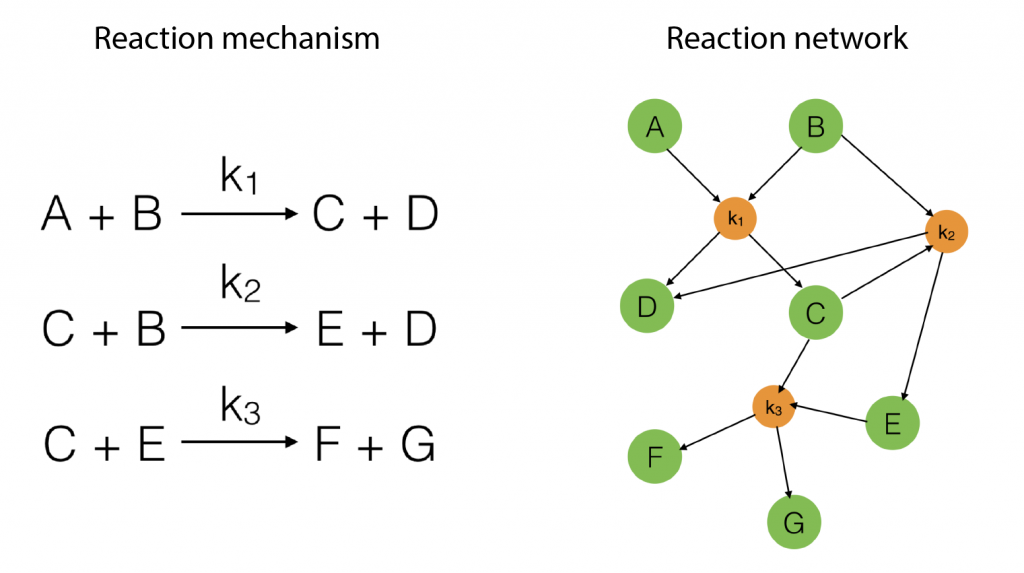
\includegraphics[scale=0.2]{figs/Graph_example.png}
\caption[Graph example to represent Chemical Reactions]{Graph structures in representing chemical reactions mechanisms}
%Source:
\label{fig:Graph_Example}
\end{figure}


\begin{table}
\small
\begin{center}
\begin{tabular}{|c|c|c|c|c|}
\hline
{Network}  &  {Nodes} & {Node features}  & {Edges}  & {Edge features}  \\
\hline
{Transportation System}  &  {cities} & {registered cars}  & {Routes}  & {Length, cost }  \\
\hline
{Banking Network}  &  {Account holders} & {account status}  & {Transactions}  & {Transaction value}  \\
\hline
{Social Network}  &  {users} & {name, country}  & {Interactions}  & {type (like, comment)}  \\
\hline
\end{tabular}
\end{center}
\caption{Some real world graphs}
\label{table:Graph_examples}
\end{table}

\section{Graph classification problem}
\label{sec:Graph_classification_problem}
Graph classification can be understood in several ways. Here, we place ourselves in the context of \emph{supervised learning}, where we suppose we have access to a set of pre-labeled graphs  $(\mathcal{X}=\{\mathcal{G}_1,\ldots,\mathcal{G}_n\}, \mathcal{Y}=\{y_1,\ldots,y_n\})$, where each graph $\mathcal{G}_i$ is \emph{a priori} known to belong to the class with label $y_i$. Stated simply, the graph classification problem we are interested in in this work may be stated as: given this prior information, design a classification algorithm that, given in input any graph (importantly, any graph belonging or not to $\mathcal{X}$), outputs the label of the class to which it belongs. 

More formally, consider the set $\mathcal{D}$ of all graphs $\mathcal{G}$ that can occur in some real-world application, a fixed set of classes $\beta=\{\beta _1,\ldots,\beta _l\}$ of finite size $l$, and a mapping function $f:\mathcal{D}\mapsto\beta$ which maps each graph $\mathcal{G}$ in $\mathcal{D}$ to the class $\beta_\mathcal{G}$ it belongs to. Graph classification is the problem of estimating the mapping function $f$ in the case where it is only known on a subset $\mathcal{X}\subset \mathcal{D}$. Formally, we have a dataset $(\mathcal{X}=\{\mathcal{G}_1,\ldots,\mathcal{G}_n\}, \mathcal{Y}=\{y_1,\ldots,y_n\})$ of size $n$ such that $\mathcal{X}\in \mathcal{D}^n$ and $\mathcal{Y}\in\beta^n$, where for each graph $\mathcal{G}_i\in \mathcal{X}$ we have that $y_i=f(\mathcal{G}_i)$ is the class of $\mathcal{G}_i$. The classification task is to have a \textbf{predictive model} which can predict well, based on some-predefined metric,  the class for any new graph $\mathcal{G}$ in $\mathcal{D}$. This prediction functionality of the model is gained using the dataset $(\mathcal{X}, \mathcal{Y})$ to optimize the parameters of the model that is believed to govern the behavior of the mapping function $f$ on $\mathcal{D}$. This optimization completed in this paradigm is called the learning algorithm.

Note that graph classification as considered here, has nothing to do with the more common problem of \emph{node classification} in a graph, in which there exists only one graph and the goal is to separate the node set in a partition of communities. In our work, graphs are classified, not nodes. This being said, the extra information that the nodes and/or edges may have in some applications (gender, age for instance for nodes of a social network; maximum bandwidth, number of channels for instance for edges of a communication network; etc.) could in principle be used along with the graph structure to classify different graphs into different classes. However, as the existence of such extra-information is very application-dependent, we prefer to focus here on the case where nodes and edges do not carry such information: the only information one has access to for classification is the graph structure.

This problem has been addressed in many different fields of research, such as:
\begin{itemize}
    \item \textbf{\emph{Marketing analytics:}} advertisers and marketers  are interested in detecting the influential people communities in Social Networks in the sense that addressing their products' advertisements to such groups would be a more rewarding investment. This can be approached with graph classification applied on these networks \citep{marketing_analytics}.
    \item \textbf{\emph{Banking security:}} graph classification is used to catch unusual patterns of fraudulent transactions \citep{banking_security}.
    \item \textbf{\emph{Biology and genomics:}} graphs are based on proteins such that nodes correspond
to amino acids which compound the protein and a pair of amino acids are linked by an edge if they are less than 6 Angstroms apart. The task is to detect whether a protein is an enzyme or not \citep{protein_application}, to mention a few.
\end{itemize}

\section{State-of-the-art methods for graph classification}
We  present here existing algorithms for the graph classification problem and discuss their limitations. In general, these algorithms can be classified in four main categories: set based, frequent sub-graph based, kernel based, and graph neural networks based algorithms.\\

\noindent\textbf{Set based algorithms.} This type of algorithms is only applicable to cases where nodes/edges are supplied with features or attributes, as they completely disregard the graph's structure. Based on the provided feature vectors, a distance function of interest between the graphs is computed. % in order to provide a similarity between pairs of edges/nodes in the corresponding sets. 
The drawback of this method is that it does not take the structure (topology) of the graph itself into consideration. For example, if we just compare how much the edges' features of one graph are similar to the edges' features of another, we can have two graphs with the same set of edge features, which will lead to maximum similarity, even though their graph structures can be arbitrarily different. %but we in reality ignore other important information that can make these graphs completely different. % such as how many connected communities of nodes these edges form in each graph, how many circles of nodes these edges promote in each graph, etc. 
On the other hand, a strength of these algorithms is their low computations cost that is usually linear or quadratic in the number of nodes and edges \citep{graphlet_kernel}.\\
 
\noindent\textbf{Frequent sub-graph based algorithms.} These algorithms contain two steps. First, the graph dataset $\mathcal{X}$ is analyzed to enumerate the frequent sub-graphs occuring in the different graphs. Then, another analysis is done to choose the most discriminative sub-graphs out of the ones found during the first step. The disadvantage of using this method is the computational cost that grows exponentially with the graph size \citep{graphlet_kernel}. \\

\noindent\textbf{Graph kernels based algorithms.} It is a middle ground between both previous methodologies, where the graph structure is well considered, and in most cases, these algorithms are designed in a way that the computational time is a polynomial function of the graph size \citep{graphlet_kernel}. However, some effective and competitive kernels still require exponential time, and this is in short the problem we approach in this work using random features to approximate these kernels or to compete with them in notably lower computational time. \\

\noindent\textbf{Graph neural networks (GNNs) based algorithms.} GNNs compute a representation vector (embedding vector) for every node in a graph, where this vector is recursively computed by aggregating the representation vectors of neighboring nodes. The goal of this aggregation technique is that nodes that are neighbors (or close) to each other in the graph are more likely to have similar representations (with respect to some similarity function) and vice versa. On the graph level, a representation vector is computed by aggregating its nodes' representation vectors. This aggregated vector now representing the graph itself is used as a usual feature vector which can be fed to a typical deep neural network to learn the classification task. Traditional GNNs such as graph convolutional networks (GCNs) and GraphSAGE fail to provide high performance classifying graphs whose node/edges don't include any original feature vectors, and that even applies on graphs with simple topology \citep{GCN_powerful}. \nt{I could not re-write this last sentence: I don't understand it} 
However, another GNN structure was developed to overcome this weakness point \nt{complete failure is more than a ``weakness''}, and it is referred to by Graph Isomorphism Network (GIN). Regarding the computational time, it is mainly a matter of the layers number in the network, since this parameter in reality represents how far from a node we want to go in order to compute its representation vector. 

\section{Context and our contribution}
One of the methods of the kernel-based algorithms (the third out of the four categories listed), called graphlet kernel, has proven to be competitive for graph classification. Theoretically and empirically, it was shown that a desired performance or a required amount of information to be preserved from the original graph can be reached with sufficiently large $k$. \nt{**hold your horses! we need at least a few sentences actually \emph{explaining} what is the graphlet kernel you are talking about. For instance, we have yet no clue what $k$ is.**}
However,  the computational cost  becomes prohibitive as $k$ (the graphlet size) and/or $v$ (the size of the graph)  become too large. Thus it cannot be applied on large-scale graph datasets. 

The advent of Optical Processing Units (OPUs) opened a new horizon solving this problem, since it can apply enormous number of \emph{Random Projections} in light speed. \nt{**hold your horses! The reader has no clue \emph{why} making random projections in light speed is actually useful for your problem. You need at least one sentence explaining what you mean by random projections}

In this work, we did the sufficient mathematical analysis to prove that OPUs' light-speed random feature projections compete the $k$-graphlet kernel with respect to \emph{Maximum Mean Discrepancy (MMD)} Euclidean metric. Moreover, we empirically tested this hypothesis and made sure that the the theoretical MMD error is aligned with the empirical one with respect to the parameters introduced in the problem (sampling technique, number of sampled sub-graphs, number of random features, etc). \nt{Instead of this last paragraph, I invite you to write ``Our contributions are the following:'' followed by an ``enumerate'' environment to make a clear and thorough list of your achievements. After that enumeration, I invite you to write ``On top of these contributions, we have also:'' followed by an ``enumerate'' environment to make a list of things you did that we cannot call ``contributions'' yet as they either did not work or are work in progress.}






%\addchapheadtotoc
\chapter{Theoretical Analysis}
We recall that the majority of our work (especially the practical side) focus on using Random Features, mainly OPUs' light-speed random features, to approximate the graphlet kernel to approach Graph Classification problems. We also focus in some stage of this work on using Fourier Random Features to approximate the Gaussian kernel. Thus, in this chapter we first introduce the mathematical notions of Graph Kernels and Random Features. Then, we prove the efficiency of replacing the classical Graph Kernels which have two drawbacks (time, memory) by the use of their corresponding Random Features mapping function, this is to be done using concentration inequalities and information preservation concept. Finally, we show the structure of the OPU and its mathematical model. 

\section{Necessary Notations}
Before proceeding to the analysis of used methods, we first introduce the necessary notations related to Graph definition and Graph kernels.
A graph by definition is a pair $G=(V,E)$, where V is the set of the graph nodes (vertices) $V={v_1,...,v_n}$, and $E\in V\times V$ is the set of edges between these nodes, i.e. $(v_i, v_j)\in E$ means that the graph has an edge from node $v_i$ to node $v_j$ (or vice versa since we consider undirected graphs in this work).
\newline $H=(V_H,E_H)$ is said to be a subgraph (graphlet) of G ($H\sqsubseteq G$) if and only if there exist an injective function $\mathcal{M}:V_H\xrightarrow{} V$ such that $(v,w)\in E_H \Leftrightarrow{(\mathcal{M}(v),\mathcal{M}(w))\in E}$.\newline
Any edge $(v_i, v_i)$ is called a self loop. In a general graph two vertices $v_i$ and $v_j$ may be connected by more than
one edge. A simple graph is a graph with no self loops
or multiple edges. Here we always consider simple graphs.\newline
A simple graph can equivalently be represented by an adjacency matrix $A$ of size $n \times n$. The $(i,j)-th$ entry of $A$ is 1 if an edge $(v_i, v_j)$ exists and zero otherwise.\newline
Two graphs $G=(V,E)$ and $G'=(V',E')$ are isomorphic $(G'\cong G)$ if there exists a bijective function $\mathcal{M}:V\xrightarrow{} V'$ such that $(v_i,v_j)\in E$ iff $(\mathcal{M}(v_i),\mathcal{M}(v_j))\in E'$


\section{Graph Kernels}
The kernel trick is a way to generate features for algorithms that depend only on the inner product between pairs of input points. The mathematical basis behind it is that any positive definite function $k(x,y)$ with $x,y \in \mathcal{R}^d$ defines an inner product and a lifting function $\phi$ so that the inner product between lifted data points equals its kernel $<\phi(x),\phi(y)>=k(x,y)$. The convenience one gets deploying kernels-baed models is that there is no need to access the lifting function $\phi$, instead, the used algorithm accesses the data only through evaluations of $k(x,y)$. To better illustrate this benefit, we take the Gaussian Radial Basis function (RBF) kernel as an example, where:
\begin{equation}
    K_{RBF}(x,y)=exp(-\frac{\left \| x-y\right\|^2}{2\sigma^2})
\end{equation}
where $\sigma$ is called the bandwidth parameter of the kernel. The Hilbert space associated with the Gaussian RBF kernel has infinite dimension, but the kernel may be easily evaluated for any pair (x,y). 

\subsection{Graph kernels design}
Traditional kernel machines approach problems with vector-valued input data, where it compare different objects $(x,y \in \mathcal{R}^d)$ using the difference between vector components. Based on that, these kernels are imperfect to be used with graphs, since the structure of a graph is invariant to permutations of its representation (e.g. Adjacency matrix), i.e. the ordering by which nodes and edges are enumerated, which leads to isomorphic graphs, does not change the graph structure. So in this case distance-kernels between graph representation vectors are uninformative.As a result it is necessary to measure distance between graphs in ways that are themselves permutation invariant. While the concept of isomorphism is important in learning algorithms on graphs,  not only there is no known polynomial-time algorithm for testing graph isomorphism (except for graphs with specific structures), but isomorphism is also too strict for learning in a similar way to learning with equality operator \citep{kriege_graph_kernels}. \newline
The majority of kernels developed to solve graph learning problems are convolution kernels, where given two discrete structures (e.g., two graphs), the idea of convolution framework is to subdivide these to structures into sub-structures (nodes or subgraphs) and evaluate a kernel between each pair of such sub-structures. 
\newtheorem{definition}{Definition} 
\begin{definition}[Convolution Kernel]
let $\mathcal{R}=\mathcal{R}_1\times...\times \mathcal{R}_d$ denote a space of components such that a composite object $X\in \mathcal{X}$ decomposes into elements of $\mathcal{R}$. Let $R:\mathcal{R}\xrightarrow{}\mathcal{X}$ denote the mapping from components to objects, such that $R(x)=X$ iff the components $x\in \mathcal{R}$ make up the object $X\in \mathcal{X}$, and let $R^{-1}(X)=\{x\in\mathcal{R}:R(x)=X\}$. then, the R-convolution kernel is:
\begin{equation}
\label{eq:conolutional_kernels}
    K_{CV}(X,Y)=\sum_{x\in R^{-1}(X)}~\sum_{y\in R^{-1}(Y)}~\underbrace{\prod_{i=1}^{d}k_i(x_i,y_i)}_{k(x,y)}
\end{equation}
with $k_i$ is a kernel on $\mathcal{R}$ for $i\in\{1,...,d\}$.
\end{definition}

Projecting this definition on Graphs, the inverse map $R^{-1}(G)$ of the convolution kernel can be seen as the
set of all components of a graph G that we want to compare. An example of these kernels is the node label kernel whose mapping R takes the attributes $x_u\in \mathcal{R}$ of each node $u\in G\times H$ and maps them to the graph that u is a member of. The attractive advantage using convolution
kernel framework when working with graphs is that while the kernels on substructures are invariant to orderings of nodes and edges, so is the resulting graph kernel. On the other hand, the sum in Eq.~\ref{eq:conolutional_kernels} iterate over all pairs of components. When the considered components become more and more specific, each object becomes increasingly similar to itself, but no longer
to any other objects, this problem is called the diagonal dominance problem, since the entries on the main diagonal of the kernel matrix (Gram matrix) are much higher than other entries,Thus, weights between the components usually are added to balance Gram matrix entries so this drawback is resolved.


\subsection{Graphlet Kernel}
Referring by $\mathcal{G}=\{graphlet(1),..., graphlet(N_k)\}$ to the set of k-nodes graphlets, and considering a graph G of size n we can define a vector $f_G$ of length $N_k$ whose i-th component equals the normalized-number of occurrences of $graphlet(i)$ in G ($\#(graphlet(i)\sqsubseteq G)$. What should be noticed based on this definition is that no two different graphlets in $\mathcal{G}$ are isomorphic. $f_G$ is referred to by k-spectrum of G, and this vector is the key idea behind graphlet kernel. 


\begin{definition}[Graphlet Kernel]
Given two graphs $G$ and $G'$ of size $n,n'\geq k$, the graphlet kernel $k_g$ is defined as \citep{graphlet_kernel}:
\begin{equation}
    k_g(G,G')=f_G^Tf_G'.
\end{equation}
\end{definition}


The drawback of this kernel is that computing the k-spectrum vector costs a lot of computational time, since there are $\tbinom{n}{k}$ size-k subgraphs in a graph G of size n ($O(n^k) $ processing steps required), thus there is a trade off between a more accurate representation of the graph (large value of k) and the computational cost. However, some techniques are used in order to resolve this limitation as Sampling From Graph technique (section \ref{graph_sampling}).

\subsection{Graph Sampling to approximate k-Graphlet Spectrum}
\label{graph_sampling}
The problem of Graph Sampling arises when we deal with a large-scale graph and the task is to pick a small-size sample subgraph/s that would be similar to the original graph with respect to some important properties.\newline
Sampling from graph techniques are used to resolve the processing cost limitation of graphlet kernel, and it can deployed in two different manners:
\begin{enumerate} \itemsep0pt \parskip0pt \parsep0pt
    \item directly sample $m$ sugraphs $\{H_1,...,H_m\}$ of size k, and then estimate the k-spectrum vector empirically:
    $f_G(i)=\frac{1}{m}\Sigma_{j=1}^m \mathbbm{1}[H_j=graphlet(i)]$
    \item sample m subgraphs  $\{H_1,...,H_m\}$ of size $n'$ such that $n\gg n'>k$, then estimate $f_G$ as follows:
    $f_G=\frac{1}{m}\Sigma_{j=1}^m f_{H_j}$, this method is usually being referred to by Mean Kernel Method and is used in problems with large-scale or random distribution-based infinity-size graphs (see \ref{subsec:MMD}).
\end{enumerate}  
The important thing here is whether a sufficiently large number of random samples will lead to an empirical k-spectrum vector close to the actual vector. The number of samples needed to achieve a given confidence with a small probability of error is called the sample complexity. 
\newtheorem{theorem}{Theorem} 
\begin{theorem}
Let $f$ be a probability distribution on the
finite set $\mathcal{G}={g_1,...,g_a}$, $X={X_j}_{j=1}^m$ be a set of independent identically distributed (iid) random variables $X_j$ drawn from $f$, and $\hat{f}(g_i)=\frac{1}{m}\Sigma_{j=1}^m\mathbbm{1}(X_j=g_i)$. Then for a given $\epsilon>0$ and $\delta >0$ we have \citep{graphlet_kernel}:
\begin{equation}
m=\left \lceil \frac{2(log(2)a+log(\frac{1}{\delta} ))}{\epsilon^2} \right \rceil
\end{equation}
samples suffice to ensure that $P\{\left\| f-\hat{f} \right\|_1 \geq \epsilon \}\leq\delta$
\end{theorem}
Therefore this theorem gives a lower bound on the number of samples considered respecting the first manner using Graph Sampling to approximate the k-Graphlet spectrum vector in order to ensure some certainty $\epsilon$ with prabability $(1-\delta)$.
\section{Random Features}
Kernel machines are of interest as they approximate any function arbitrarily well with sufficiently large training data set. On the other hand, the methods that operate on the kernel matrix (Gram matrix) require a lot of time in order to compute this matrix and to train the machine; for example, a dataset with half a million training examples might take days to train on modern workstations \citep{rahimi2008random}.
Unlike kernel machines, linear support vector machines and regularized regression run much faster especially with low-dimensionality training data. 
One way to combine the advantages of the linear and nonlinear vector machines is to convert the training and evaluation of any kernel machine into the corresponding operations of a linear machine by mapping data into a relatively low-dimensional randomized feature space.
Instead of considering the implicit lifting function which corresponds to the kernel, it was proposed to explicitly map the data to a low-dimensional Euclidean inner product space using a randomized feature map $z:\mathcal{R}^d \xrightarrow{}\mathcal{R}^D$ so that the inner product between a pair of transformed points approximates their kernel:
\begin{equation}
\label{eq:approx_RF}
k(x,y)=<\phi(x),\phi(y)> \approx z(x)^Tz(y)
\end{equation}
Considering this approximation, we can simply transform the input with $z$ and then apply a fast linear learning method to approximate the answer of the real kernel. \newline
In what follows, Random Fourier Features method to construct the random feature map function $z$ is presented.

\subsection{Random Fourier Features}
The following Theorem represents the key idea behind this mapping technique
%\newtheorem{theorem}{Theorem}
\begin{theorem}[Bochner's theorem]
A continuous and shift-invariant kernel $k(x,y)=k(x-y$ on $\mathcal{R}^d$ is positive definite if and only if $k(\delta)$ is the Fourier transform of a non-negative measure.
\end{theorem}
What that means is that when a shift-invariant kernel $k$ is properly scaled, its Fourier transform $p(w)$ is a proper probability distribution, we can write:
\begin{equation}
\label{Fourier integral}
k(x-y)=\int_{\mathcal{R}^d}p(w)e^{j{w}'(x-y)}dw=E_w[e^{j{w}'x}{e^{j{w}'y}}^*]
\end{equation}
But both $p(w)$ and $k(\delta)$ are real-valued functions, thus from Eq.~\ref{Fourier integral} we can prove that:
\begin{equation}
\label{real Fourier integral}
k(x-y)=\int_{\mathcal{R}^d}p(w)cos({{w}'(x-y)})dw=E_w[z_w(x)z_w(y)]
\end{equation}
where $z_w(x)=\sqrt{2}cos({w}'x+b)$ such that $w$ is drawn from $p(w)$ and b is drawn uniformly from $[0,2\pi]$.\newline
As a straight result, $\ z_w(x)z_w(y)$ is an unbiased estimate of k(x,y). We can achieve lower variance estimation to the expectation (Eq. \ref{real Fourier integral}) by averaging $D$ instances of the estimator with different random frequencies $w$. i.e. the low-variance estimator can be written as: $z(x)'z(y)=\frac{1}{D} \Sigma_{j=1}^D z_{w_j}(x)z_{w_j}(y)$. this estimator and based on Hoeffding's inequality guarantees exponentially fast convergence in $D$ between $z(x)'z(y)$ and the kernel true value:
\begin{equation}
    Pr(|z(x)'z(y)-k(x,y)|\geq\epsilon)\leq2e^\frac{-D\epsilon^2}{4}
\end{equation}

\subsection{Random features from compressed sensing's  point of view}
Random features can be tackled within a different paradigm in signal processing, in compressed sensing for instance a random projection of a high-dimensional but sparse or compressible signal onto a lower-dimensional space has been shown to contain enough information to be used to reconstruct the original signal with small error margins. In this domain, the well-known Johnson-Lindernstrauss (JL) lemma states that with high probability the geometry of a point cloud is preserved by certain Lipschitz mapping onto a space of dimension logarithmic in the number of points, and with the help of concentration inequalities for random inner products more efficient algorithms for constructing such embeddings were developed. First, we recall $\ell_p^N$ norm of a vector $x\in\mathcal{R}^N$:
\begin{equation}
    \left \| x\right\|_{\ell_p^N}=
    \left\{\begin{matrix}
{(\Sigma_{i=1}^N x_i^p)}^\frac{1}{p}\qquad,  0<p<\infty\\ 
max_{i=1,...,N}\left \| x_i\right\|~~\quad, p=\infty
\end{matrix}\right.
\end{equation}
In the discrete compressed sensing, we want to economically record information about a vector $x\in \mathcal{R}^N$, thus we allocate a group of n nonadaptive questions to ask about $x$. Each question takes the form of a linear function applied to $x$, i.e. the extracted information can be written in the form: 
\begin{equation}
    y=\phi x
\end{equation}
where $\phi \in \mathcal{R}^{n\times N}$ and $n$ is much smaller than $N$. \newline
To reconstruct the original signal from the information that $y$ holds about $x$, a decoder $\Delta$ is used to provide an approximation $\bar{x}=\Delta(y)=\Delta(\phi x)$. It should be noticed in our case with graph classification problem using random features that it is not one of our concerns to find or prove the proficiency of any decoder, but it is important to cover the mathematics that prove the efficiency of random projections represented in compressed sensing by the pair $(\phi, \Delta)$ . to measure the performance of an encoder-decoder pair $(\phi, \Delta)$, we use a norm $\left\| .\right\|_X$ to quantify the error: 
\begin{equation}
    e(x,\phi,\Delta)_X=\left\| x-\Delta(\phi x)\right\|_X
\end{equation}
which is the error of the pair $(\phi, \Delta)$ on $x$. Moreover, if K is any compact set in $\mathcal{R}^N$, then the error of this pair on K is:
\begin{equation}
    e(K,\phi,\Delta)_X = \underset{x\in K}{sup} ~e(x,\phi,\Delta)_X
\end{equation}
To find the best pair that minimizes the previous error, we introduce the set $\mathcal{A}_{n,N}=\{(\phi, \Delta ): \phi \in \mathcal{R}^{n\times N}\}$, thus the best performance of such pair on $K$ is given by: 
\begin{equation}
e_{n,N}(K)_X= \underset{(\phi, \Delta)\in \mathcal{A}_{n,N}}{inf}~e(K,\phi,\Delta)_X
\end{equation}
However, it was proven that if $K\subset \mathcal{R}^N$ such that $K=-K$ and that $K+K\subset C_1K$ ,where $C_1$ is a constant, then\citep{concentration_kashin}:
\begin{equation}
\label{3.5}
   d^n(K)_X < e_{n,N}(K)_X<C_1d^n(K)_X
\end{equation}
where $d^n(K)_X$ is Gelfand width of $K$ in the Banach space $X$:
\begin{equation}
    d^n(K)_X= \underset{codim(Y)=n}{inf}~\underset{x\in K\cap Y}{sup}\left\|x\right\|_X
\end{equation}
Here the best spaces $Y$ are those that slice through $K$ in the most economical direction to minimize the diameter of the set $K\cap Y$ (which corresponds to the direction with minimum variance notion used in Principle Component Analysis PCA). An important result of Gelfand widths that can be used in our paradigm is the limits of this width on the unit ball $K=U(\ell_1^N)$, it states that there exists a constant $C_0>0$ such that the following condition is satisfied whenever $0< n< N $:
\begin{equation}
    C_0^{-1}\sqrt{\frac{log(N/n)+1}{n}}\leq d^n(U(\ell_1^N))_{\ell_2^N}\leq C_0\sqrt{\frac{log(N/n)+1}{n}}
\end{equation}
Back to the proof of Eq.~\ref{3.5} Which can be done by checking the correspondence between $Y$ and $\phi$, where given any matrix $\phi$, its null space $\mathcal{N}$ is a valid candidate for $Y$ in computing $d^n(K)_X$. On the other hand, given any $Y$ of co-dimension $n$ used in computing $d^n(K)_X$, any basis for the orthogonal complement of $Y$ can be used as the rows of a matrix $\phi$ to estimate $E_{n,N}(K)_X$. For example, the unit ball $U(\ell_1^N)$ in $\ell_2^N$ satisfies that $U(\ell_1^N)+U(\ell_1^N)\subset 2U(\ell_1^N)$, thus for all $0< n< N$ : 
\begin{equation}
\label{3.6}
    C_0^{-1}\sqrt{\frac{log(N/n)+1}{n}}\leq E_{n,N}(U(\ell_1^N))_{\ell_2^N}\leq 2C_0\sqrt{\frac{log(N/n)+1}{n}}
\end{equation}
The main problem then is to find the pair $(\phi, \Delta)$ which provides estimates like Eq.~ \ref{3.6}, to address this question an isometry condition on $\phi$ was introduced. Given a matrix $\phi$ and any set T of column indices, we refer by $\phi_T$ to the $n\times \#(T)$ matrix composed of these columns. Simultaneously, for every $x\in \mathcal{R}^N$, we refer by $x_T$ to the vector obtained by considering only the entries in $x$ which correspond to the column indices $T$. We say that a matrix $\phi$ satisfies the RIP (Ristricted Isometry Property) of order k if there exists a $\delta_k\in [0,1]$ such that:
\begin{equation}
    \label{3.8}
    (1-\delta_k)\left\|x_T\right\|_{\ell_2^N}^2\leq
    \left\|\phi_Tx_T\right\|_{\ell_2^N}^2\leq  (1+\delta_k)\left\|x_T\right\|_{\ell_2^N}^2
\end{equation}
holds for every such set $T$ with $\#T\leq k$. The good matrices $\phi$ should satisfy the RIP condition for the largest possible $k$. For instance, if $\phi$ satisfies the RIP of order $3k$ with $\delta_{3k}<1$, then:
\begin{equation}
\label{3.9}
\left\|x-\Delta(\phi x)\right\|\leq \frac{c_2\sigma_k(x)_{\ell_1^N}}{\sqrt(k)}
\end{equation}
where $\sigma_k(x)_{\ell_1^N}$ is the $\ell_1$ error of the best k-term approximation and the constant $C_2$ depends only on $\delta_{3k}$. Since $\sigma_k(x)_{\ell_1^N}\leq \left\|x\right\|_{\ell_1^N}$ , we can obtain the best possible performance correspondent to Eq.\ref{3.6} if we can find a matrix $\phi$ that meet the RIP condition for $k$ of order $n/(log(N/n)+1)$.\newline
Now the question is how to construct such matrix $\phi$ that satisfy the RIP for the largest possible range of $k$. Actually, the only known constructions yielding such matrices are based on random matrices \citep{concentration_kashin}. It is shown that matrices built using random entries drawn from certain probability distributions will meet the RIP Condition with high probability. More specifically, for these constructions of $\phi$, the RIP follows in a simple way from the same concentration of measure inequalities for inner products that have employed to prove the JL lemma (which will not be stated here being irrelevant). \newline
Briefly, it is shown \citep{concentration_achlioptas} that any random variable which satisfies certain moment conditions, the matrix $\phi$ whose entries are independent realizations of this variable can be proven to satisfy the following concentration inequality for any $\epsilon \in [0,1]$:
\begin{equation}
\label{4.3}
    Pr(|~ \left\| \phi x\right\|_{\ell_2^N}^2- \left\|x \right\|_{\ell_2^N}^2~|\geq \epsilon\left\| x\right\|_{\ell_2^N}^2 )\leq 2e^{-nc_0(\epsilon)}
\end{equation}
Where $c_0(\epsilon)$ is only a function of $\epsilon$. The point now is to prove satisfying Eq.\ref{4.3} with some covering arguments is sufficient to prove the RIP for the corresponding matrix $\phi$, then some examples of these distributions are presented.
Considering the same aforementioned notation $\phi_T, X_T$ with $\#T\leq k$ with $\ell_2$ norm, the proof includes constructing  nets of points in each k-dimensional subspace, apply \ref{4.3} to all of these points through a union bound, and then extend the result from our finite set of points to all possible k-dimensional signals. 
\newtheorem{lemma}{Lemma} 
\begin{lemma}
let $\phi(w), w\in \omega^{n\times N}$, be  a random matrix of size $n\times N$ drawn from any distribution that satisfies the concentration inequality (\ref{4.3}). Then, for any set T with $\#T= k<n$ and any $0< \delta< 1$, we have
\begin{equation}
(1-\delta) \| x\|_{\ell_2^N}  
\leq
\| \phi(w)x\|_{\ell_2^N} 
\leq
(1_+\delta) \| x\|_{\ell_2^N} ~for ~all ~x\in X_T
\label{5.1}
\end{equation}
with probability
\begin{equation}
\geq 1-2(12/\delta)^k e^{-c_0(\delta/2)n}
\label{5.2}
\end{equation}

\end{lemma}

The first step of the proof is noticing that since $\phi$ represents a linear transformation, it is enough to prove \ref{5.1} in the case $\|x\|_{\ell_2^N}=1$. The next step is to choose a finite set of points $Q_T\subset X_T$ with $\|q\|_{\ell_2^N}=1$ for all $q\in Q_T$, that satisfies:
\begin{equation}
    \underset{q\in Q_T}{min}~ \|x-q\|_{\ell_2^N}\leq\delta/4 ~~for ~all ~x\in X_T
\end{equation}
The existence of such group is proven within the scope of covering numbers where also we can find that $\#Q_T\leq (12/\delta)^k$. Now, using the union bound to apply \ref{4.3} to this $Q_T$ with $\epsilon=\delta/2$, with
probability exceeding the right side of \ref{5.2}, we have:
\begin{equation}
(1-\delta/2) \| q\|_{\ell_2^N}  
\leq
\| \phi(w)q\|_{\ell_2^N} 
\leq
(1+\delta/2) \| q\|_{\ell_2^N} ~for ~all ~q\in Q_T
\end{equation}
Let A be the smallest number such that:
\begin{equation}
     \| \phi(w)x\|_{\ell_2^N} \leq (1+A) \| x\|_{\ell_2^N} ~for ~all ~x\in X_T
\label{5.6}
\end{equation}
But there is $q\in Q_T$ such that $\| x-q\|_{\ell_2^N}\leq \delta/4 $, so we have:
\begin{equation}
    \| \phi(w)x\|_{\ell_2^N} \leq
    \| \phi(w)q\|_{\ell_2^N} +
    \| \phi(w)(x-q)\|_{\ell_2^N} \leq
    1+\delta/2 +(1+A)\delta/4
    \label{5.7}
\end{equation}
By a simple comparison between Eq.\ref{5.6} and Eq. \ref{5.7}, we get that $A\leq \delta$, which is what we seek proving the upper inequality in Eq. \ref{5.1}, and the lower one can be proven in a similar way.
\begin{theorem}
when n<N, and $0< \delta< 1$,  If the probability distribution generating the $n\times N$ matrices $\phi(w), w\in \Omega^{n\times N}$, satisfies the concentration inequality \ref{4.3}, then there exist constants $c_1, c_2> 0$ depending only on $\delta$ such that
the RIP condition holds for $\phi(w)$ with the prescribed $\delta$ and any $k \leq c_1n/log(N/k)$ with probability $\leq 1-2e^{-c_2n}$.
\end{theorem}
To prove this theorem, from Eq.\ref{5.1} we know that the matrix $\phi(w)$ doesn't satisfy the inequality with probability $\leq 2(12/\delta)^ke^{-c_0(\delta/2)n}$ for each of the k-dimensional sub-spaces. But there are $\binom{N}{k}\leq (eN/k)^k$ such sub-spaces. Thus, this probability for all the sub-spaces becomes: 
\begin{equation}
    \leq  2(eN/k)^k(12/\delta)^ke^{-c_0(\delta/2)n}=2e^{-c_0(\delta/2)n+k[log(12/\delta)+log((eN/k))]}
\label{5.10}
\end{equation}{}
So for a fixed $c_1>0$, and $k\leq c_1n/log(N/k) $, we have that the exponent in Eq. \ref{5.10} is $\leq -c_2n$ provided that $c_2\leq c_0(\delta/2)-c_1[1+(1+log(12/\delta))/log(N/k)]$. Hence, when $c_1>0$ is sufficiently small we have $c_2>0$. So this is what we seek, This proves that with probability $1-2e^{-c_2n}$, the matrix $\phi(w)$ will satisfy Eq. \ref{5.1} on all the k-dimensional sub-spaces for the range of $k\leq c_1' n/[log(N/n) + 1]$ for $c_1'$ depending only on the aforementioned $c_1$.\newline 
The main example of such distributions that satisfy the inequality in \eqref{4.3} (so the moments of it satisfy the prerequisites of this inequality)  is the random matrix $\phi$ whose entries are independent realizations of Gaussian random variable \citep{concentration_kashin}:
\begin{equation}
    \phi_{i,j}\sim \mathcal{N}(0,\frac{1}{n})
\end{equation}
Where the corresponding constant $c_0$ is $c_0(\epsilon)=\epsilon^2/4-\epsilon^3/6$.
Another two examples related to Bernouli distribution which has the same value of the constant $c_0(\epsilon)$:
\begin{equation}
    \phi_{i,j}= 
    \left\{\begin{matrix}
    +1/\sqrt{n} ~ with ~probability ~\frac{1}{2}
\\ 
-1/\sqrt{n} ~ with ~probability ~\frac{1}{2}
\end{matrix}\right.
\end{equation}

\begin{equation}
    \phi_{i,j}= 
    \left\{\begin{matrix}
    +\sqrt{3/n} ~ with ~probability ~\frac{1}{6}
\\ 
0 ~ with ~probability ~\frac{2}{3}
\\
 -\sqrt{3/n} ~ with ~probability ~\frac{1}{6}

\end{matrix}\right.
\end{equation}


\subsection{Mean kernel and random features} \label{subsec:MMD}
%\paragraph{Mean kernel and MMD} 
The mean kernel methodology allows to \emph{lift} a kernel from a domain $\mathcal{X}$ to a kernel on \emph{probability distributions} on $\mathcal{X}$. Given a base kernel $k$ and two probability distribution $P,Q$, it is defined as
\begin{equation}\label{eq:mean_kernel}
k(P,Q) = \mathbb{E}_{x \sim P, y \sim Q} k(x,y)
\end{equation}
In other words, the mean kernel is just the expectation of the base kernel with respect to each term. The associated Euclidean metric is referred to by the  \emph{Maximum Mean Discrepancy (MMD)}, and is naturally defined as:
\begin{equation}\label{eq:MMD}
MMD(P,Q) = \sqrt{k(P,P) + k(Q,Q) - 2k(P,Q)}
\end{equation}
It should be noticed here that $k(P,P) = \mathbb{E}_{x \sim P, x' \sim P} k(x,x') \neq \mathbb{E}_{x \sim P} k(x,x)$.
NOw given data points $(x_1, \ldots, x_n)$ drawn $iid$ from $P$ and $(y_1, \ldots, y_n)$ drawn $iid$ from $Q$, the kernel in Eq. \ref{eq:mean_kernel} can naturally be approximated by:
\begin{equation}\label{eq:mean_kernel_approx}
k(P,Q) \approx \frac{1}{n^2} \sum_{i,j=1}^n k(x_i,y_j)
\end{equation}
and the corresponding approximate MMD is (other variants exist):
\[
MMD(P,Q) \approx \sqrt{\frac{1}{n^2} \sum_{i,j=1}^n k(x_i,x_j) + k(y_i,y_j) - k(x_i,y_j) - k(x_j, y_i)}
\]

\paragraph{MMD and random features}
Mean kernel works especially well with random features. Combining \eqref{eq:approx_RF} and \eqref{eq:mean_kernel_approx}, it is not hard to see that using random features the mean kernel can be further approximated by:
\begin{equation}
\label{eq:mean_kernel_RF}
k(P,Q) \approx \frac{1}{n^2} \sum_{i,j=1}^n \phi(x_i)^*\phi(y_j) = \left(\frac{1}{n} \sum_i \phi(x_i)\right)^* \left(\frac{1}{n} \sum_i \phi(y_i)\right)
\end{equation}
So the computation can be drastically improved by first computing the \emph{averaged random features} (also called random \emph{generalized moments}, also called \emph{sketch}) $\frac{1}{n} \sum_i \phi(x_i)$, and taking a linear kernel between them. The corresponding MMD is then just the Euclidean metric between the averaged random features
\[
MMD(P,Q) \approx \| \frac{1}{n} \sum_i \phi(x_i) - \frac{1}{n} \sum_i \phi(y_i)\|_2
\]

\paragraph{MMD for discrete distributions}
for a discrete space of objects $H_1, \ldots, H_N$ with discrete probability distributions $P = [P_1, \ldots, P_N]$ and $Q$ on them, the mean kernel \ref{eq:mean_kernel} takes a particular form:
\[
k(P,Q) = \sum_{i,j=1}^N P_i Q_j k(H_i, H_j)
\]

\paragraph{MMD with random features on discrete distrbutions}

To combine both notions One can see the link with graphlet sampling, where $f_G$ is the (discrete) probability distribution of the graphlets. If we define $k(F, F') \approx \phi(F)^*\phi(F')$ where $\phi$ is a random feature map that replaces $\phi_k$, then the feature map \eqref{eq:graphlet_kernel_approx} is exactly what appears in \eqref{eq:mean_kernel_RF}. So, now, all the game becomes to find a good feature map $\phi(F)$ for graphlets. The induced MMD metric between graphs is the MMD between graphlets probability distributions $f_G$:
\[
d(G,G') = MMD(f_G, f_{G'}) = \sqrt{k(f_G, f_{G}) + k(f_{G'}, f_{G'}) - 2 k(f_G, f_{G'})} \approx \| \frac{1}{n} \sum_i \phi(F_i) - \frac{1}{n} \sum_i \phi(F'_i)\|_2
\]
where $F_i$ are graphlets drawn from $G$ and $F'_i$ are graphlets drawn from $G'$.






\section{Random Projections with Optical Processing Units (OPU's)}
Random projections is one of the important techniques in machine learning and signal processing, but it requires either to store a very large random matrix, or to use a
different, structured matrix to reduce the computational and memory costs. Optical processing units (OPU's) are the tools used to overcome this difficulty, an OPU performs random projections at the speed of light without having to store any matrix in memory. In general, Random projections are the result of two procedures where the first one is the linear-random projections and the second one is non-linear mapping.
Mathematically speaking, OPU's perform the following operation \citep{saade_opu}:
\begin{equation}
\label{OPU_equation}
    X=\phi(WU+b);~W\in \mathcal{R}^{r\times d},b\in \mathcal{R}^r, U\in \mathcal{R}^d
\end{equation}
where $W$ is the random projection matrix, b is a bias, U is an input point, r is the number of random features and d is the input space dimension.With, $W$ is a random i.i.d complex matrix with Gaussian real and imaginary parts and $\phi$ is the non-linear mapping function.\newline
In the limit where the number of random features $r\xrightarrow{}\infty$, it can be proven by the concentration of the measure that the inner product between the projected data points $(X_i\in \mathcal{R}^r)$ in the new feature space tends to a kernel function that depends only on the input points in the original feature space $(U_i\in \mathcal{R}^d)$

\subsection{OPU structure and functionality}
Eq.~\ref{OPU_equation} still imply that an OPU need to store and multiply by the random projection matrix.\newline
In such units a heterogeneous material, such as paper or any white translucid material, is used to scatter incident light in a very complex way, so the behavior of light scattering is considered random because of the extremely high complexity. one can argue that light scattering is a linear, deterministic, and reproducible phenomenon, but what can be said is that the unpredictable nature of the process makes it effectively a random process, that is why these materials are called opaque since all information carried within the incident light is seemingly lost during the propagation through the material \citep{saade_opu}. An example used to demonstrate and justify the resulted randomness is a cube of edge length $100\mu m$, such cube can comprise $\approx 10^7$ paint nanoparticles, all the positions and shape of these particles must be known in order to predict its effect on light. Propagation through such a layer can be seen as a random walk because of frequent scattering with the nanoparticles, where light would explore the whole volume
and endure on average tens of thousands of such scattering steps before exiting on the other side in a few picoseconds.\newline

\begin{figure}[ht!]
\begin{center}
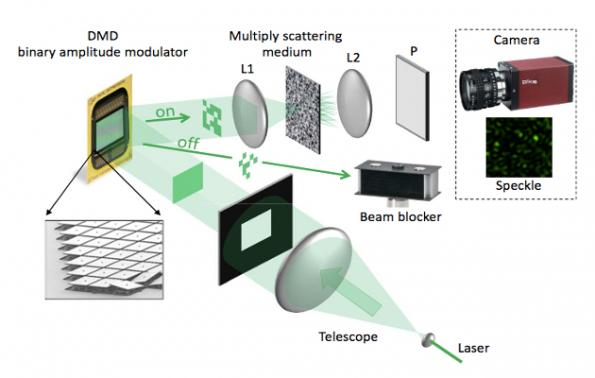
\includegraphics[scale=0.5]{figs/lighton630.jpg}
\end{center}
\caption[OPU's Experimental setup]{OPU's Experimental setup \citep{saade_opu}: A monochromatic laser is expanded by a telescope, then
illuminates a digital micromirror device (DMD), able to spatially encode digital information on the light beam by
amplitude modulation. The light beam carrying the signal is then focused on a random
medium by means of a lens. The transmitted light is collected on the
far side by a second lens, passes through a polarizer, and is measured by a standard monochrome CCD camera for example .}


\label{fig_opu}
\end{figure}


When the incident light is coherent, it gives rise to interferences, and the complex interference pattern arising from the multiple scattering process is called speckle. These patterns are not characteristic only of the propagation medium but also of the shape of the incident light, and this can be modeled by $y=Wx$, where y and x are the vector amplitudes between a set of spatial modes at the output and at the input of the medium respectively and $W$ is the transmission matrix of the medium and it was shown to be very close to Gaussian i.i.d matrices \citep{saade_opu}. What's more convenient to use the aforementioned configuration as a platform for random projections, even without W being determined, is that for a stable medium, such as a paint layer, the transmission matrix $W$ is stable as well. 
So lightening this layer with an appropriate set of incident illuminations, which is possible using a spatial light modulator and a laser, and measuring the output speckle using CCD or CMOS camera, we can record the resulting intensity $|y|^2$, which is the principle concept behind OPU's functionality as seen in Fig~ \ref{fig_opu}.\newline
The DMD (digital micromirror device) used in OPU's is a Binary Amplitude Modulator consisting of an array of micro-mirrors, Each encodes a binary value(lit or not). In order to represent grey values, each value is encoded on a square sub-array ($4\times 4$ for example) in the DMD,where the number of lit mirrors reflects the desired level of grey. DMD reflects the data through the disordered medium, and a snapshot of the resulting random projection is acquired using a standard camera, all that in a very high speed compared to the traditional random features techniques. 



\iffalse
Example of double quotes ``word''. Lorem ipsum dolor sit amet, consectetur adipiscing elit. Curabitur viverra, velit eget vestibulum viverra, nisl eros aliquet sapien, sed interdum tellus justo et purus. Nulla vel orci nisl. Curabitur porta lacinia quam, finibus bibendum mi tincidunt eget. Aenean aliquam lobortis orci, ut aliquam neque imperdiet vel. Nunc sit amet scelerisque velit. Aenean quis tempor leo, at consectetur ipsum. Nam ac urna dapibus, condimentum orci a, ornare ante. In hac habitasse platea dictumst. 
\subsection{Another subsection of section - citations}
Example of citation \citep{altschul1997gapped}. Mauris nisi felis, pharetra vitae velit at, sollicitudin molestie justo. Aenean tristique diam pulvinar, semper risus sed, mattis elit. Phasellus interdum erat at enim maximus interdum. Curabitur tempor, arcu nec malesuada facilisis, tortor nisi ornare ex, ut porttitor elit lectus aliquam diam. Cum sociis natoque penatibus et magnis dis parturient montes, nascetur ridiculus mus. Vivamus quam turpis, auctor in nunc nec, varius pharetra nibh. Ut sagittis diam nec dui sodales tempor. Integer molestie diam id quam placerat eleifend. Nulla posuere iaculis nisi, et sagittis ipsum consequat scelerisque. In nec turpis eget tellus pulvinar porttitor vitae ac tortor. Nullam tempor ut orci ac porttitor. Pellentesque aliquam lacinia gravida. Duis accumsan tristique augue, vitae aliquam magna convallis ac. Aenean vel diam non eros venenatis ullamcorper sit amet at augue. 


Example of multiple citations \citep{altschul1997gapped,baker2007novel}. Nullam mollis et leo at pharetra. Nulla efficitur molestie euismod. Sed dapibus metus sed tempus varius. Aenean finibus eros ut urna luctus feugiat. Duis turpis risus, viverra vitae porta et, ullamcorper ac est. Proin in eros nec ipsum interdum tempus. Nam fringilla lectus velit, non posuere ex vehicula ut. Mauris tincidunt, dolor sit amet commodo tempor, erat mi egestas dui, at elementum tellus est rhoncus libero. Ut et rutrum lectus, id viverra tortor. Vivamus nec lacus eros. Donec dictum porta nisi et vestibulum. Mauris luctus ligula ut libero aliquet luctus. Quisque malesuada egestas finibus. 
\subsubsection{Subsubsection of section - italic text}
Example of italic text - {\it Escherichia}, {\it Salmonella}, and {\it Shigella} spp. Mauris dictum pharetra fermentum. Maecenas ut felis varius, dapibus sapien imperdiet, dictum dui. Proin feugiat viverra metus non laoreet. Integer pulvinar mi id lacus semper commodo. Praesent vel erat interdum purus scelerisque maximus. Sed enim risus, mollis blandit ligula ac, sagittis venenatis augue. Mauris nisi purus, gravida ac aliquam eu, ullamcorper eget nulla. Proin id finibus purus. Vestibulum leo ante, porta in quam sed, eleifend feugiat arcu. Nunc viverra fringilla turpis a iaculis. In condimentum aliquet mauris, quis laoreet eros porta eu. Aenean ut turpis a massa gravida pretium. Phasellus auctor purus quis diam interdum, nec luctus lorem auctor. Pellentesque finibus elit justo, a vulputate diam fermentum lacinia. 
\section{Another section}
Mauris dictum pharetra fermentum. Maecenas ut felis varius, dapibus sapien imperdiet, dictum dui. Proin feugiat viverra metus non laoreet. Integer pulvinar mi id lacus semper commodo. Praesent vel erat interdum purus scelerisque maximus. Sed enim risus, mollis blandit ligula ac, sagittis venenatis augue. Mauris nisi purus, gravida ac aliquam eu, ullamcorper eget nulla. Proin id finibus purus. Vestibulum leo ante, porta in quam sed, eleifend feugiat arcu. Nunc viverra fringilla turpis a iaculis. In condimentum aliquet mauris, quis laoreet eros porta eu. Aenean ut turpis a massa gravida pretium. Phasellus auctor purus quis diam interdum, nec luctus lorem auctor. Pellentesque finibus elit justo, a vulputate diam fermentum lacinia. 
\section{Another section}
Mauris dictum pharetra fermentum. Maecenas ut felis varius, dapibus sapien imperdiet, dictum dui. Proin feugiat viverra metus non laoreet. Integer pulvinar mi id lacus semper commodo. Praesent vel erat interdum purus scelerisque maximus. Sed enim risus, mollis blandit ligula ac, sagittis venenatis augue. Mauris nisi purus, gravida ac aliquam eu, ullamcorper eget nulla. Proin id finibus purus. Vestibulum leo ante, porta in quam sed, eleifend feugiat arcu. Nunc viverra fringilla turpis a iaculis. In condimentum aliquet mauris, quis laoreet eros porta eu. Aenean ut turpis a massa gravida pretium. Phasellus auctor purus quis diam interdum, nec luctus lorem auctor. Pellentesque finibus elit justo, a vulputate diam fermentum lacinia. 

\chapter{LINKS}
\section{Chapter one tittle section - links examples}
Example of hyperlink \url{http://www.wikibooks.org}. Fusce ultricies pulvinar diam sed ultrices. Sed orci justo, rutrum in dolor a, consequat dictum mi. Sed luctus congue ex nec dignissim. Phasellus volutpat urna vestibulum ipsum vestibulum, quis venenatis justo consectetur. Nullam hendrerit nisl in rutrum convallis. Sed sit amet malesuada nisi. Phasellus dolor neque, vehicula vestibulum semper at, facilisis eget libero. Mauris interdum magna molestie, auctor felis a, condimentum odio. Pellentesque habitant morbi tristique senectus et netus et malesuada fames ac turpis egestas. Suspendisse maximus lacinia dignissim. Maecenas pharetra accumsan metus, sagittis dictum purus sollicitudin eget. Curabitur ut porttitor arcu, ut porttitor ipsum. Vestibulum porttitor finibus sapien, ac pharetra odio bibendum nec. Nullam tincidunt dignissim risus imperdiet dictum.

Pellentesque habitant morbi tristique senectus et netus et malesuada fames ac turpis egestas. Suspendisse maximus lacinia dignissim. Maecenas pharetra accumsan metus, sagittis dictum purus sollicitudin eget. Curabitur ut porttitor arcu, ut porttitor ipsum. Vestibulum porttitor finibus sapien, ac pharetra odio bibendum nec. Nullam tincidunt dignissim risus imperdiet dictum.
\subsection{Subsection title - more links examples}.
Another example of hyperlink \href{http://www.wikibooks.org}{Wikibooks home}. Nullam mollis et leo at pharetra. Nulla efficitur molestie euismod. Sed dapibus metus sed tempus varius. Aenean finibus eros ut urna luctus feugiat. Duis turpis risus, viverra vitae porta et, ullamcorper ac est. Proin in eros nec ipsum interdum tempus. Nam fringilla lectus velit, non posuere ex vehicula ut. Mauris tincidunt, dolor sit amet commodo tempor, erat mi egestas dui, at elementum tellus est rhoncus libero. Ut et rutrum lectus, id viverra tortor. Vivamus nec lacus eros. Donec dictum porta nisi et vestibulum. Mauris luctus ligula ut libero aliquet luctus. Quisque malesuada egestas finibus.
 
\section{Another Section}
\subsection{Subsection title}.
Pellentesque habitant morbi tristique senectus et netus et malesuada fames ac turpis egestas. Suspendisse maximus lacinia dignissim. Maecenas pharetra accumsan metus, sagittis dictum purus sollicitudin eget. Curabitur ut porttitor arcu, ut porttitor ipsum. Vestibulum porttitor finibus sapien, ac pharetra odio bibendum nec. Nullam tincidunt dignissim risus imperdiet dictum.
\fi
\newcommand{\todoNK}[1]{\textbf{\textcolor{red}{NK: #1}}}
\chapter{Background}
\label{chapter:background}
\newtheorem{theorem}{Theorem}
In this chapter we present the necessary background that the reader should have in order to proceed through the next two chapters, which are the core of this work. After a brief overview of kernel methods in machine learning, we will present random features and graph kernels. In the next chapter, these different notions will be combined in the proposed algorithm.

\section{Kernel methods and random features}

We first start by an overview of kernel methods.

\subsection{Kernel methods and kernel trick}
Kernel methods is a family of classic algorithms in machine learning that learn models as a combination of similarity functions between data points $(x,x')$, defined by positive semi-definite (psd) \emph{kernels} $\mathcal{K}(x,x')$. Denote by $\mathcal{D}$ the set of all possible data points. A symmetric function $\mathcal{K}:\mathcal{D}\times\mathcal{D}\mapsto\mathbb{R}$ is said to be a positive semi-definite kernel if:
\begin{equation}
\forall n\in \mathbb{N},~\forall \alpha_1,\ldots,\alpha_n\in \mathbb{R},~\forall x_1,\ldots,x_n\in \mathcal{D},\quad \sum_{i,j}^n\alpha_i\alpha_j\mathcal{K}(x_i,x_j)\geq 0 \, .
\end{equation}
\nt{Can we \emph{not} use mathcal for a function? I suggest $\kappa$}

Let us now illustrate how kernels can be incorporated to learning models and how that is useful to learn more complex functions. To do that let us consider a simple classification problem: take $\mathcal{D}=\mathbb{R}^d; d\in\mathbb{N}$, and let $(\mathbf{X},\mathbf{Y})$ be a labeled dataset of size $n$ with datapoints $\mathbf{X}\in \mathbb{R}^{n\times d} $ and labels $\mathbf{Y}\in \{-1,1\}^n$. \nt{and here $X$ and $Y$ should be mathcal right? Ok, I'll stop here for notation comments as I recall you were saying that you had not changed notations yet. Also I guess you'll need to define the vector $\mathbf{y}$ where $y_i$ is the label of $\mathbf{x}_i$} Many of the learning models designed to solve this problem, like Support Vector Machine (SVM) \nt{add ref} and Perceptron binary classifier \nt{add ref}, rely on the inner product as a measure of similarity between data points: during the training, they only use inner products $\mathbf{x}_i^T \mathbf{x}_j$, and then produce models with the following form \citep{inner_product}:
\begin{equation}
\label{eq:inner_product}
 \hat{y}(\mathbf{x})=\text{sign}\left\{\sum_{i=1}^n\alpha_iy_i\mathbf{x}_i^T\mathbf{x}\right\} \text{ with } \alpha_i\in \mathbb{R}
\end{equation}
where the values $[\alpha_i]_{i=1}^n$ in Eq. \ref{eq:inner_product} are optimized based on the dataset $(\mathbf{X,Y})$ by the learning algorithm. The intuition behind Eq. \ref{eq:inner_product} is that the output class for every new data point $x$ is expected to be the same class of nearby points in the input set $\mathcal{D}$. This is achieved by introducing the inner product $\mathbf{x}_i^T\mathbf{x}$ to control how much the class $y_i$ contributes in the output $\hat{y}(\mathbf{x})$. The parameters $[\alpha_i]_{i=1}^n$ controls how strongly the data point $x_i$ can affect other neighboring points. They mainly depend on how both classes are distributed in the input set $\mathcal{D}$, and on how much the dataset $(\mathbf{X,Y})$ is noisy. 

\begin{figure}[H]
\centering
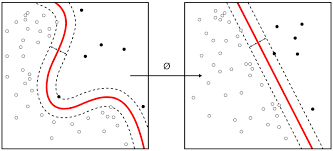
\includegraphics[scale=0.5]{figs/svm.png}
\caption[The case where classes aren't separable using linear boundary]{The left figure shows a case where the input data in their original space are not separable by a linear boundary. The right figure shows the same data transformed to a new space using a lifting function \o, and we can see that different classes are now separable  using linear boundary.}
%Source:
\label{fig:SVM_boundaries}
\end{figure}

A \emph{kernel method} consists in replacing every inner products $\mathbf{x}_i^T \mathbf{x}_j$ by a psd kernel $\mathcal{K}(\mathbf{x}_i, \mathbf{x}_j)$ during training, and similarly $\mathbf{x}_i^T\mathbf{x}$ by $\mathcal{K}(\mathbf{x}_i, \mathbf{x})$ during prediction.
Let us now explain the intuition behind this, starting by rewriting Eq. \ref{eq:inner_product} as 
\[
\hat{y}(\mathbf{x})=\text{sign}\{\textbf{x}^T(\mathbf{X}^T~diag([\alpha]_{i=1}^n)~\mathbf{Y})\},
\]
where $diag([\alpha]_{i=1}^n)$ is the diagonal matrix with values $[\alpha]_{i=1}^n$. \nt{**As $\mathbf{Y}$ is not really well defined, the reader, as it is, does not really understand the algebraic calculus at stake here**}

To get the decision boundary of such models we solve $\textbf{x}^T\textbf{q}=0$, where $\textbf{q}=(\mathbf{X}^T~diag([\alpha]_{i=1}^n)~\mathbf{Y})\in\mathbb{R}^d$. It is the equation of a hyper-plane in the input space $\mathbb{R}^d$, also referred to as a \emph{linear} decision boundary. 
The question here is: what if the the two classes are not separable by a hyper-plane (Fig. \ref{fig:SVM_boundaries})? 

One common solution to this problem is to map the data points from $\mathbb{R}^d$ to another space $\mathbb{R}^m$  through a proper mapping function \o~such \todoNK{Not fond of \o. How about $\varphi$ ?} \nt{I agree: $\varphi, \psi$?} that the two classes become separable with a linear decision boundary in $\mathbb{R}^m$. Then we can apply the same learning models specified in Eq. \ref{eq:inner_product} but on the transformed data. Let us consider for example the dataset shown in Fig. \ref{fig:polynomial_kernel},  we can use the following mapping function \o$:(x_1,x_2)\mapsto (\sqrt{2}x_1x_2,x_1^2,x_2^2)$ to move from $\mathbb{R}^2$ on the left, where data are not linearly separable, to $\mathbb{R}^3$ on the right, where they are.
\begin{figure}[H]
\centering
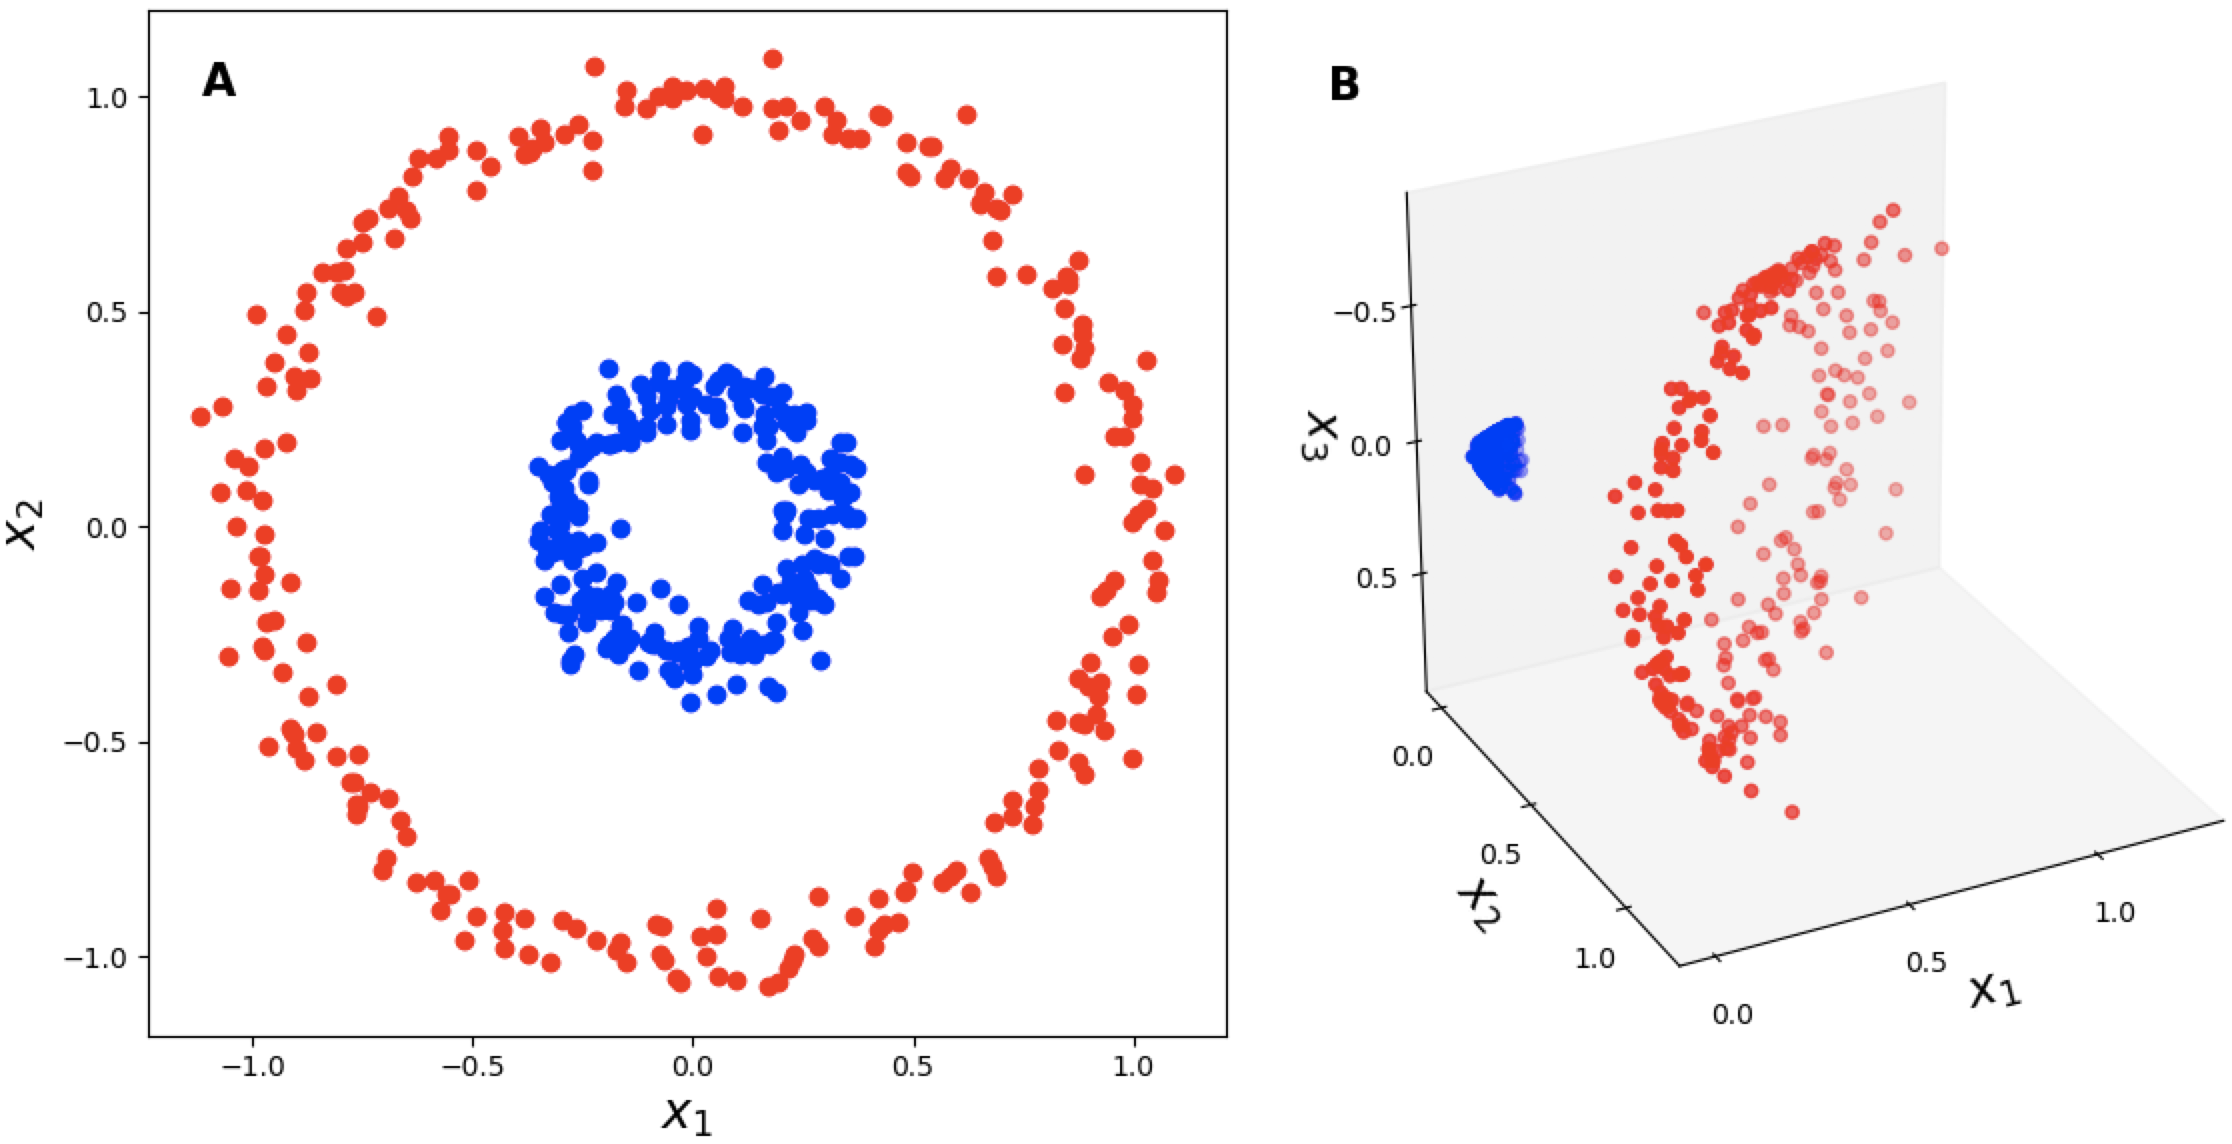
\includegraphics[scale=0.25]{figs/poly_kenrnel.png}
\caption[Lifting data to a higher-dimension space to get linearly separable classes]{ Using the mapping function \o$:(x_1,x_2)\mapsto (\sqrt{2}x_1x_2,x_1^2,x_2^2)$ to map the data on the left in $\mathbb{R}^2$ to $\mathbb{R}^3$ where they are linearly separable}
%Source:
\label{fig:polynomial_kernel}
\end{figure}
Learning such a function \o~is what is typically done by neural networks using complex optimization methods.  Kernel methods are much simpler (and elegant) methods to perform this mapping. They are justified by the following key theorem.
\begin{theorem}[Mercer theorem]
To every positive semi-definite kernel $\mathcal{K}:\mathbb{R}^d\times \mathbb{R}^d\mapsto \mathbb{R}$, there exists a Hilbert space $\mathbb{H}$ and a feature map $\phi:\mathbb{R}^d\mapsto\mathbb{H}$ such that for all $x,x'\in\mathbb{R}^d$ we have: 
\begin{equation}
\label{eq:kernel_main_equation}
    \mathcal{K}(\mathbf{x},\mathbf{x}')=<\phi(\mathbf{x}),\phi(\mathbf{x}')>_\mathbb{H}
\end{equation}
where $<\phi(\mathbf{x}),\phi(\mathbf{x}')>_\mathbb{H}$ is the inner product defined in $\mathbb{H}$.
\end{theorem}
This theorem states that replacing the inner product $\mathbf{x}_i^T\mathbf{x}$ in Eq. \ref{eq:inner_product} by a positive semi-definite kernel $\mathcal{K}(\mathbf{x}_i,\mathbf{x})$ is equivalent to implicitly map the data from the original input space $\mathcal{D}$ to another feature space $\mathbb{H}$ and then apply the classical inner product. Therefore, one \emph{does not need to know explicitely the mapping} $\phi$ nor the new feature space $\mathbb{H}$, instead, it is sufficient to evaluate the kernel $\mathcal{K}$ for pairs of data points in the original input space $\mathcal{D}$. This main feature of kernel methods is known as the \emph{kernel trick}. It has two main advantages:
\begin{itemize}
    \item Kernels allow us to transform data to a new Hilbert space of very high or even infinite dimensionality, which can make the learning model able to represent more complex functions.
    \item Kernels are often computationally cheaper, since they save the time required to compute the explicit co-ordinates of the data in the new feature space by directly calculating the inner product between the transformed data.
\end{itemize}
To better illustrate these benefits, we take the Gaussian kernel as an example, which is one of the most classical kernels in $\mathbb{R}^d$, defined as:
\begin{equation}
\label{eq:Guassian_kernel}
    \mathcal{K}_{G}(\mathbf{x},\mathbf{x}')=\exp^{-\frac{\left \| \mathbf{x}-\mathbf{x}'\right\|^2}{2\sigma^2}}
\end{equation}
where $\sigma>0$ is called the bandwidth parameter of the kernel. The lifting function $\phi_G$ of this kernel is located in a Hilbert space of infinite dimension, but the kernel can be easily evaluated for any pair $(\mathbf{x},\mathbf{x}')\in \mathcal{D}=\mathbb{R}^d$.

Despite their advantages, kernel methods still have some drawbacks:
\begin{itemize}
    \item Since for most kernels we need to evaluate the kernel on each pairs of data points, for a dataset $(\mathbf{X},\mathbf{X})$ \nt{?} of size $n$, we need $O(n^2)$ memory entries to compute what is called a Gram matrix, whose $(i,j)_{th}$ entry equals the kernel between points $\mathcal{K}(\mathbf{x_i}, \mathbf{x_j})$.
    \item Even if most kernels are designed so that they can be evaluated in polynomial time in the dimensionality of the input space $\mathcal{D}$ (for instance computing $\mathcal{K}_{G}(\mathbf{x},\mathbf{x}')$ for two vectors in $\mathbb{R}^d$ costs $d$ operations),  some kernels (especially on graphs) are computationally expensive \citep{graphlet_kernel}. \todoNK{I would not mention that here, since handling exponential computation of *each individual evaluation* of the kernel with RF is precisely what we do which has not been done before. Only the Gram matrix problem is mentioned in the original RF paper.}
\end{itemize}
To overcome these disadvantages, random feature projections is a technique developed to approximate kernels, often requiring less computational time and less memory storage.

\subsection{Random features}
Random features (RF) \citep{rahimi2008random} is an approach developed to approximate kernel methods with reduced computational time. The idea is that, instead of considering the true lifting function $\phi$ in Eq. \ref{eq:kernel_main_equation}, we explicitly map the data points using an appropriate randomized feature map $\varphi:\mathcal{D} \xrightarrow{}\mathbb{C}^m$, such that the kernel evaluated for two data points $x, x'$ is approximated by the inner product of their random features with high probability:
\begin{equation}
\label{eq:approx_RF}
\mathcal{K}(x,x')=<\phi(x),\phi(x')>_\mathbb{H} \approx \varphi(x)^*\varphi(x')
\end{equation}
Considering this approximation, we can transform the input with $\varphi$ and then apply a linear learning method as in Eq. \ref{eq:inner_product} to have a similar learning power as the original non-linear kernel machine, while often avoiding the cost of explicitely constructing the Gram matrix. Note that with RF we do not use the kernel trick anymore, but construct an explicit mapping $\varphi$ to approximate the kernel $\mathcal{K}$.

Most RF constructions are known as Random \emph{Fourier} Features (RFF), and are based on the following theorem.
\begin{theorem}[Bochner's theorem]
A continuous and shift-invariant kernel $\mathcal{K}(x,x')=\mathcal{K}(x-x')$ on $\mathbb{R}^d$ is positive definite if and only if $\mathcal{K}$ is the Fourier transform of a non-negative measure.
\end{theorem}
As a direct consequence, we can easily scale any shift-invariant kernel to obtain $\mathcal{K}(0) = \int p = 1$, so that its Fourier transform $p(w)$ is a correct probability distribution. We obtain that any shift-invariant psd kernel is of the form:
\begin{equation}
\label{Fourier integral}
\mathcal{K}(x-x')=\int_{\mathbb{R}^d}p(w)e^{jw^T(x-x')}dw= E_w[\xi_w(x)^*\xi_w(x')]
\end{equation}
where $\xi_w(x)=e^{-jw^Tx}$, where the expectation $E_w$ is over the appropriate probability distribution $p(w)$. Note that, since $\mathcal{K}$ is a real-valued function, from Eq.~\ref{Fourier integral} one can also prove that:
\begin{equation}
\label{real Fourier integral}
\mathcal{K}(x-x')=\int_{\mathbb{R}^d}p(w)cos({w^T(x-x')})dw=E_w[\tilde \xi_w(x)\tilde \xi_w(x')]
\end{equation}
where $\tilde \xi_w(x)=\sqrt{2}cos(w^Tx+b)$ such that $w$ is drawn from $p(w)$ and b is drawn uniformly from $[0,2\pi]$, so we can use real-valued mapping if desired.

As a result, for $w$ a random variable drawn from $p(w)$, $\ \xi_w(x)\xi_w(x')$ is an unbiased estimate of $\mathcal{K}(x,x')$. The RF methodology consists in averaging $m$ instances of the estimator with different random frequencies $w_j$ drawn identically and independently (iid) from $p(w)$, that is, define
\[
\varphi(x) = \frac{1}{\sqrt{m}} ( \xi_{w_j}(x) )_{j=1}^m \in \mathbb{C}^m
\]
such that $\varphi(x)^*\varphi(x')=\frac{1}{m} \sum_{j=1}^m \xi_{w_j}(x)^*\xi_{w_j}(x')$, which converges to $\mathcal{K}(x,x')$ by the law of large numbers. Moreover, Hoeffding's inequality guarantees exponentially fast convergence in $m$ between $\varphi(x)^*\varphi(x')$ and the kernel true value:
\begin{equation}
   \forall \epsilon >0\qquad Pr(|\varphi(x)^*\varphi(x')-\mathcal{K}(x,x')|\geq\epsilon)\leq2e^\frac{-m\epsilon^2}{4},
\end{equation}
that is, for any error $\epsilon$, the probability that the estimation is off by more than $\epsilon$ is controlled by an exponentially decaying term.

\nt{I would add here the theorem of the form (the union bound on the previous Hoeffding):
\begin{theorem}\label{thm:RF_vs_logn}
Let $\epsilon\in(0,1)$ and $\delta\in(0,1)$. Consider a dataset $\mathcal{X}=(\mathbf{x}_1,\ldots,\mathbf{x}_n)$ of $n$ elements, and a psd shift-invariant kernel $\kappa$. The random embedding  $\varphi(x)\in\mathbb{R}^m$ enables a controlled approximation of \emph{all} the elements of the Gram matrix with probability larger than $1-\delta$, \emph{i.e.}
$$\text{Pr}\left(\forall (\mathbf{x}, \mathbf{x}')\in\mathcal{X}^2\quad|\varphi(x)^*\varphi(x')-\mathcal{K}(x,x')|\leq\epsilon\right)\geq 1-\delta$$ 
provided that 
$$m\geq\mathcal{O}\left(\frac{1}{\epsilon^2}\log{\frac{n}{\delta}}\right).$$
\end{theorem}
I find this version useful as we clearly see that in fact random embedding is classically useful when $\log{n}\leq d$. If $d$ is too small, random embedding is in general useless. }

As an illustration, consider the Gaussian kernel in Eq. \ref{eq:Guassian_kernel} as an example. This kernel is shift-invariant and known to be positive semi-definite. It is already correctly normalized since $\mathcal{K}(0) = 1$, and its Fourier transform is a Gaussian probability distribution with inverted variance:
\[p(w)=FT\big(\mathcal{K}_G\big)(w)=\left(\frac{\sigma^2}{2\pi}\right)^\frac{d}{2}e^{-\frac{\sigma^2\|w\|^2}{2}}\]
Thus, in practice, in order to approximate the Gram matrix of $\mathcal{K}_G$ on a dataset $\mathcal{X}$ of size $n$, one i/~draws $m$ iid frequencies from this probability distribution, with $m$ as in Theorem~\ref{thm:RF_vs_logn}; ii/~uses these frequencies to associate to each element $x\in\mathcal{X}$ its associated random feature vector $\varphi(x)\in\mathbb{R}^m$; iii/~uses $\varphi(x)^*\varphi(x')$ as an approximation of $\kappa_G(\mathbf{x},\mathbf{x}')$ where necessary in any kernel-based learning algorithms.

\section{Graph kernels}

Kernel methods are a flexible set of tools, since psd kernels can be defined on any set of objects. Naturally, for machine learning tasks on graphs such as graph classification or regression, authors have developed kernels on graphs $\mathcal{K}(G,G')$ \citep{kriege_graph_kernels}. This section gives a brief overview of graph kernels, focusing on the so-called \emph{graphlet kernel}, which will be our main inspiration for this work. We start with a few definitions.

\subsection{Notations}

Recall that a graph $\mathcal{G} = (\mathcal{V}, \mathcal{E})$ is formed by a set of nodes and a set of edges connecting them. A graph $F=(\mathcal{V}_F,\mathcal{E}_F)$ is said to be a subgraph (also called \emph{graphlet}) of $\mathcal{G}$, written $F\sqsubseteq \mathcal{G}$, if and only if there exists an injective function $\mathcal{M}:\mathcal{V}_F\xrightarrow{} \mathcal{V}$ such that $(u,u')\in \mathcal{E}_F \Leftrightarrow{(\mathcal{M}(u),\mathcal{M}(u'))\in \mathcal{E}}$.

Any edge $(u_i, u_i)$ is called a self loop. In a general graph two vertices $u_i$ and $u_j$ may be connected by more than
one edge. A simple graph is a graph with no self loops or multiple edges. Here we always consider simple graphs.
A (simple) graph can equivalently be represented by an adjacency matrix $\mathbf{A}$ of size $v \times v$. The $(i,j)-th$ entry of $\mathbf{A}$ is 1 if an edge $(u_i, u_j)$ exists and zero otherwise.
Two graphs $\mathcal{G}=(\mathcal{V},\mathcal{E})$ and $\mathcal{G'}=(\mathcal{V'},\mathcal{E'})$ are said to be \emph{isomorphic}, written $\mathcal{G}'\cong \mathcal{G}$, if there exists a bijective function $\mathcal{M}:\mathcal{V}\xrightarrow{} \mathcal{V}'$ such that $(u_i,u_j)\in \mathcal{E}$ iff $(\mathcal{M}(u_i),\mathcal{M}(u_j))\in \mathcal{E}'$. Deciding is two graphs are isomorphic is known to be a difficult problem: it is actually an open question if this problem is solvable in polynomial time or is NP-complete.

\subsection{Convolutional graph kernels}

Recall that traditional kernel machines are applied to problems with vector-valued input data, where they compare different data points $x,x' \in \mathcal{R}^d$, often through their Euclidean distance. Based on that, these kernels cannot be used directly on (a vector representation of the) graphs: indeed, isomorphic graphs have different adjacency matrices but they represent the same structure. As a result it is necessary to measure distance between graphs in ways that are insensitive to isomorphism as well: ideally, if $\mathcal{G}_1 \cong \mathcal{G}'_1$ and $\mathcal{G}_2 \cong \mathcal{G}'_2$, then $\mathcal{K}(\mathcal{G}_1, \mathcal{G}_2)$ should be equal to, or at least very close to, $\mathcal{K}(\mathcal{G}_1, \mathcal{G}_2)$. One observes that the concept of isomorphism is critical in learning algorithms on graphs, not only because there is no known polynomial-time algorithm for testing graph isomorphism (except for graphs with specific structures), but simply testing isomorphism is also too strict for learning in a similar way to learning with equality operator \citep{kriege_graph_kernels}.

Since it is simpler to define kernels on \emph{small} graphs, most of the graph kernels in the literature belong to the family of \emph{convolution kernels}: given two graphs, the trick is to divide each into smaller subgraphs and then to pairwise compute a kernel between the resulted subgraphs.
\newtheorem{definition}{Definition} 
\begin{definition}[Convolution Kernel]
let $\mathcal{R}=\mathcal{R}_1\times...\times \mathcal{R}_d$ denote a space of components such that a composite object $X\in \mathcal{X}$ decomposes into elements of $\mathcal{R}$. Let $R:\mathcal{R}\xrightarrow{}\mathcal{X}$ denote the mapping from components to objects, such that $R(x)=X$ iff the components $x\in \mathcal{R}$ make up the object $X\in \mathcal{X}$, and let $R^{-1}(X)=\{x\in\mathcal{R}:R(x)=X\}$. then, the R-convolution kernel is:
\begin{equation}
\label{eq:conolutional_kernels}
    K_{CV}(X,Y)=\sum_{x\in R^{-1}(X)}~\sum_{y\in R^{-1}(Y)}~\underbrace{\prod_{i=1}^{d}k_i(x_i,y_i)}_{k(x,y)}
\end{equation}
with $k_i$ is a kernel on $\mathcal{R}$ for $i\in\{1,...,d\}$.
\end{definition}

Applying this definition on graphs, $R^{-1}(\mathcal{G}=(\mathcal{V},\mathcal{E}))$ includes all the components in graph $\mathcal{G}$  that we want to compare with the components $R^{-1}(\mathcal{G'}=(\mathcal{V}',\mathcal{E}'))$ in graph $\mathcal{G'}$. One example of these kernels is the node label kernel, where for two graphs $\mathcal{G}, \mathcal{G'}$, the mapping function $R$ maps the features $x_u\in \mathcal{R}$ of each node $u\in \mathcal{V}\cup \mathcal{V'}$ to the graph that $u$ is a member of. Another example, which will be our main source of inspiration and will be further described in the next section, is the $k$-graphlet kernel, where $R$ here maps the subgraphs of size $k$ to the graph in which they occur.
 
The advantage of using convolution kernel framework with graphs is that kernels are permutation invariant on the graphs level as long as they are permutation invariant on the components level. As a drawback, the sum in Eq.~\ref{eq:conolutional_kernels} iterates over every possible pair of components. As a result, when the base kernel has high value between a component and itself while it is low between two different components, each graph becomes drastically similar to itself but distant from any other graph. Thus, a set of weights is usually added to counter-balance this problem.

\subsection{Graphlet Kernel}
\label{subsection: graphlet kernel}

As mentioned above, the graphlet kernel is a special instance of convolution kernel equivalently described as follows: one enumerates all the subgraphs of size $k$ of each graph (where $k$ is small), counts them to build a histogram of their frequencies of apparition, and takes the inner product between the two histograms to obtain the final kernel. In this context, the subgraphs are called ``graphlets'', as an analogy with classical wavelets, which are individual components of more traditional signals.

Let us denote by $\mathcal{H}=\{\mathcal{H}_1,..., \mathcal{H}_{N_k}\}$ the set of all graphs of size $k$. Depending on the context, there is two choices in defining this set. Either we count all possible adjacency matrices and treat isomorphic graphs as different graphs, in which case we have $N_k=2^{k(k-1)/2}$ different graphlets. We refer to this case as graphlets \emph{with repetition}. Or we do not distinguish isomorphic graphs, so we have here $N_k<2^{k(k-1)/2}$ but it is still exponential in $k$. We call this case graphlets \emph{without repetition}. The classical graphlet kernel uses graphlets without repetition, which can require expensive isomorphism tests. We will see that some methods on graphlets \emph{with} repetition also perfom well in practice.

For either case, we define for a graph $\mathcal{G}$ the vector $f_\mathcal{G}\in \mathcal{R}^{N_k}$ whose $i$-th entry equals the normalized-number of occurrences of $\mathcal{H}_i$ in $\mathcal{G}$, that is $\#(\mathcal{H}_i\sqsubseteq G)/\tbinom{v}{k}$. The vector $f_G$ is usually referred to by the $k$-spectrum of G, and it is the key idea behind graphlet kernel. 
\begin{definition}[Graphlet Kernel]
Given two graphs $\mathcal{G}$ and $\mathcal{G}'$ of size $\geq k$, the graphlet kernel $\mathcal{K}_g$ is defined as \citep{graphlet_kernel}:
\begin{equation}
\label{eq:graphlet_kernel}
    \mathcal{K}_g(\mathcal{G},\mathcal{G}')=f_{\mathcal{G}}^Tf_{\mathcal{G}'}.
\end{equation}
where graphlets are taken without repetition.
\end{definition}
In this case the distance between graphs in the kernel space is just the Euclidean metric between histograms $d_\mathcal{K}({\mathcal{G}},{\mathcal{G}'}) = \|f_{\mathcal{G}} - f_{{\mathcal{G}'}}\|_2$.

The drawback of this kernel is that computing the $k$-spectrum vector costs huge computational time even for moderate $k$: there are $O\tbinom{v}{k}$ subgraphs of size $k$ in a graph of size $v$, the list of graphlets is of size $N_k$ exponential in $k$, and since graphlets are taken without repetition multiple isomorphism tests must be performed. As a result, there is a trade off between a more accurate representation of the graph (larger value of $k$) and the computational cost. However, some techniques are used in order to handle this limitation. In the next section, we focus on empirical sampling.

\subsection{Graph sampling to approximate k-graphlet spectrum}
\label{graph_sampling}
%Graph sampling arises when we deal with a large-scale graph and the task is to pick a small-size sample subgraph that would be similar to the original graph with respect to some important properties.

The graphlet kernel can be interpreted as follows: if one draws a subgraph randomly from $\mathcal{G}$, then one has a probability $(f_\mathcal{G})_i$ of obtaining $\mathcal{H}_i$. So, it is natural to approach $f_\mathcal{G}$ with an empirical histogram, built by  sampling $s$ subgraphs $F_1,...,F_s \sqsubseteq \mathcal{G}$ of size $k$, and then estimate the $k$-spectrum vector empirically: $(\hat f_\mathcal{G})_i = \frac{1}{s}\sum_{j=1}^s \mathbbm{1}[F_j \cong H_i]$. In other words, we count the number of times $\mathcal{H}_i$ appears among the samples. The Law of Large Numbers states that $\hat f_\mathcal{G} \xrightarrow[s \to \infty]{} f_\mathcal{G}$ with probability $1$.

This adds another degree of freedom to the method: there are many different ways of sampling a subgraph \citep{lescovec}, and each of them defines a different histogram $f_\mathcal{G}$ when $s \to \infty$. A \emph{sampling method} will be denoted by $S_k(\mathcal{G})$, it is a random variable that extracts a $k$-subgraph of $\mathcal{G}$. We describe two examples that we will use in the experiments.
\begin{itemize}
\item \textbf{Uniform sampling}: this is the simplest sampling method. We select a subset of $k$ nodes uniformly randomly among the $\tbinom{v}{k}$ possible choices, and extract the subgraph on these nodes. This is the sampling method that corresponds to the classical graphlet kernel \eqref{eq:graphlet_kernel} when $s \to \infty$.
\item \textbf{Random walk sampling}: todo

\end{itemize}




%\addchapheadtotoc
\chapter{Theoretical Analysis}
We recall that the majority of our work (especially the practical side) focus on using Random Features, mainly OPUs' light-speed random features, to approximate the graphlet kernel to approach Graph Classification problems. We also focus in some stage of this work on using Fourier Random Features to approximate the Gaussian kernel. Thus, in this chapter we first introduce the mathematical notions of Graph Kernels and Random Features. Then, we prove the efficiency of replacing the classical Graph Kernels which have two drawbacks (time, memory) by the use of their corresponding Random Features mapping function, this is to be done using concentration inequalities and information preservation concept. Finally, we show the structure of the OPU and its mathematical model. 

\section{Necessary Notations}
Before proceeding to the analysis of used methods, we first introduce the necessary notations related to Graph definition and Graph kernels.
A graph by definition is a pair $G=(V,E)$, where V is the set of the graph nodes (vertices) $V={v_1,...,v_n}$, and $E\in V\times V$ is the set of edges between these nodes, i.e. $(v_i, v_j)\in E$ means that the graph has an edge from node $v_i$ to node $v_j$ (or vice versa since we consider undirected graphs in this work).
\newline $H=(V_H,E_H)$ is said to be a subgraph (graphlet) of G ($H\sqsubseteq G$) if and only if there exist an injective function $\mathcal{M}:V_H\xrightarrow{} V$ such that $(v,w)\in E_H \Leftrightarrow{(\mathcal{M}(v),\mathcal{M}(w))\in E}$.\newline
Any edge $(v_i, v_i)$ is called a self loop. In a general graph two vertices $v_i$ and $v_j$ may be connected by more than
one edge. A simple graph is a graph with no self loops
or multiple edges. Here we always consider simple graphs.\newline
A simple graph can equivalently be represented by an adjacency matrix $A$ of size $n \times n$. The $(i,j)-th$ entry of $A$ is 1 if an edge $(v_i, v_j)$ exists and zero otherwise.\newline
Two graphs $G=(V,E)$ and $G'=(V',E')$ are isomorphic $(G'\cong G)$ if there exists a bijective function $\mathcal{M}:V\xrightarrow{} V'$ such that $(v_i,v_j)\in E$ iff $(\mathcal{M}(v_i),\mathcal{M}(v_j))\in E'$


\section{Graph Kernels}
The kernel trick is a way to generate features for algorithms that depend only on the inner product between pairs of input points. The mathematical basis behind it is that any positive definite function $k(x,y)$ with $x,y \in \mathcal{R}^d$ defines an inner product and a lifting function $\phi$ so that the inner product between lifted data points equals its kernel $<\phi(x),\phi(y)>=k(x,y)$. The convenience one gets deploying kernels-baed models is that there is no need to access the lifting function $\phi$, instead, the used algorithm accesses the data only through evaluations of $k(x,y)$. To better illustrate this benefit, we take the Gaussian Radial Basis function (RBF) kernel as an example, where:
\begin{equation}
    K_{RBF}(x,y)=exp(-\frac{\left \| x-y\right\|^2}{2\sigma^2})
\end{equation}
where $\sigma$ is called the bandwidth parameter of the kernel. The Hilbert space associated with the Gaussian RBF kernel has infinite dimension, but the kernel may be easily evaluated for any pair (x,y). 

\subsection{Graph kernels design}
Traditional kernel machines approach problems with vector-valued input data, where it compare different objects $(x,y \in \mathcal{R}^d)$ using the difference between vector components. Based on that, these kernels are imperfect to be used with graphs, since the structure of a graph is invariant to permutations of its representation (e.g. Adjacency matrix), i.e. the ordering by which nodes and edges are enumerated, which leads to isomorphic graphs, does not change the graph structure. So in this case distance-kernels between graph representation vectors are uninformative.As a result it is necessary to measure distance between graphs in ways that are themselves permutation invariant. While the concept of isomorphism is important in learning algorithms on graphs,  not only there is no known polynomial-time algorithm for testing graph isomorphism (except for graphs with specific structures), but isomorphism is also too strict for learning in a similar way to learning with equality operator \citep{kriege_graph_kernels}. \newline
The majority of kernels developed to solve graph learning problems are convolution kernels, where given two discrete structures (e.g., two graphs), the idea of convolution framework is to subdivide these to structures into sub-structures (nodes or subgraphs) and evaluate a kernel between each pair of such sub-structures. 
\newtheorem{definition}{Definition} 
\begin{definition}[Convolution Kernel]
let $\mathcal{R}=\mathcal{R}_1\times...\times \mathcal{R}_d$ denote a space of components such that a composite object $X\in \mathcal{X}$ decomposes into elements of $\mathcal{R}$. Let $R:\mathcal{R}\xrightarrow{}\mathcal{X}$ denote the mapping from components to objects, such that $R(x)=X$ iff the components $x\in \mathcal{R}$ make up the object $X\in \mathcal{X}$, and let $R^{-1}(X)=\{x\in\mathcal{R}:R(x)=X\}$. then, the R-convolution kernel is:
\begin{equation}
\label{eq:conolutional_kernels}
    K_{CV}(X,Y)=\sum_{x\in R^{-1}(X)}~\sum_{y\in R^{-1}(Y)}~\underbrace{\prod_{i=1}^{d}k_i(x_i,y_i)}_{k(x,y)}
\end{equation}
with $k_i$ is a kernel on $\mathcal{R}$ for $i\in\{1,...,d\}$.
\end{definition}

Projecting this definition on Graphs, the inverse map $R^{-1}(G)$ of the convolution kernel can be seen as the
set of all components of a graph G that we want to compare. An example of these kernels is the node label kernel whose mapping R takes the attributes $x_u\in \mathcal{R}$ of each node $u\in G\times H$ and maps them to the graph that u is a member of. The attractive advantage using convolution
kernel framework when working with graphs is that while the kernels on substructures are invariant to orderings of nodes and edges, so is the resulting graph kernel. On the other hand, the sum in Eq.~\ref{eq:conolutional_kernels} iterate over all pairs of components. When the considered components become more and more specific, each object becomes increasingly similar to itself, but no longer
to any other objects, this problem is called the diagonal dominance problem, since the entries on the main diagonal of the kernel matrix (Gram matrix) are much higher than other entries,Thus, weights between the components usually are added to balance Gram matrix entries so this drawback is resolved.


\subsection{Graphlet Kernel}
Referring by $\mathcal{G}=\{graphlet(1),..., graphlet(N_k)\}$ to the set of k-nodes graphlets, and considering a graph G of size n we can define a vector $f_G$ of length $N_k$ whose i-th component equals the normalized-number of occurrences of $graphlet(i)$ in G ($\#(graphlet(i)\sqsubseteq G)$. What should be noticed based on this definition is that no two different graphlets in $\mathcal{G}$ are isomorphic. $f_G$ is referred to by k-spectrum of G, and this vector is the key idea behind graphlet kernel. 


\begin{definition}[Graphlet Kernel]
Given two graphs $G$ and $G'$ of size $n,n'\geq k$, the graphlet kernel $k_g$ is defined as \citep{graphlet_kernel}:
\begin{equation}
    k_g(G,G')=f_G^Tf_G'.
\end{equation}
\end{definition}


The drawback of this kernel is that computing the k-spectrum vector costs a lot of computational time, since there are $\tbinom{n}{k}$ size-k subgraphs in a graph G of size n ($O(n^k) $ processing steps required), thus there is a trade off between a more accurate representation of the graph (large value of k) and the computational cost. However, some techniques are used in order to resolve this limitation as Sampling From Graph technique (section \ref{graph_sampling}).

\subsection{Graph Sampling to approximate k-Graphlet Spectrum}
\label{graph_sampling}
The problem of Graph Sampling arises when we deal with a large-scale graph and the task is to pick a small-size sample subgraph/s that would be similar to the original graph with respect to some important properties.\newline
Sampling from graph techniques are used to resolve the processing cost limitation of graphlet kernel, and it can deployed in two different manners:
\begin{enumerate} \itemsep0pt \parskip0pt \parsep0pt
    \item directly sample $m$ sugraphs $\{H_1,...,H_m\}$ of size k, and then estimate the k-spectrum vector empirically:
    $f_G(i)=\frac{1}{m}\Sigma_{j=1}^m \mathbbm{1}[H_j=graphlet(i)]$
    \item sample m subgraphs  $\{H_1,...,H_m\}$ of size $n'$ such that $n\gg n'>k$, then estimate $f_G$ as follows:
    $f_G=\frac{1}{m}\Sigma_{j=1}^m f_{H_j}$, this method is usually being referred to by Mean Kernel Method and is used in problems with large-scale or random distribution-based infinity-size graphs (see \ref{subsec:MMD}).
\end{enumerate}  
The important thing here is whether a sufficiently large number of random samples will lead to an empirical k-spectrum vector close to the actual vector. The number of samples needed to achieve a given confidence with a small probability of error is called the sample complexity. 
\newtheorem{theorem}{Theorem} 
\begin{theorem}
Let $f$ be a probability distribution on the
finite set $\mathcal{G}={g_1,...,g_a}$, $X={X_j}_{j=1}^m$ be a set of independent identically distributed (iid) random variables $X_j$ drawn from $f$, and $\hat{f}(g_i)=\frac{1}{m}\Sigma_{j=1}^m\mathbbm{1}(X_j=g_i)$. Then for a given $\epsilon>0$ and $\delta >0$ we have \citep{graphlet_kernel}:
\begin{equation}
m=\left \lceil \frac{2(log(2)a+log(\frac{1}{\delta} ))}{\epsilon^2} \right \rceil
\end{equation}
samples suffice to ensure that $P\{\left\| f-\hat{f} \right\|_1 \geq \epsilon \}\leq\delta$
\end{theorem}
Therefore this theorem gives a lower bound on the number of samples considered respecting the first manner using Graph Sampling to approximate the k-Graphlet spectrum vector in order to ensure some certainty $\epsilon$ with prabability $(1-\delta)$.
\section{Random Features}
Kernel machines are of interest as they approximate any function arbitrarily well with sufficiently large training data set. On the other hand, the methods that operate on the kernel matrix (Gram matrix) require a lot of time in order to compute this matrix and to train the machine; for example, a dataset with half a million training examples might take days to train on modern workstations \citep{rahimi2008random}.
Unlike kernel machines, linear support vector machines and regularized regression run much faster especially with low-dimensionality training data. 
One way to combine the advantages of the linear and nonlinear vector machines is to convert the training and evaluation of any kernel machine into the corresponding operations of a linear machine by mapping data into a relatively low-dimensional randomized feature space.
Instead of considering the implicit lifting function which corresponds to the kernel, it was proposed to explicitly map the data to a low-dimensional Euclidean inner product space using a randomized feature map $z:\mathcal{R}^d \xrightarrow{}\mathcal{R}^D$ so that the inner product between a pair of transformed points approximates their kernel:
\begin{equation}
\label{eq:approx_RF}
k(x,y)=<\phi(x),\phi(y)> \approx z(x)^Tz(y)
\end{equation}
Considering this approximation, we can simply transform the input with $z$ and then apply a fast linear learning method to approximate the answer of the real kernel. \newline
In what follows, Random Fourier Features method to construct the random feature map function $z$ is presented.

\subsection{Random Fourier Features}
The following Theorem represents the key idea behind this mapping technique
%\newtheorem{theorem}{Theorem}
\begin{theorem}[Bochner's theorem]
A continuous and shift-invariant kernel $k(x,y)=k(x-y$ on $\mathcal{R}^d$ is positive definite if and only if $k(\delta)$ is the Fourier transform of a non-negative measure.
\end{theorem}
What that means is that when a shift-invariant kernel $k$ is properly scaled, its Fourier transform $p(w)$ is a proper probability distribution, we can write:
\begin{equation}
\label{Fourier integral}
k(x-y)=\int_{\mathcal{R}^d}p(w)e^{j{w}'(x-y)}dw=E_w[e^{j{w}'x}{e^{j{w}'y}}^*]
\end{equation}
But both $p(w)$ and $k(\delta)$ are real-valued functions, thus from Eq.~\ref{Fourier integral} we can prove that:
\begin{equation}
\label{real Fourier integral}
k(x-y)=\int_{\mathcal{R}^d}p(w)cos({{w}'(x-y)})dw=E_w[z_w(x)z_w(y)]
\end{equation}
where $z_w(x)=\sqrt{2}cos({w}'x+b)$ such that $w$ is drawn from $p(w)$ and b is drawn uniformly from $[0,2\pi]$.\newline
As a straight result, $\ z_w(x)z_w(y)$ is an unbiased estimate of k(x,y). We can achieve lower variance estimation to the expectation (Eq. \ref{real Fourier integral}) by averaging $D$ instances of the estimator with different random frequencies $w$. i.e. the low-variance estimator can be written as: $z(x)'z(y)=\frac{1}{D} \Sigma_{j=1}^D z_{w_j}(x)z_{w_j}(y)$. this estimator and based on Hoeffding's inequality guarantees exponentially fast convergence in $D$ between $z(x)'z(y)$ and the kernel true value:
\begin{equation}
    Pr(|z(x)'z(y)-k(x,y)|\geq\epsilon)\leq2e^\frac{-D\epsilon^2}{4}
\end{equation}

\subsection{Random features from compressed sensing's  point of view}
Random features can be tackled within a different paradigm in signal processing, in compressed sensing for instance a random projection of a high-dimensional but sparse or compressible signal onto a lower-dimensional space has been shown to contain enough information to be used to reconstruct the original signal with small error margins. In this domain, the well-known Johnson-Lindernstrauss (JL) lemma states that with high probability the geometry of a point cloud is preserved by certain Lipschitz mapping onto a space of dimension logarithmic in the number of points, and with the help of concentration inequalities for random inner products more efficient algorithms for constructing such embeddings were developed. First, we recall $\ell_p^N$ norm of a vector $x\in\mathcal{R}^N$:
\begin{equation}
    \left \| x\right\|_{\ell_p^N}=
    \left\{\begin{matrix}
{(\Sigma_{i=1}^N x_i^p)}^\frac{1}{p}\qquad,  0<p<\infty\\ 
max_{i=1,...,N}\left \| x_i\right\|~~\quad, p=\infty
\end{matrix}\right.
\end{equation}
In the discrete compressed sensing, we want to economically record information about a vector $x\in \mathcal{R}^N$, thus we allocate a group of n nonadaptive questions to ask about $x$. Each question takes the form of a linear function applied to $x$, i.e. the extracted information can be written in the form: 
\begin{equation}
    y=\phi x
\end{equation}
where $\phi \in \mathcal{R}^{n\times N}$ and $n$ is much smaller than $N$. \newline
To reconstruct the original signal from the information that $y$ holds about $x$, a decoder $\Delta$ is used to provide an approximation $\bar{x}=\Delta(y)=\Delta(\phi x)$. It should be noticed in our case with graph classification problem using random features that it is not one of our concerns to find or prove the proficiency of any decoder, but it is important to cover the mathematics that prove the efficiency of random projections represented in compressed sensing by the pair $(\phi, \Delta)$ . to measure the performance of an encoder-decoder pair $(\phi, \Delta)$, we use a norm $\left\| .\right\|_X$ to quantify the error: 
\begin{equation}
    e(x,\phi,\Delta)_X=\left\| x-\Delta(\phi x)\right\|_X
\end{equation}
which is the error of the pair $(\phi, \Delta)$ on $x$. Moreover, if K is any compact set in $\mathcal{R}^N$, then the error of this pair on K is:
\begin{equation}
    e(K,\phi,\Delta)_X = \underset{x\in K}{sup} ~e(x,\phi,\Delta)_X
\end{equation}
To find the best pair that minimizes the previous error, we introduce the set $\mathcal{A}_{n,N}=\{(\phi, \Delta ): \phi \in \mathcal{R}^{n\times N}\}$, thus the best performance of such pair on $K$ is given by: 
\begin{equation}
e_{n,N}(K)_X= \underset{(\phi, \Delta)\in \mathcal{A}_{n,N}}{inf}~e(K,\phi,\Delta)_X
\end{equation}
However, it was proven that if $K\subset \mathcal{R}^N$ such that $K=-K$ and that $K+K\subset C_1K$ ,where $C_1$ is a constant, then\citep{concentration_kashin}:
\begin{equation}
\label{3.5}
   d^n(K)_X < e_{n,N}(K)_X<C_1d^n(K)_X
\end{equation}
where $d^n(K)_X$ is Gelfand width of $K$ in the Banach space $X$:
\begin{equation}
    d^n(K)_X= \underset{codim(Y)=n}{inf}~\underset{x\in K\cap Y}{sup}\left\|x\right\|_X
\end{equation}
Here the best spaces $Y$ are those that slice through $K$ in the most economical direction to minimize the diameter of the set $K\cap Y$ (which corresponds to the direction with minimum variance notion used in Principle Component Analysis PCA). An important result of Gelfand widths that can be used in our paradigm is the limits of this width on the unit ball $K=U(\ell_1^N)$, it states that there exists a constant $C_0>0$ such that the following condition is satisfied whenever $0< n< N $:
\begin{equation}
    C_0^{-1}\sqrt{\frac{log(N/n)+1}{n}}\leq d^n(U(\ell_1^N))_{\ell_2^N}\leq C_0\sqrt{\frac{log(N/n)+1}{n}}
\end{equation}
Back to the proof of Eq.~\ref{3.5} Which can be done by checking the correspondence between $Y$ and $\phi$, where given any matrix $\phi$, its null space $\mathcal{N}$ is a valid candidate for $Y$ in computing $d^n(K)_X$. On the other hand, given any $Y$ of co-dimension $n$ used in computing $d^n(K)_X$, any basis for the orthogonal complement of $Y$ can be used as the rows of a matrix $\phi$ to estimate $E_{n,N}(K)_X$. For example, the unit ball $U(\ell_1^N)$ in $\ell_2^N$ satisfies that $U(\ell_1^N)+U(\ell_1^N)\subset 2U(\ell_1^N)$, thus for all $0< n< N$ : 
\begin{equation}
\label{3.6}
    C_0^{-1}\sqrt{\frac{log(N/n)+1}{n}}\leq E_{n,N}(U(\ell_1^N))_{\ell_2^N}\leq 2C_0\sqrt{\frac{log(N/n)+1}{n}}
\end{equation}
The main problem then is to find the pair $(\phi, \Delta)$ which provides estimates like Eq.~ \ref{3.6}, to address this question an isometry condition on $\phi$ was introduced. Given a matrix $\phi$ and any set T of column indices, we refer by $\phi_T$ to the $n\times \#(T)$ matrix composed of these columns. Simultaneously, for every $x\in \mathcal{R}^N$, we refer by $x_T$ to the vector obtained by considering only the entries in $x$ which correspond to the column indices $T$. We say that a matrix $\phi$ satisfies the RIP (Ristricted Isometry Property) of order k if there exists a $\delta_k\in [0,1]$ such that:
\begin{equation}
    \label{3.8}
    (1-\delta_k)\left\|x_T\right\|_{\ell_2^N}^2\leq
    \left\|\phi_Tx_T\right\|_{\ell_2^N}^2\leq  (1+\delta_k)\left\|x_T\right\|_{\ell_2^N}^2
\end{equation}
holds for every such set $T$ with $\#T\leq k$. The good matrices $\phi$ should satisfy the RIP condition for the largest possible $k$. For instance, if $\phi$ satisfies the RIP of order $3k$ with $\delta_{3k}<1$, then:
\begin{equation}
\label{3.9}
\left\|x-\Delta(\phi x)\right\|\leq \frac{c_2\sigma_k(x)_{\ell_1^N}}{\sqrt(k)}
\end{equation}
where $\sigma_k(x)_{\ell_1^N}$ is the $\ell_1$ error of the best k-term approximation and the constant $C_2$ depends only on $\delta_{3k}$. Since $\sigma_k(x)_{\ell_1^N}\leq \left\|x\right\|_{\ell_1^N}$ , we can obtain the best possible performance correspondent to Eq.\ref{3.6} if we can find a matrix $\phi$ that meet the RIP condition for $k$ of order $n/(log(N/n)+1)$.\newline
Now the question is how to construct such matrix $\phi$ that satisfy the RIP for the largest possible range of $k$. Actually, the only known constructions yielding such matrices are based on random matrices \citep{concentration_kashin}. It is shown that matrices built using random entries drawn from certain probability distributions will meet the RIP Condition with high probability. More specifically, for these constructions of $\phi$, the RIP follows in a simple way from the same concentration of measure inequalities for inner products that have employed to prove the JL lemma (which will not be stated here being irrelevant). \newline
Briefly, it is shown \citep{concentration_achlioptas} that any random variable which satisfies certain moment conditions, the matrix $\phi$ whose entries are independent realizations of this variable can be proven to satisfy the following concentration inequality for any $\epsilon \in [0,1]$:
\begin{equation}
\label{4.3}
    Pr(|~ \left\| \phi x\right\|_{\ell_2^N}^2- \left\|x \right\|_{\ell_2^N}^2~|\geq \epsilon\left\| x\right\|_{\ell_2^N}^2 )\leq 2e^{-nc_0(\epsilon)}
\end{equation}
Where $c_0(\epsilon)$ is only a function of $\epsilon$. The point now is to prove satisfying Eq.\ref{4.3} with some covering arguments is sufficient to prove the RIP for the corresponding matrix $\phi$, then some examples of these distributions are presented.
Considering the same aforementioned notation $\phi_T, X_T$ with $\#T\leq k$ with $\ell_2$ norm, the proof includes constructing  nets of points in each k-dimensional subspace, apply \ref{4.3} to all of these points through a union bound, and then extend the result from our finite set of points to all possible k-dimensional signals. 
\newtheorem{lemma}{Lemma} 
\begin{lemma}
let $\phi(w), w\in \omega^{n\times N}$, be  a random matrix of size $n\times N$ drawn from any distribution that satisfies the concentration inequality (\ref{4.3}). Then, for any set T with $\#T= k<n$ and any $0< \delta< 1$, we have
\begin{equation}
(1-\delta) \| x\|_{\ell_2^N}  
\leq
\| \phi(w)x\|_{\ell_2^N} 
\leq
(1_+\delta) \| x\|_{\ell_2^N} ~for ~all ~x\in X_T
\label{5.1}
\end{equation}
with probability
\begin{equation}
\geq 1-2(12/\delta)^k e^{-c_0(\delta/2)n}
\label{5.2}
\end{equation}

\end{lemma}

The first step of the proof is noticing that since $\phi$ represents a linear transformation, it is enough to prove \ref{5.1} in the case $\|x\|_{\ell_2^N}=1$. The next step is to choose a finite set of points $Q_T\subset X_T$ with $\|q\|_{\ell_2^N}=1$ for all $q\in Q_T$, that satisfies:
\begin{equation}
    \underset{q\in Q_T}{min}~ \|x-q\|_{\ell_2^N}\leq\delta/4 ~~for ~all ~x\in X_T
\end{equation}
The existence of such group is proven within the scope of covering numbers where also we can find that $\#Q_T\leq (12/\delta)^k$. Now, using the union bound to apply \ref{4.3} to this $Q_T$ with $\epsilon=\delta/2$, with
probability exceeding the right side of \ref{5.2}, we have:
\begin{equation}
(1-\delta/2) \| q\|_{\ell_2^N}  
\leq
\| \phi(w)q\|_{\ell_2^N} 
\leq
(1+\delta/2) \| q\|_{\ell_2^N} ~for ~all ~q\in Q_T
\end{equation}
Let A be the smallest number such that:
\begin{equation}
     \| \phi(w)x\|_{\ell_2^N} \leq (1+A) \| x\|_{\ell_2^N} ~for ~all ~x\in X_T
\label{5.6}
\end{equation}
But there is $q\in Q_T$ such that $\| x-q\|_{\ell_2^N}\leq \delta/4 $, so we have:
\begin{equation}
    \| \phi(w)x\|_{\ell_2^N} \leq
    \| \phi(w)q\|_{\ell_2^N} +
    \| \phi(w)(x-q)\|_{\ell_2^N} \leq
    1+\delta/2 +(1+A)\delta/4
    \label{5.7}
\end{equation}
By a simple comparison between Eq.\ref{5.6} and Eq. \ref{5.7}, we get that $A\leq \delta$, which is what we seek proving the upper inequality in Eq. \ref{5.1}, and the lower one can be proven in a similar way.
\begin{theorem}
when n<N, and $0< \delta< 1$,  If the probability distribution generating the $n\times N$ matrices $\phi(w), w\in \Omega^{n\times N}$, satisfies the concentration inequality \ref{4.3}, then there exist constants $c_1, c_2> 0$ depending only on $\delta$ such that
the RIP condition holds for $\phi(w)$ with the prescribed $\delta$ and any $k \leq c_1n/log(N/k)$ with probability $\leq 1-2e^{-c_2n}$.
\end{theorem}
To prove this theorem, from Eq.\ref{5.1} we know that the matrix $\phi(w)$ doesn't satisfy the inequality with probability $\leq 2(12/\delta)^ke^{-c_0(\delta/2)n}$ for each of the k-dimensional sub-spaces. But there are $\binom{N}{k}\leq (eN/k)^k$ such sub-spaces. Thus, this probability for all the sub-spaces becomes: 
\begin{equation}
    \leq  2(eN/k)^k(12/\delta)^ke^{-c_0(\delta/2)n}=2e^{-c_0(\delta/2)n+k[log(12/\delta)+log((eN/k))]}
\label{5.10}
\end{equation}{}
So for a fixed $c_1>0$, and $k\leq c_1n/log(N/k) $, we have that the exponent in Eq. \ref{5.10} is $\leq -c_2n$ provided that $c_2\leq c_0(\delta/2)-c_1[1+(1+log(12/\delta))/log(N/k)]$. Hence, when $c_1>0$ is sufficiently small we have $c_2>0$. So this is what we seek, This proves that with probability $1-2e^{-c_2n}$, the matrix $\phi(w)$ will satisfy Eq. \ref{5.1} on all the k-dimensional sub-spaces for the range of $k\leq c_1' n/[log(N/n) + 1]$ for $c_1'$ depending only on the aforementioned $c_1$.\newline 
The main example of such distributions that satisfy the inequality in \eqref{4.3} (so the moments of it satisfy the prerequisites of this inequality)  is the random matrix $\phi$ whose entries are independent realizations of Gaussian random variable \citep{concentration_kashin}:
\begin{equation}
    \phi_{i,j}\sim \mathcal{N}(0,\frac{1}{n})
\end{equation}
Where the corresponding constant $c_0$ is $c_0(\epsilon)=\epsilon^2/4-\epsilon^3/6$.
Another two examples related to Bernouli distribution which has the same value of the constant $c_0(\epsilon)$:
\begin{equation}
    \phi_{i,j}= 
    \left\{\begin{matrix}
    +1/\sqrt{n} ~ with ~probability ~\frac{1}{2}
\\ 
-1/\sqrt{n} ~ with ~probability ~\frac{1}{2}
\end{matrix}\right.
\end{equation}

\begin{equation}
    \phi_{i,j}= 
    \left\{\begin{matrix}
    +\sqrt{3/n} ~ with ~probability ~\frac{1}{6}
\\ 
0 ~ with ~probability ~\frac{2}{3}
\\
 -\sqrt{3/n} ~ with ~probability ~\frac{1}{6}

\end{matrix}\right.
\end{equation}


\subsection{Mean kernel and random features} \label{subsec:MMD}
%\paragraph{Mean kernel and MMD} 
The mean kernel methodology allows to \emph{lift} a kernel from a domain $\mathcal{X}$ to a kernel on \emph{probability distributions} on $\mathcal{X}$. Given a base kernel $k$ and two probability distribution $P,Q$, it is defined as
\begin{equation}\label{eq:mean_kernel}
k(P,Q) = \mathbb{E}_{x \sim P, y \sim Q} k(x,y)
\end{equation}
In other words, the mean kernel is just the expectation of the base kernel with respect to each term. The associated Euclidean metric is referred to by the  \emph{Maximum Mean Discrepancy (MMD)}, and is naturally defined as:
\begin{equation}\label{eq:MMD}
MMD(P,Q) = \sqrt{k(P,P) + k(Q,Q) - 2k(P,Q)}
\end{equation}
It should be noticed here that $k(P,P) = \mathbb{E}_{x \sim P, x' \sim P} k(x,x') \neq \mathbb{E}_{x \sim P} k(x,x)$.
NOw given data points $(x_1, \ldots, x_n)$ drawn $iid$ from $P$ and $(y_1, \ldots, y_n)$ drawn $iid$ from $Q$, the kernel in Eq. \ref{eq:mean_kernel} can naturally be approximated by:
\begin{equation}\label{eq:mean_kernel_approx}
k(P,Q) \approx \frac{1}{n^2} \sum_{i,j=1}^n k(x_i,y_j)
\end{equation}
and the corresponding approximate MMD is (other variants exist):
\[
MMD(P,Q) \approx \sqrt{\frac{1}{n^2} \sum_{i,j=1}^n k(x_i,x_j) + k(y_i,y_j) - k(x_i,y_j) - k(x_j, y_i)}
\]

\paragraph{MMD and random features}
Mean kernel works especially well with random features. Combining \eqref{eq:approx_RF} and \eqref{eq:mean_kernel_approx}, it is not hard to see that using random features the mean kernel can be further approximated by:
\begin{equation}
\label{eq:mean_kernel_RF}
k(P,Q) \approx \frac{1}{n^2} \sum_{i,j=1}^n \phi(x_i)^*\phi(y_j) = \left(\frac{1}{n} \sum_i \phi(x_i)\right)^* \left(\frac{1}{n} \sum_i \phi(y_i)\right)
\end{equation}
So the computation can be drastically improved by first computing the \emph{averaged random features} (also called random \emph{generalized moments}, also called \emph{sketch}) $\frac{1}{n} \sum_i \phi(x_i)$, and taking a linear kernel between them. The corresponding MMD is then just the Euclidean metric between the averaged random features
\[
MMD(P,Q) \approx \| \frac{1}{n} \sum_i \phi(x_i) - \frac{1}{n} \sum_i \phi(y_i)\|_2
\]

\paragraph{MMD for discrete distributions}
for a discrete space of objects $H_1, \ldots, H_N$ with discrete probability distributions $P = [P_1, \ldots, P_N]$ and $Q$ on them, the mean kernel \ref{eq:mean_kernel} takes a particular form:
\[
k(P,Q) = \sum_{i,j=1}^N P_i Q_j k(H_i, H_j)
\]

\paragraph{MMD with random features on discrete distrbutions}

To combine both notions One can see the link with graphlet sampling, where $f_G$ is the (discrete) probability distribution of the graphlets. If we define $k(F, F') \approx \phi(F)^*\phi(F')$ where $\phi$ is a random feature map that replaces $\phi_k$, then the feature map \eqref{eq:graphlet_kernel_approx} is exactly what appears in \eqref{eq:mean_kernel_RF}. So, now, all the game becomes to find a good feature map $\phi(F)$ for graphlets. The induced MMD metric between graphs is the MMD between graphlets probability distributions $f_G$:
\[
d(G,G') = MMD(f_G, f_{G'}) = \sqrt{k(f_G, f_{G}) + k(f_{G'}, f_{G'}) - 2 k(f_G, f_{G'})} \approx \| \frac{1}{n} \sum_i \phi(F_i) - \frac{1}{n} \sum_i \phi(F'_i)\|_2
\]
where $F_i$ are graphlets drawn from $G$ and $F'_i$ are graphlets drawn from $G'$.






\section{Random Projections with Optical Processing Units (OPU's)}
Random projections is one of the important techniques in machine learning and signal processing, but it requires either to store a very large random matrix, or to use a
different, structured matrix to reduce the computational and memory costs. Optical processing units (OPU's) are the tools used to overcome this difficulty, an OPU performs random projections at the speed of light without having to store any matrix in memory. In general, Random projections are the result of two procedures where the first one is the linear-random projections and the second one is non-linear mapping.
Mathematically speaking, OPU's perform the following operation \citep{saade_opu}:
\begin{equation}
\label{OPU_equation}
    X=\phi(WU+b);~W\in \mathcal{R}^{r\times d},b\in \mathcal{R}^r, U\in \mathcal{R}^d
\end{equation}
where $W$ is the random projection matrix, b is a bias, U is an input point, r is the number of random features and d is the input space dimension.With, $W$ is a random i.i.d complex matrix with Gaussian real and imaginary parts and $\phi$ is the non-linear mapping function.\newline
In the limit where the number of random features $r\xrightarrow{}\infty$, it can be proven by the concentration of the measure that the inner product between the projected data points $(X_i\in \mathcal{R}^r)$ in the new feature space tends to a kernel function that depends only on the input points in the original feature space $(U_i\in \mathcal{R}^d)$

\subsection{OPU structure and functionality}
Eq.~\ref{OPU_equation} still imply that an OPU need to store and multiply by the random projection matrix.\newline
In such units a heterogeneous material, such as paper or any white translucid material, is used to scatter incident light in a very complex way, so the behavior of light scattering is considered random because of the extremely high complexity. one can argue that light scattering is a linear, deterministic, and reproducible phenomenon, but what can be said is that the unpredictable nature of the process makes it effectively a random process, that is why these materials are called opaque since all information carried within the incident light is seemingly lost during the propagation through the material \citep{saade_opu}. An example used to demonstrate and justify the resulted randomness is a cube of edge length $100\mu m$, such cube can comprise $\approx 10^7$ paint nanoparticles, all the positions and shape of these particles must be known in order to predict its effect on light. Propagation through such a layer can be seen as a random walk because of frequent scattering with the nanoparticles, where light would explore the whole volume
and endure on average tens of thousands of such scattering steps before exiting on the other side in a few picoseconds.\newline

\begin{figure}[ht!]
\begin{center}
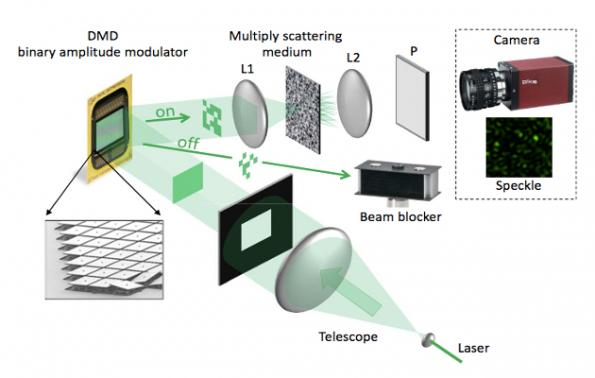
\includegraphics[scale=0.5]{figs/lighton630.jpg}
\end{center}
\caption[OPU's Experimental setup]{OPU's Experimental setup \citep{saade_opu}: A monochromatic laser is expanded by a telescope, then
illuminates a digital micromirror device (DMD), able to spatially encode digital information on the light beam by
amplitude modulation. The light beam carrying the signal is then focused on a random
medium by means of a lens. The transmitted light is collected on the
far side by a second lens, passes through a polarizer, and is measured by a standard monochrome CCD camera for example .}


\label{fig_opu}
\end{figure}


When the incident light is coherent, it gives rise to interferences, and the complex interference pattern arising from the multiple scattering process is called speckle. These patterns are not characteristic only of the propagation medium but also of the shape of the incident light, and this can be modeled by $y=Wx$, where y and x are the vector amplitudes between a set of spatial modes at the output and at the input of the medium respectively and $W$ is the transmission matrix of the medium and it was shown to be very close to Gaussian i.i.d matrices \citep{saade_opu}. What's more convenient to use the aforementioned configuration as a platform for random projections, even without W being determined, is that for a stable medium, such as a paint layer, the transmission matrix $W$ is stable as well. 
So lightening this layer with an appropriate set of incident illuminations, which is possible using a spatial light modulator and a laser, and measuring the output speckle using CCD or CMOS camera, we can record the resulting intensity $|y|^2$, which is the principle concept behind OPU's functionality as seen in Fig~ \ref{fig_opu}.\newline
The DMD (digital micromirror device) used in OPU's is a Binary Amplitude Modulator consisting of an array of micro-mirrors, Each encodes a binary value(lit or not). In order to represent grey values, each value is encoded on a square sub-array ($4\times 4$ for example) in the DMD,where the number of lit mirrors reflects the desired level of grey. DMD reflects the data through the disordered medium, and a snapshot of the resulting random projection is acquired using a standard camera, all that in a very high speed compared to the traditional random features techniques. 



\iffalse
Example of double quotes ``word''. Lorem ipsum dolor sit amet, consectetur adipiscing elit. Curabitur viverra, velit eget vestibulum viverra, nisl eros aliquet sapien, sed interdum tellus justo et purus. Nulla vel orci nisl. Curabitur porta lacinia quam, finibus bibendum mi tincidunt eget. Aenean aliquam lobortis orci, ut aliquam neque imperdiet vel. Nunc sit amet scelerisque velit. Aenean quis tempor leo, at consectetur ipsum. Nam ac urna dapibus, condimentum orci a, ornare ante. In hac habitasse platea dictumst. 
\subsection{Another subsection of section - citations}
Example of citation \citep{altschul1997gapped}. Mauris nisi felis, pharetra vitae velit at, sollicitudin molestie justo. Aenean tristique diam pulvinar, semper risus sed, mattis elit. Phasellus interdum erat at enim maximus interdum. Curabitur tempor, arcu nec malesuada facilisis, tortor nisi ornare ex, ut porttitor elit lectus aliquam diam. Cum sociis natoque penatibus et magnis dis parturient montes, nascetur ridiculus mus. Vivamus quam turpis, auctor in nunc nec, varius pharetra nibh. Ut sagittis diam nec dui sodales tempor. Integer molestie diam id quam placerat eleifend. Nulla posuere iaculis nisi, et sagittis ipsum consequat scelerisque. In nec turpis eget tellus pulvinar porttitor vitae ac tortor. Nullam tempor ut orci ac porttitor. Pellentesque aliquam lacinia gravida. Duis accumsan tristique augue, vitae aliquam magna convallis ac. Aenean vel diam non eros venenatis ullamcorper sit amet at augue. 


Example of multiple citations \citep{altschul1997gapped,baker2007novel}. Nullam mollis et leo at pharetra. Nulla efficitur molestie euismod. Sed dapibus metus sed tempus varius. Aenean finibus eros ut urna luctus feugiat. Duis turpis risus, viverra vitae porta et, ullamcorper ac est. Proin in eros nec ipsum interdum tempus. Nam fringilla lectus velit, non posuere ex vehicula ut. Mauris tincidunt, dolor sit amet commodo tempor, erat mi egestas dui, at elementum tellus est rhoncus libero. Ut et rutrum lectus, id viverra tortor. Vivamus nec lacus eros. Donec dictum porta nisi et vestibulum. Mauris luctus ligula ut libero aliquet luctus. Quisque malesuada egestas finibus. 
\subsubsection{Subsubsection of section - italic text}
Example of italic text - {\it Escherichia}, {\it Salmonella}, and {\it Shigella} spp. Mauris dictum pharetra fermentum. Maecenas ut felis varius, dapibus sapien imperdiet, dictum dui. Proin feugiat viverra metus non laoreet. Integer pulvinar mi id lacus semper commodo. Praesent vel erat interdum purus scelerisque maximus. Sed enim risus, mollis blandit ligula ac, sagittis venenatis augue. Mauris nisi purus, gravida ac aliquam eu, ullamcorper eget nulla. Proin id finibus purus. Vestibulum leo ante, porta in quam sed, eleifend feugiat arcu. Nunc viverra fringilla turpis a iaculis. In condimentum aliquet mauris, quis laoreet eros porta eu. Aenean ut turpis a massa gravida pretium. Phasellus auctor purus quis diam interdum, nec luctus lorem auctor. Pellentesque finibus elit justo, a vulputate diam fermentum lacinia. 
\section{Another section}
Mauris dictum pharetra fermentum. Maecenas ut felis varius, dapibus sapien imperdiet, dictum dui. Proin feugiat viverra metus non laoreet. Integer pulvinar mi id lacus semper commodo. Praesent vel erat interdum purus scelerisque maximus. Sed enim risus, mollis blandit ligula ac, sagittis venenatis augue. Mauris nisi purus, gravida ac aliquam eu, ullamcorper eget nulla. Proin id finibus purus. Vestibulum leo ante, porta in quam sed, eleifend feugiat arcu. Nunc viverra fringilla turpis a iaculis. In condimentum aliquet mauris, quis laoreet eros porta eu. Aenean ut turpis a massa gravida pretium. Phasellus auctor purus quis diam interdum, nec luctus lorem auctor. Pellentesque finibus elit justo, a vulputate diam fermentum lacinia. 
\section{Another section}
Mauris dictum pharetra fermentum. Maecenas ut felis varius, dapibus sapien imperdiet, dictum dui. Proin feugiat viverra metus non laoreet. Integer pulvinar mi id lacus semper commodo. Praesent vel erat interdum purus scelerisque maximus. Sed enim risus, mollis blandit ligula ac, sagittis venenatis augue. Mauris nisi purus, gravida ac aliquam eu, ullamcorper eget nulla. Proin id finibus purus. Vestibulum leo ante, porta in quam sed, eleifend feugiat arcu. Nunc viverra fringilla turpis a iaculis. In condimentum aliquet mauris, quis laoreet eros porta eu. Aenean ut turpis a massa gravida pretium. Phasellus auctor purus quis diam interdum, nec luctus lorem auctor. Pellentesque finibus elit justo, a vulputate diam fermentum lacinia. 

\chapter{LINKS}
\section{Chapter one tittle section - links examples}
Example of hyperlink \url{http://www.wikibooks.org}. Fusce ultricies pulvinar diam sed ultrices. Sed orci justo, rutrum in dolor a, consequat dictum mi. Sed luctus congue ex nec dignissim. Phasellus volutpat urna vestibulum ipsum vestibulum, quis venenatis justo consectetur. Nullam hendrerit nisl in rutrum convallis. Sed sit amet malesuada nisi. Phasellus dolor neque, vehicula vestibulum semper at, facilisis eget libero. Mauris interdum magna molestie, auctor felis a, condimentum odio. Pellentesque habitant morbi tristique senectus et netus et malesuada fames ac turpis egestas. Suspendisse maximus lacinia dignissim. Maecenas pharetra accumsan metus, sagittis dictum purus sollicitudin eget. Curabitur ut porttitor arcu, ut porttitor ipsum. Vestibulum porttitor finibus sapien, ac pharetra odio bibendum nec. Nullam tincidunt dignissim risus imperdiet dictum.

Pellentesque habitant morbi tristique senectus et netus et malesuada fames ac turpis egestas. Suspendisse maximus lacinia dignissim. Maecenas pharetra accumsan metus, sagittis dictum purus sollicitudin eget. Curabitur ut porttitor arcu, ut porttitor ipsum. Vestibulum porttitor finibus sapien, ac pharetra odio bibendum nec. Nullam tincidunt dignissim risus imperdiet dictum.
\subsection{Subsection title - more links examples}.
Another example of hyperlink \href{http://www.wikibooks.org}{Wikibooks home}. Nullam mollis et leo at pharetra. Nulla efficitur molestie euismod. Sed dapibus metus sed tempus varius. Aenean finibus eros ut urna luctus feugiat. Duis turpis risus, viverra vitae porta et, ullamcorper ac est. Proin in eros nec ipsum interdum tempus. Nam fringilla lectus velit, non posuere ex vehicula ut. Mauris tincidunt, dolor sit amet commodo tempor, erat mi egestas dui, at elementum tellus est rhoncus libero. Ut et rutrum lectus, id viverra tortor. Vivamus nec lacus eros. Donec dictum porta nisi et vestibulum. Mauris luctus ligula ut libero aliquet luctus. Quisque malesuada egestas finibus.
 
\section{Another Section}
\subsection{Subsection title}.
Pellentesque habitant morbi tristique senectus et netus et malesuada fames ac turpis egestas. Suspendisse maximus lacinia dignissim. Maecenas pharetra accumsan metus, sagittis dictum purus sollicitudin eget. Curabitur ut porttitor arcu, ut porttitor ipsum. Vestibulum porttitor finibus sapien, ac pharetra odio bibendum nec. Nullam tincidunt dignissim risus imperdiet dictum.
\fi
%\addchapheadtotoc
\chapter{Results and Discussion}
In this chapter we introduce the experiments conducted in this work  with a discussion of the results. At first, we present the results of a Synthetic Graph Dataset created based on Stochastic Block Model (SBM), then the results of some real-world datasets (DD, Mutag,..etc).


\section{Results of Synthetic SBM Dataset}
\subsection{Stochastic Block Model SBM}
SBM is commonly known in social sciences to model group structures in friendship graph networks. As a combination of the strict block model with a stochastic element, it was able to deal with imperfect group structures and noise of real world networks. The standard SBM does not only determine the likelihood of a specific group structure belonging to a certain network. The model is based on a generative model, which enables the user to generate other network instances from a given structure or allows the prediction of missing edges \citep{SBM}.

\begin{figure}[H]
\centering
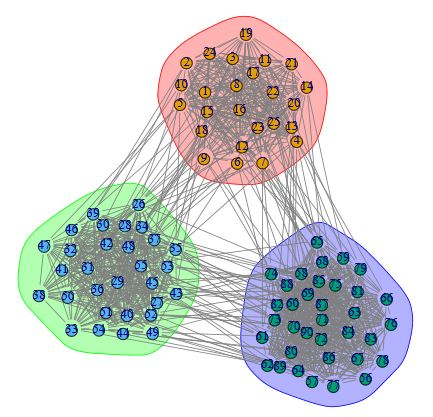
\includegraphics[scale=0.8]{LatexDiss/Dissertation/figs/SBM.JPG}
\caption[Visualization of an SBM-based graph example]{An example of a graph generated using SBM model, the graph has 90 nodes divided into three communities of size 25, 30 and 35 nodes. An edge between two nodes within the same community has a probability 0.8, while it has a probability 0.5 if the two nodes belong to different communities.}
%Source:
\label{fig:SBM_example}
\end{figure}

The basic idea of the standard SBM is that the neighborhood relations of each node only depend on the probabilities assigned to the model. Roughly speaking, the nodes are clustered in a way so that the neighbors of nodes in a group (community) have a similar neighbor pattern as well. To generate a graph $G$ of size $n$ using SBM model, the following parameters should be given: The number of communities (groups) in the graph $L$, node to community assignments ${b_1 , \ldots ,b_n}$ such that node $i$ belongs to community $b_i$, edge probability matrix $(p_{i,j})_{i,j\in\{1,\ldots, L\}}$.
Then the graph is generated by independently add an edge between any two pair of nodes $(u,v)$ with probability $p_{b_u , b_v}$.\newline
An easy thing to compute here is the average degree $d$ of each node $u$ in the graph $G=SBM(V_G, L, b_u, p_{i,j})$, which is equal to:
\begin{equation}
    d_u=\sum_{b\neq b_u} p_{b_u,b}*(\#\{v\in V_G, b_v=b \} )+p_{b_u,b_u}*(\#\{v\in V_G, b_v=b_u \}-1 )
\end{equation}
In our case and almost in every experiment, unless the opposite is mentioned, the dataset consists of 300 graphs constructed by SBM model each, each graph has $n=60$ nodes divided equally between two communities $L=2$. Other parameters ($p_{i,j}$) take different values in different graphs, and actually graphs are divided into different classes based on the corresponding values of these parameters. We consider only the case where the probabilities $p_{1,1}= p_{2,2} = p_{in}$. However,  it is obvious that  $p_{1,2}=p_{2,1}=p_{out}$ since we want an indirect graphs dataset as indicated previously.\newline
The first class of graphs corresponds to a fixed pair ($p_{in,1}, p_{out,1}$) and similarly the second one  corresponds to ($p_{in,2}, p_{out,2}$). These two pairs are always chosen so that any node in any graph in any dataset has an expected average degree equal to 10 (to preserve some difficulty in the classification problem). we refer to $r=(p_{in,1}/p_{in,2})$ by inter-classes similarity parameter, where the closer to one it is the more similar both classes are and thus the harder it is to discriminate them. 

\subsection{Graphlet Kernel results}
\begin{figure}[H]
\centering
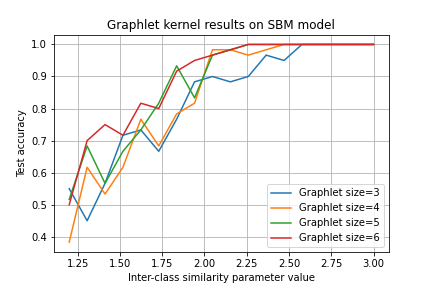
\includegraphics[scale=0.7]{LatexDiss/Dissertation/figs/graphlet_kernel_SBM_accuracy.png}
\caption[Graphlet kernel classification test accuracy as a function of Inter-classes similarity parameter]{Graphlet kernel classification test accuracy with respect to Inter-classes similarity parameter $r$. where per graph G, 2000 graphlet samples are considered to compute its graphlet spectrum vector. }
%Source:
\label{fig:graphlet_kernel_SBM}
\end{figure}

\begin{table}
\begin{center}
\begin{tabular}{|l|c|c|c|c|}
\hline
{}  &  {\sc 3-graphlets}  & {\sc 4-graphlets}  & {\sc 5-graphlets} & {\sc 6-graphlets} \\
\hline
{Computational Time (Sec)}         & 80 & 120 & 150 & 320 \\
\hline
\end{tabular}
\end{center}
\caption{Computational time per epoch of k-graphlet kernel with different k values.}
\label{table:graphlet_time}
\end{table}


\subsection{OPUs' Random Features Results}

\paragraph {Fixed inter-classes similarity and varying number of random features (Fig. \ref{fig:LightOn_adj_SBM_RF})}
\begin{figure}[H]
\centering
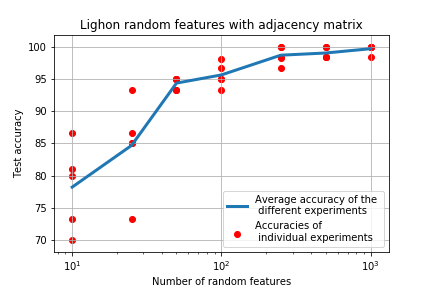
\includegraphics[scale=0.7]{LatexDiss/Dissertation/figs/LightON_adj_SBM_varying_RF.png}
\caption[Classification test accuracy as a function of the number of random features]{Classification test accuracy with respect to the number of LightOn random features. The SVM model is trained on SBM 240-sized labeled dataset. Per graph G, 2000 graphlet samples (Uniform sampling) of size 6 are considered to compute its features map $\phi(G)$. As expected, the accuracy variance drastically decrease as the number of random features increase. }
\label{fig:LightOn_adj_SBM_RF}
\end{figure}
The interesting thing here with OPUs is that the computational time does not really depend on the number of random features  as long as it is within the capacity of the OPU when we consider fixed graphlet size, in this experiment processing time was as specified in Table. \ref{table:OPU_RF_time}. 
\begin{table}[H]
\begin{center}
\begin{tabular}{|l|c|}
\hline
{\sc Computational Time (Sec)}  &  {400 Sec}\\
\hline
\end{tabular}
\end{center}
\caption{Computational time per epoch of OPUs' random features based method.}
\label{table:OPU_RF_time}
\end{table}

\paragraph{Varying inter-classes similarity and fixed number of random features (Fig. \ref{fig:LightOn_adj_SBM_mult_factor})}
The computational time in this case is presented in Table. \ref{table:OPU_multfactor_uniform_time}. We notice that there are slight differences between time values when the graphlet size change, this is due to two reasons, the first one is that OPUs' processing time does not depend on the dimension of the input nor on the number of random features as we respect its capacity, the second one is that we consider Uniform Sampling technique to sub-sample k-size graphlets, which is unlike Random Walk based sampling techniques fast and doesn't require significantly larger time when the graphlet size increases. 
\begin{figure}[H]
\centering
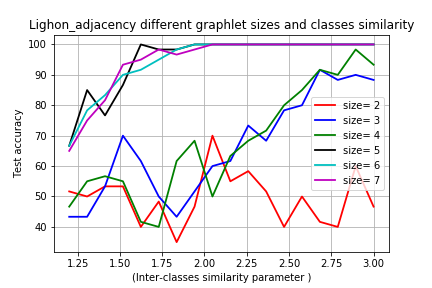
\includegraphics[scale=0.7]{LatexDiss/Dissertation/figs/LightOn_adj_SBM_Similarity_graphlet_size.png}

\caption[Classification test accuracy as a function of Inter-classes similarity parameter ]{Classification test accuracy with respect to Inter-classes similarity parameter when the number of random features is fixed to 5000 but with different sizes of the graphlet to be sampled. The SVM model is trained on SBM 240-sized labeled dataset. Per graph G, 2000 graphlet samples (Uniform sampling) of the corresponding size are considered to compute its features map $\phi(G)$.}
%Source:
\label{fig:LightOn_adj_SBM_mult_factor}
\end{figure}

\begin{table}
\begin{center}
\begin{tabular}{|l|c|c|c|}
\hline
{Graphlet Size}  &  {\sc 3} & {\sc 4}  & {\sc 5} \\
\hline
{Computational Time (Sec)}         & 630 & 720 & 810  \\
\hline
\end{tabular}
\end{center}
\caption{Computational time per epoch of OPUs' random features method using Induced Random walk}
\label{table:OPU_multfactor_IRW_time}
\end{table}


\begin{table}
\begin{center}
\begin{tabular}{|l|c|c|c|c|c|c|}
\hline
{Graphlet Size}  &  {\sc 2} & {\sc 3}  & {\sc 4}  & {\sc 5} & {\sc 6} & {7} \\
\hline
{Computational Time (Sec)}         & 340 & 357 & 362 & 378 & 400 & 412  \\
\hline
\end{tabular}
\end{center}
\caption{Computational time per epoch of OPUs' random features based method using uniform sampling technique.}
\label{table:OPU_multfactor_uniform_time}
\end{table}

\begin{figure}[H]
\centering
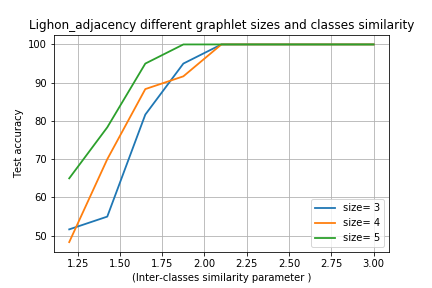
\includegraphics[scale=0.7]{LatexDiss/Dissertation/figs/LightOn_adj_SBM_similarity_graphlet_size_RW.png}
\caption[Classification test accuracy as a function of Inter-classes similarity parameter ]{Classification test accuracy with respect to Inter-classes similarity parameter when the number of random features is fixed to 5000 but with different sizes of the graphlet to be sampled. The SVM model is trained on SBM 240-sized labeled dataset. Per graph G, 2000 graphlet samples (Random Walk sampling) of the corresponding size are considered to compute its features map $\phi(G)$. This experiment is done to check if the uniform sampling technique is the reason behind the gap between accuracy curves of graphlet sizes 4 and 5 in Fig. \ref{fig:LightOn_adj_SBM_mult_factor} }
%Source:
\label{fig:LightOn_adj_SBM_multfactor_RW}
\end{figure}
However, one unexpected thing in Fig. \ref{fig:LightOn_adj_SBM_mult_factor} is that there is notably a gap between 4-graphlet and 5-graphlet curves, to detect the reason behind this gap we ran the same experiment with the same settings but using Induced Random Walk Sampling Technique , which tends to sample nodes that appear in a random walk starting from randomly chosen node (will be further explained in the report later). results are shown in Fig. \ref{fig:LightOn_adj_SBM_multfactor_RW} and the corresponding computational time is shown in Table. \ref{table:OPU_multfactor_IRW_time}.

\paragraph{Graph Convolution Network GCN}
In order to benchmark the results of Random Features-based methods with other common methods used in Graph classification, we modified and trained one of the proposed models built based on GIN (Graph Isomorphism Network), which has been reported to give brilliant results (even better than most of state-of-art classical Graph Convolutional Networks) in classifying graphs based only on their structural information in the absence of node features just like the case of our SBM dataset \citep{GCN_powerful}. 

\begin{figure}[H]
\centering
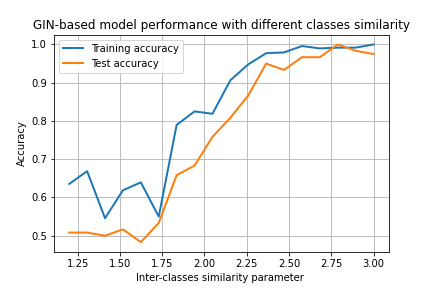
\includegraphics[scale=0.7]{LatexDiss/Dissertation/figs/GNN_GIN.png}

\caption[GCN model's classification test accuracy as a function of Inter-classes similarity parameter ]{GCN model's classification test accuracy with respect to Inter-classes similarity parameter. The  model is trained on SBM 240-sized labeled dataset.}
%Source:
\label{fig:GCN_GIN_SBM_multfactor_RW}
\end{figure}

\begin{table}
\begin{center}
\begin{tabular}{|l|c|c|c|}
\hline
{Epoch processing time (Sec)}  &  {total training time (Sec)} \\
\hline
0.29 & 87  \\
\hline
\end{tabular}
\end{center}
\caption{Computational time per epoch of the GCN GIN-based model.}
\label{table:OPU_multfactor_IRW_time}
\end{table}
The model consists of 5 GIN layers followed by two fully connected layers where the dimensions of hidden layers are equal to 4. Comparing GCN performance to the one we got using OPUs random features (Fig. \ref{fig:LightOn_adj_SBM_multfactor_RW} and Fig. \ref{fig:LightOn_adj_SBM_mult_factor}) we can say that the performance of Random Features based methods is slightly better when the graphlet size is greater than 4, especially using Induced Random Walk sampling technique. However, the training time of GCN model still notably better (I should check if I can do something with LightOn platform to enhance its time, so the report will be fixed later). 

\section{DD Real-world Data set}
\subsection{OPUs’ Random Features Results}
\begin{figure}[H]
\centering
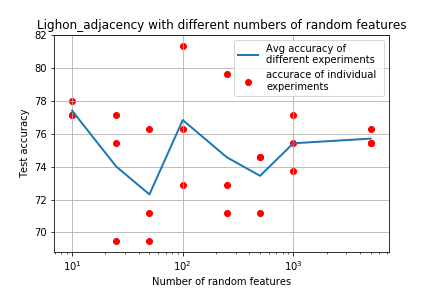
\includegraphics[scale=0.7]{LatexDiss/Dissertation/figs/LightOn_adj_DD_varying_RF.png}

\caption[Classification test accuracy as a function of the number of random features]{Classification test accuracy with respect to the number of random features on DD Dataset}
%Source:
\label{fig:LightON_DD_multfactor_RW}
\end{figure}

%\addchapheadtotoc
\chapter{Results and Discussion}
In this chapter we introduce the experiments conducted in this work  with a discussion of the results. At first, we present the results of a Synthetic Graph Dataset created based on Stochastic Block Model (SBM), then the results of some real-world datasets (DD, Mutag,..etc).


\section{Results of Synthetic SBM Dataset}
\subsection{Stochastic Block Model SBM}
SBM is commonly known in social sciences to model group structures in friendship graph networks. As a combination of the strict block model with a stochastic element, it was able to deal with imperfect group structures and noise of real world networks. The standard SBM does not only determine the likelihood of a specific group structure belonging to a certain network. The model is based on a generative model, which enables the user to generate other network instances from a given structure or allows the prediction of missing edges \citep{SBM}.

\begin{figure}[H]
\centering
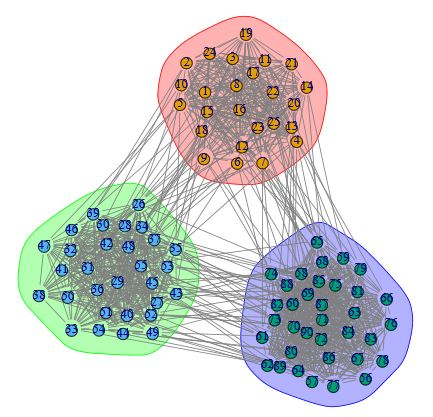
\includegraphics[scale=0.8]{LatexDiss/Dissertation/figs/SBM.JPG}
\caption[Visualization of an SBM-based graph example]{An example of a graph generated using SBM model, the graph has 90 nodes divided into three communities of size 25, 30 and 35 nodes. An edge between two nodes within the same community has a probability 0.8, while it has a probability 0.5 if the two nodes belong to different communities.}
%Source:
\label{fig:SBM_example}
\end{figure}

The basic idea of the standard SBM is that the neighborhood relations of each node only depend on the probabilities assigned to the model. Roughly speaking, the nodes are clustered in a way so that the neighbors of nodes in a group (community) have a similar neighbor pattern as well. To generate a graph $G$ of size $n$ using SBM model, the following parameters should be given: The number of communities (groups) in the graph $L$, node to community assignments ${b_1 , \ldots ,b_n}$ such that node $i$ belongs to community $b_i$, edge probability matrix $(p_{i,j})_{i,j\in\{1,\ldots, L\}}$.
Then the graph is generated by independently add an edge between any two pair of nodes $(u,v)$ with probability $p_{b_u , b_v}$.\newline
An easy thing to compute here is the average degree $d$ of each node $u$ in the graph $G=SBM(V_G, L, b_u, p_{i,j})$, which is equal to:
\begin{equation}
    d_u=\sum_{b\neq b_u} p_{b_u,b}*(\#\{v\in V_G, b_v=b \} )+p_{b_u,b_u}*(\#\{v\in V_G, b_v=b_u \}-1 )
\end{equation}
In our case and almost in every experiment, unless the opposite is mentioned, the dataset consists of 300 graphs constructed by SBM model each, each graph has $n=60$ nodes divided equally between two communities $L=2$. Other parameters ($p_{i,j}$) take different values in different graphs, and actually graphs are divided into different classes based on the corresponding values of these parameters. We consider only the case where the probabilities $p_{1,1}= p_{2,2} = p_{in}$. However,  it is obvious that  $p_{1,2}=p_{2,1}=p_{out}$ since we want an indirect graphs dataset as indicated previously.\newline
The first class of graphs corresponds to a fixed pair ($p_{in,1}, p_{out,1}$) and similarly the second one  corresponds to ($p_{in,2}, p_{out,2}$). These two pairs are always chosen so that any node in any graph in any dataset has an expected average degree equal to 10 (to preserve some difficulty in the classification problem). we refer to $r=(p_{in,1}/p_{in,2})$ by inter-classes similarity parameter, where the closer to one it is the more similar both classes are and thus the harder it is to discriminate them. 

\subsection{Graphlet Kernel results}
\begin{figure}[H]
\centering
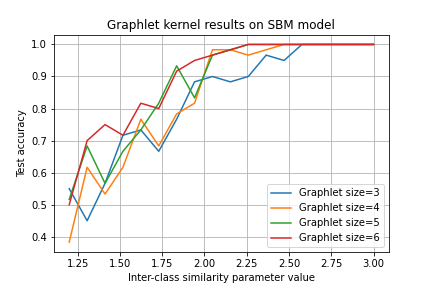
\includegraphics[scale=0.7]{LatexDiss/Dissertation/figs/graphlet_kernel_SBM_accuracy.png}
\caption[Graphlet kernel classification test accuracy as a function of Inter-classes similarity parameter]{Graphlet kernel classification test accuracy with respect to Inter-classes similarity parameter $r$. where per graph G, 2000 graphlet samples are considered to compute its graphlet spectrum vector. }
%Source:
\label{fig:graphlet_kernel_SBM}
\end{figure}

\begin{table}
\begin{center}
\begin{tabular}{|l|c|c|c|c|}
\hline
{}  &  {\sc 3-graphlets}  & {\sc 4-graphlets}  & {\sc 5-graphlets} & {\sc 6-graphlets} \\
\hline
{Computational Time (Sec)}         & 80 & 120 & 150 & 320 \\
\hline
\end{tabular}
\end{center}
\caption{Computational time per epoch of k-graphlet kernel with different k values.}
\label{table:graphlet_time}
\end{table}


\subsection{OPUs' Random Features Results}

\paragraph {Fixed inter-classes similarity and varying number of random features (Fig. \ref{fig:LightOn_adj_SBM_RF})}
\begin{figure}[H]
\centering
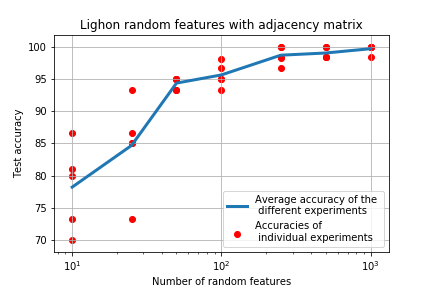
\includegraphics[scale=0.7]{LatexDiss/Dissertation/figs/LightON_adj_SBM_varying_RF.png}
\caption[Classification test accuracy as a function of the number of random features]{Classification test accuracy with respect to the number of LightOn random features. The SVM model is trained on SBM 240-sized labeled dataset. Per graph G, 2000 graphlet samples (Uniform sampling) of size 6 are considered to compute its features map $\phi(G)$. As expected, the accuracy variance drastically decrease as the number of random features increase. }
\label{fig:LightOn_adj_SBM_RF}
\end{figure}
The interesting thing here with OPUs is that the computational time does not really depend on the number of random features  as long as it is within the capacity of the OPU when we consider fixed graphlet size, in this experiment processing time was as specified in Table. \ref{table:OPU_RF_time}. 
\begin{table}[H]
\begin{center}
\begin{tabular}{|l|c|}
\hline
{\sc Computational Time (Sec)}  &  {400 Sec}\\
\hline
\end{tabular}
\end{center}
\caption{Computational time per epoch of OPUs' random features based method.}
\label{table:OPU_RF_time}
\end{table}

\paragraph{Varying inter-classes similarity and fixed number of random features (Fig. \ref{fig:LightOn_adj_SBM_mult_factor})}
The computational time in this case is presented in Table. \ref{table:OPU_multfactor_uniform_time}. We notice that there are slight differences between time values when the graphlet size change, this is due to two reasons, the first one is that OPUs' processing time does not depend on the dimension of the input nor on the number of random features as we respect its capacity, the second one is that we consider Uniform Sampling technique to sub-sample k-size graphlets, which is unlike Random Walk based sampling techniques fast and doesn't require significantly larger time when the graphlet size increases. 
\begin{figure}[H]
\centering
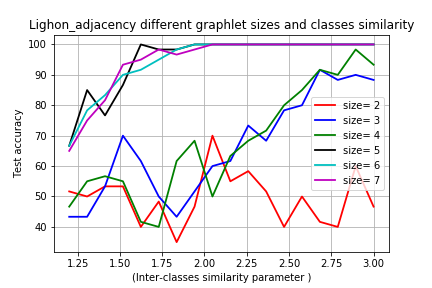
\includegraphics[scale=0.7]{LatexDiss/Dissertation/figs/LightOn_adj_SBM_Similarity_graphlet_size.png}

\caption[Classification test accuracy as a function of Inter-classes similarity parameter ]{Classification test accuracy with respect to Inter-classes similarity parameter when the number of random features is fixed to 5000 but with different sizes of the graphlet to be sampled. The SVM model is trained on SBM 240-sized labeled dataset. Per graph G, 2000 graphlet samples (Uniform sampling) of the corresponding size are considered to compute its features map $\phi(G)$.}
%Source:
\label{fig:LightOn_adj_SBM_mult_factor}
\end{figure}

\begin{table}
\begin{center}
\begin{tabular}{|l|c|c|c|}
\hline
{Graphlet Size}  &  {\sc 3} & {\sc 4}  & {\sc 5} \\
\hline
{Computational Time (Sec)}         & 630 & 720 & 810  \\
\hline
\end{tabular}
\end{center}
\caption{Computational time per epoch of OPUs' random features method using Induced Random walk}
\label{table:OPU_multfactor_IRW_time}
\end{table}


\begin{table}
\begin{center}
\begin{tabular}{|l|c|c|c|c|c|c|}
\hline
{Graphlet Size}  &  {\sc 2} & {\sc 3}  & {\sc 4}  & {\sc 5} & {\sc 6} & {7} \\
\hline
{Computational Time (Sec)}         & 340 & 357 & 362 & 378 & 400 & 412  \\
\hline
\end{tabular}
\end{center}
\caption{Computational time per epoch of OPUs' random features based method using uniform sampling technique.}
\label{table:OPU_multfactor_uniform_time}
\end{table}

\begin{figure}[H]
\centering
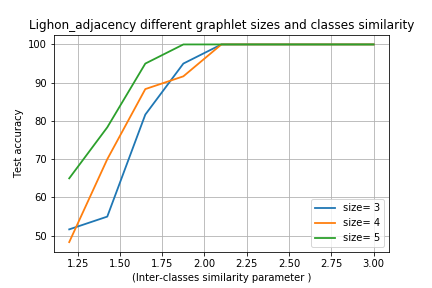
\includegraphics[scale=0.7]{LatexDiss/Dissertation/figs/LightOn_adj_SBM_similarity_graphlet_size_RW.png}
\caption[Classification test accuracy as a function of Inter-classes similarity parameter ]{Classification test accuracy with respect to Inter-classes similarity parameter when the number of random features is fixed to 5000 but with different sizes of the graphlet to be sampled. The SVM model is trained on SBM 240-sized labeled dataset. Per graph G, 2000 graphlet samples (Random Walk sampling) of the corresponding size are considered to compute its features map $\phi(G)$. This experiment is done to check if the uniform sampling technique is the reason behind the gap between accuracy curves of graphlet sizes 4 and 5 in Fig. \ref{fig:LightOn_adj_SBM_mult_factor} }
%Source:
\label{fig:LightOn_adj_SBM_multfactor_RW}
\end{figure}
However, one unexpected thing in Fig. \ref{fig:LightOn_adj_SBM_mult_factor} is that there is notably a gap between 4-graphlet and 5-graphlet curves, to detect the reason behind this gap we ran the same experiment with the same settings but using Induced Random Walk Sampling Technique , which tends to sample nodes that appear in a random walk starting from randomly chosen node (will be further explained in the report later). results are shown in Fig. \ref{fig:LightOn_adj_SBM_multfactor_RW} and the corresponding computational time is shown in Table. \ref{table:OPU_multfactor_IRW_time}.
\paragraph{Varying number of graphlet samples and fixing other parameters }
.

..

.
\subsection{Graph Convolution Network GCN}
In order to benchmark the results of Random Features-based methods with other common methods used in Graph classification, we modified and trained one of the proposed models built based on GIN (Graph Isomorphism Network), which has been reported to give brilliant results (even better than most of state-of-art classical Graph Convolutional Networks) in classifying graphs based only on their structural information in the absence of node features just like the case of our SBM dataset \citep{GCN_powerful}. 

\begin{figure}[H]
\centering
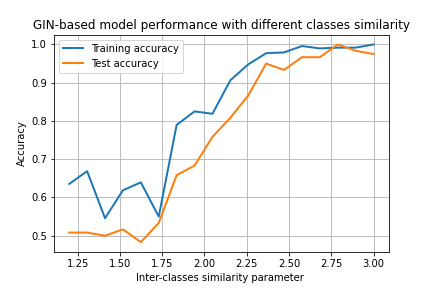
\includegraphics[scale=0.7]{LatexDiss/Dissertation/figs/GNN_GIN.png}

\caption[GCN model's classification test accuracy as a function of Inter-classes similarity parameter ]{GCN model's classification test accuracy with respect to Inter-classes similarity parameter. The  model is trained on SBM 240-sized labeled dataset.}
%Source:
\label{fig:GCN_GIN_SBM_multfactor_RW}
\end{figure}

\begin{table}
\begin{center}
\begin{tabular}{|l|c|c|c|}
\hline
{Epoch processing time (Sec)}  &  {total training time (Sec)} \\
\hline
0.29 & 87  \\
\hline
\end{tabular}
\end{center}
\caption{Computational time per epoch of the GCN GIN-based model.}
\label{table:OPU_multfactor_IRW_time}
\end{table}
The model consists of 5 GIN layers followed by two fully connected layers where the dimensions of hidden layers are equal to 4. Comparing GCN performance to the one we got using OPUs random features (Fig. \ref{fig:LightOn_adj_SBM_multfactor_RW} and Fig. \ref{fig:LightOn_adj_SBM_mult_factor}) we can say that the performance of Random Features based methods is slightly better when the graphlet size is greater than 4, especially using Induced Random Walk sampling technique. However, the training time of GCN model still notably better (I should check if I can do something with LightOn platform to enhance its time, so the report will be fixed later). 

\section{DD Real-world Data set}
\subsection{Graphlet Kernel Results}
.

.

.
\subsection{OPUs’ Random Features Results}
\begin{figure}[H]
\centering
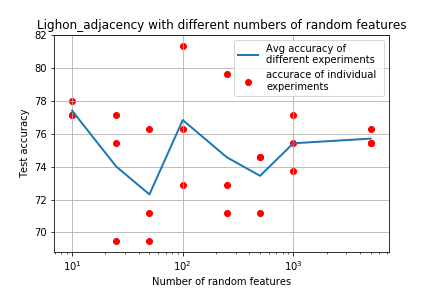
\includegraphics[scale=0.7]{LatexDiss/Dissertation/figs/LightOn_adj_DD_varying_RF.png}

\caption[Classification test accuracy as a function of the number of random features]{Classification test accuracy with respect to the number of random features on DD Dataset}
%Source:
\label{fig:LightON_DD_multfactor_RW}
\end{figure}

\subsection{Graph Convolutional Networks GCNs Results}
.

.

.
%

\chapter{MATHEMATICS NOTATION}
\section{Some Math Stuff}
LaTeX{} has a special way to embed mathematical symbols and notations. Here are some of them. Also observe how a bullet list is made.
\begin{itemize}\itemsep0pt \parskip0pt \parsep0pt
\item greater than $\ge$
\item less than $\le$
\item percent sign \%
\item multiply $N\times N$
\item inline equation $M = N(N-1)/2$
\end{itemize}
Sed orci justo, rutrum in dolor a, consequat dictum mi. Sed luctus congue ex nec dignissim. Phasellus volutpat urna vestibulum ipsum vestibulum, quis venenatis justo consectetur. Nullam hendrerit nisl in rutrum convallis. Sed sit amet malesuada nisi. Phasellus dolor neque, vehicula vestibulum semper at, facilisis eget libero. Mauris interdum magna molestie, auctor felis a, condimentum odio. Pellentesque habitant morbi tristique senectus et netus et malesuada fames ac turpis egestas. Suspendisse maximus lacinia dignissim. Maecenas pharetra accumsan metus, sagittis dictum purus sollicitudin eget. Curabitur ut porttitor arcu, ut porttitor ipsum. Vestibulum porttitor finibus sapien, ac pharetra odio bibendum nec. Nullam tincidunt dignissim risus imperdiet dictum.

Pellentesque habitant morbi tristique senectus et netus et malesuada fames ac turpis egestas. Suspendisse maximus lacinia dignissim. Maecenas pharetra accumsan metus, sagittis dictum purus sollicitudin eget. Curabitur ut porttitor arcu, ut porttitor ipsum. Vestibulum porttitor finibus sapien, ac pharetra odio bibendum nec. Nullam tincidunt dignissim risus imperdiet dictum.
\section{Math equation}
Example of a mathematical formula:
\begin{equation}
  ADD = \sum_{i=1}^{M}|<D(n+1,i)>-<D(n,i)>|
  \label{add}
\end{equation}

Pellentesque habitant morbi tristique senectus et netus et malesuada fames ac turpis egestas. Suspendisse maximus lacinia dignissim. Maecenas pharetra accumsan metus, sagittis dictum purus sollicitudin eget. Curabitur ut porttitor arcu, ut porttitor ipsum. Vestibulum porttitor finibus sapien, ac pharetra odio bibendum nec. Nullam tincidunt dignissim risus imperdiet dictum.
\section{Chapter section}
Fusce ultricies pulvinar diam sed ultrices. Sed orci justo, rutrum in dolor a, consequat dictum mi. Sed luctus congue ex nec dignissim. Phasellus volutpat urna vestibulum ipsum vestibulum, quis venenatis justo consectetur. Nullam hendrerit nisl in rutrum convallis. Sed sit amet malesuada nisi. Phasellus dolor neque, vehicula vestibulum semper at, facilisis eget libero. Mauris interdum magna molestie, auctor felis a, condimentum odio. Pellentesque habitant morbi tristique senectus et netus et malesuada fames ac turpis egestas. Suspendisse maximus lacinia dignissim. Maecenas pharetra accumsan metus, sagittis dictum purus sollicitudin eget. Curabitur ut porttitor arcu, ut porttitor ipsum. Vestibulum porttitor finibus sapien, ac pharetra odio bibendum nec. Nullam tincidunt dignissim risus imperdiet dictum.

Pellentesque habitant morbi tristique senectus et netus et malesuada fames ac turpis egestas. Suspendisse maximus lacinia dignissim. Maecenas pharetra accumsan metus, sagittis dictum purus sollicitudin eget. Curabitur ut porttitor arcu, ut porttitor ipsum. Vestibulum porttitor finibus sapien, ac pharetra odio bibendum nec. Nullam tincidunt dignissim risus imperdiet dictum.

\section{Chapter section}
Fusce ultricies pulvinar diam sed ultrices. Sed orci justo, rutrum in dolor a, consequat dictum mi. Sed luctus congue ex nec dignissim. Phasellus volutpat urna vestibulum ipsum vestibulum, quis venenatis justo consectetur. Nullam hendrerit nisl in rutrum convallis. Sed sit amet malesuada nisi. Phasellus dolor neque, vehicula vestibulum semper at, facilisis eget libero. Mauris interdum magna molestie, auctor felis a, condimentum odio. Pellentesque habitant morbi tristique senectus et netus et malesuada fames ac turpis egestas. Suspendisse maximus lacinia dignissim. Maecenas pharetra accumsan metus, sagittis dictum purus sollicitudin eget. Curabitur ut porttitor arcu, ut porttitor ipsum. Vestibulum porttitor finibus sapien, ac pharetra odio bibendum nec. Nullam tincidunt dignissim risus imperdiet dictum.

Pellentesque habitant morbi tristique senectus et netus et malesuada fames ac turpis egestas. Suspendisse maximus lacinia dignissim. Maecenas pharetra accumsan metus, sagittis dictum purus sollicitudin eget. Curabitur ut porttitor arcu, ut porttitor ipsum. Vestibulum porttitor finibus sapien, ac pharetra odio bibendum nec. Nullam tincidunt dignissim risus imperdiet dictum.

\chapter{FIGURES AND TABLES}
\section{Examples of a figure}
Fusce ultricies pulvinar diam sed ultrices. Sed orci justo, rutrum in dolor a, consequat dictum mi. Sed luctus congue ex nec dignissim. Phasellus volutpat urna vestibulum ipsum vestibulum, quis venenatis justo consectetur. Nullam hendrerit nisl in rutrum convallis. Sed sit amet malesuada nisi.

Example of a figure.
\begin{figure}[ht!]
\begin{center}
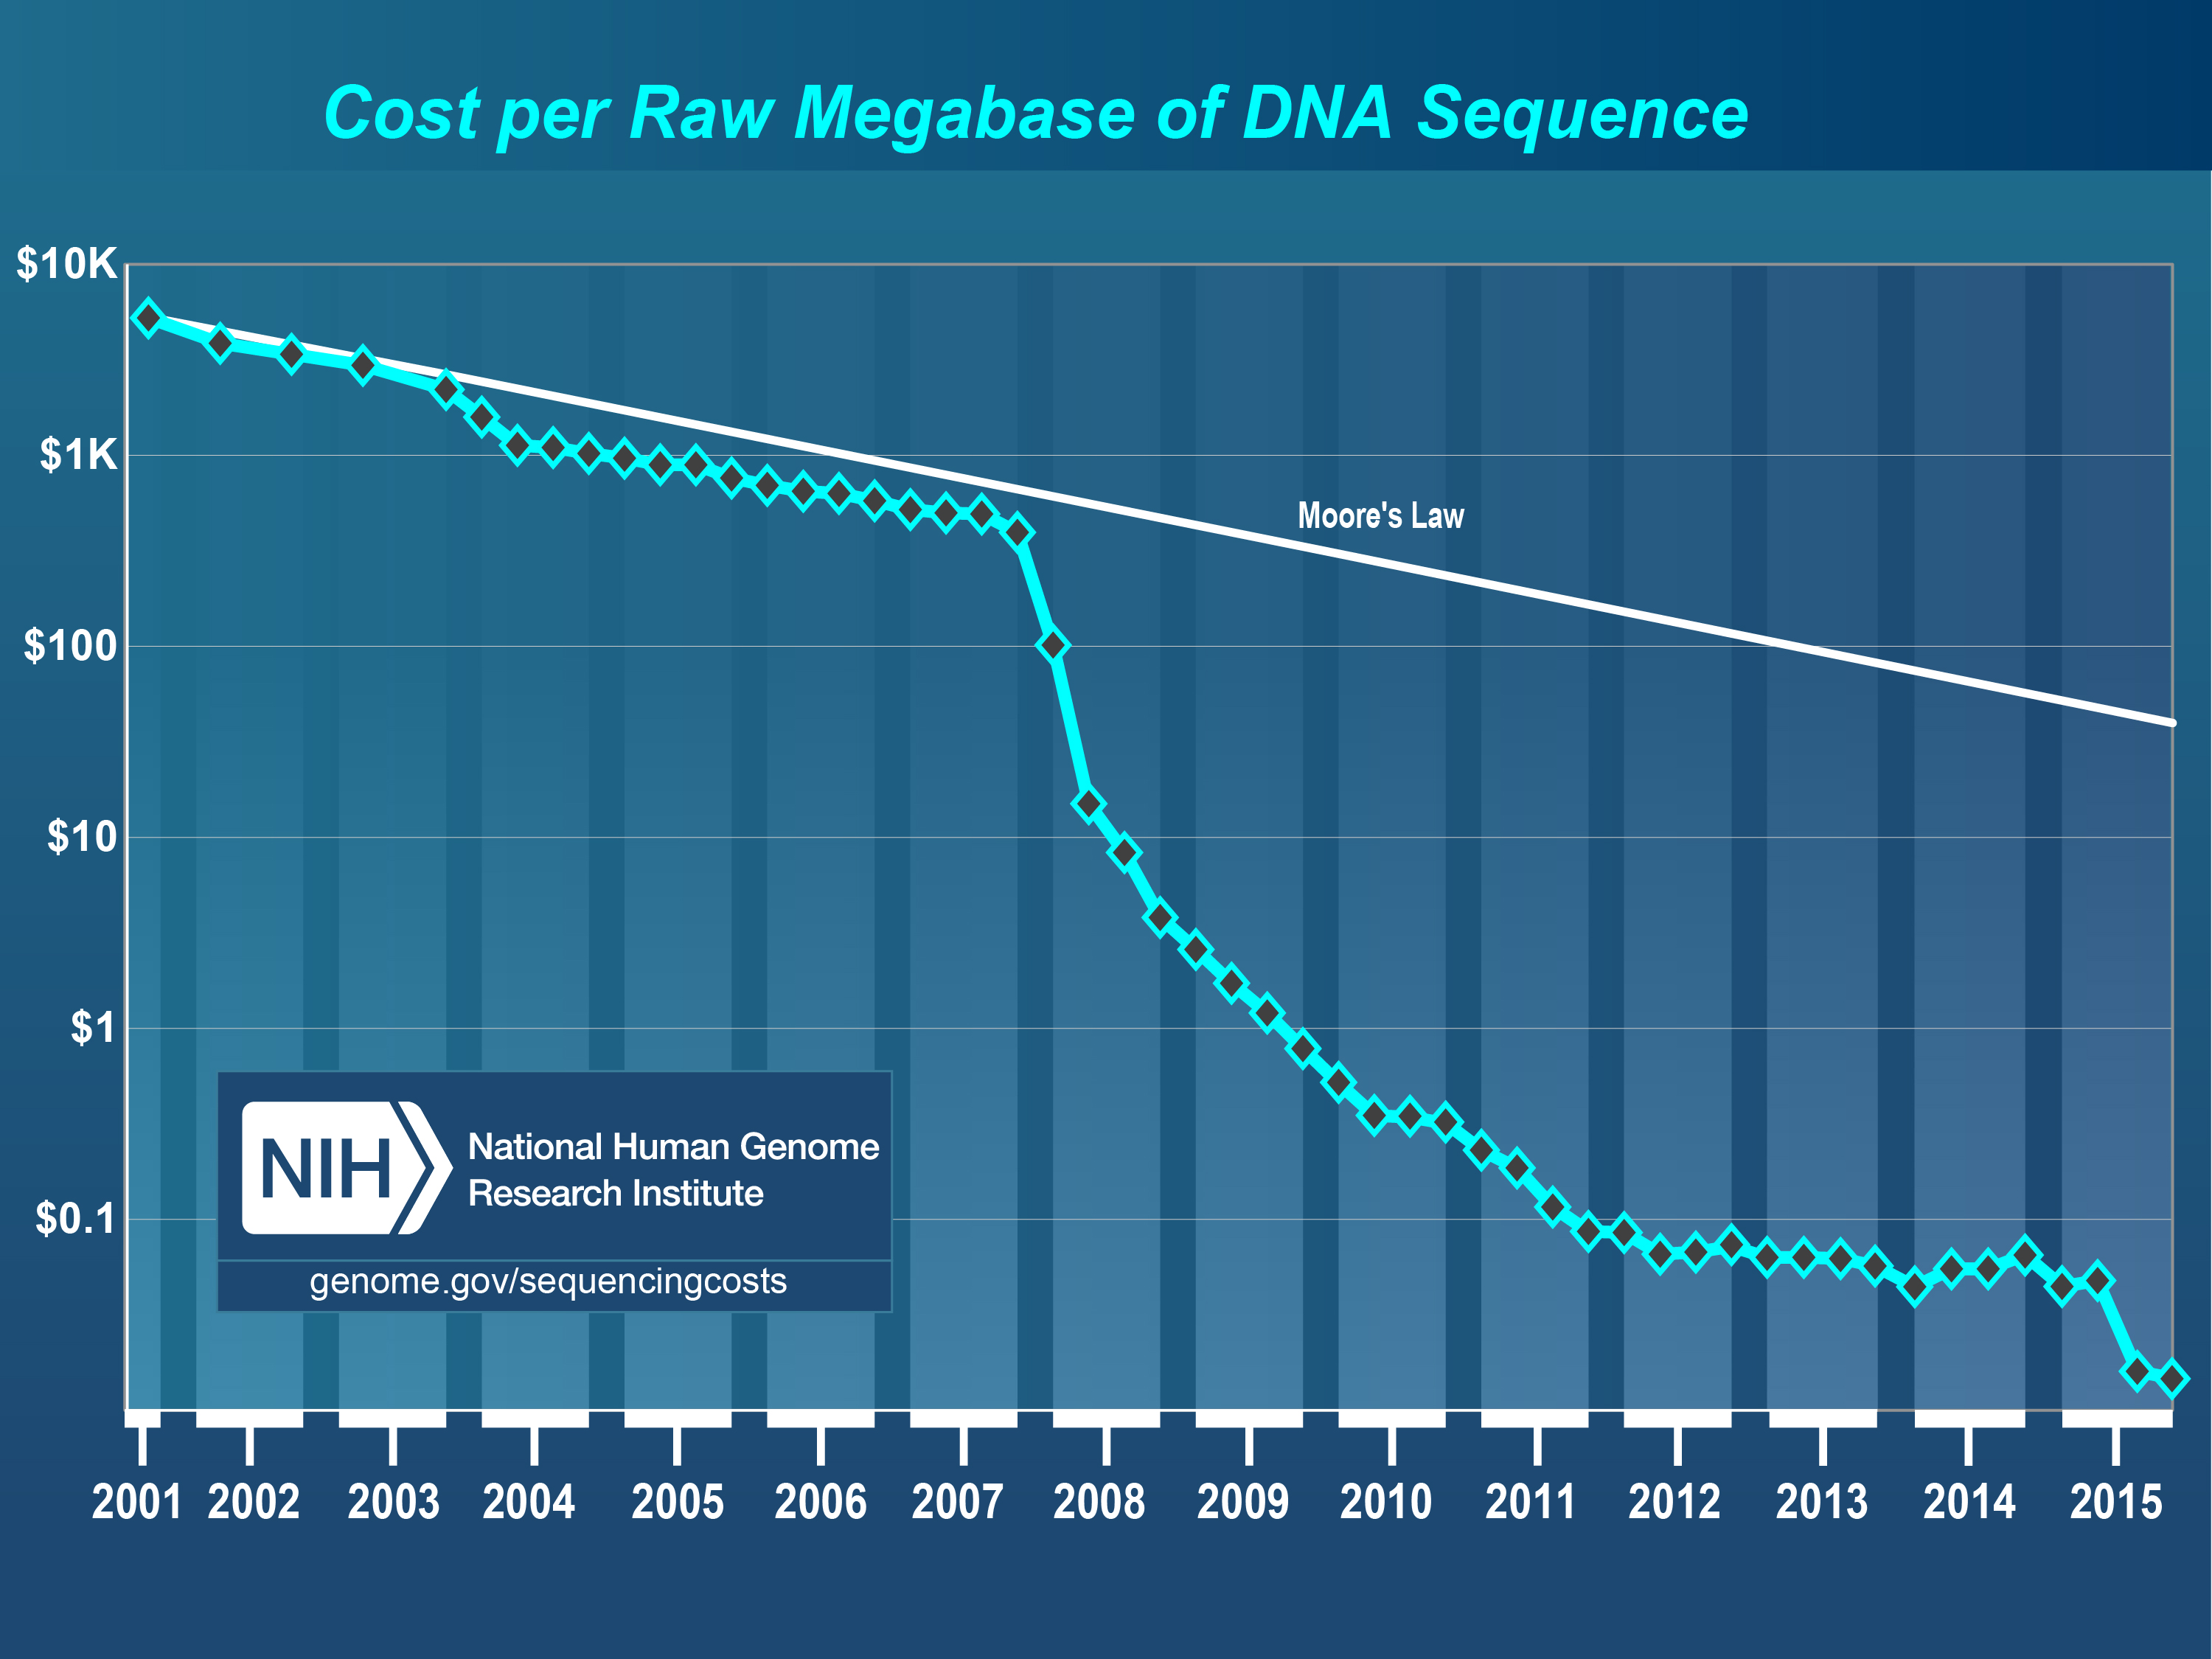
\includegraphics[scale=0.5]{costperMb2015_4.jpg}
\end{center}
\caption[Cost per raw megabase of DNA sequence from 2001 to 2015]{Cost per raw megabase of DNA sequence from 2001 to 2015. Straight line - Moore's Law, blue curve - cost in US dollars, Y-axis scale is logarithmic. Graph reproduced from \citep{wetterstrand2016}}
%Source:
\label{fig_dna_cost}
\end{figure}
Example of reference to a figure in the text (Fig.~\ref{fig_dna_cost}). Phasellus dolor neque, vehicula vestibulum semper at, facilisis eget libero. Mauris interdum magna molestie, auctor felis a, condimentum odio. Pellentesque habitant morbi tristique senectus et netus et malesuada fames ac turpis egestas. Suspendisse maximus lacinia dignissim. Maecenas pharetra accumsan metus, sagittis dictum purus sollicitudin eget. Curabitur ut porttitor arcu, ut porttitor ipsum. Vestibulum porttitor finibus sapien, ac pharetra odio bibendum nec. Nullam tincidunt dignissim risus imperdiet dictum.

Pellentesque habitant morbi tristique senectus et netus et malesuada fames ac turpis egestas. Suspendisse maximus lacinia dignissim. Maecenas pharetra accumsan metus, sagittis dictum purus sollicitudin eget. Curabitur ut porttitor arcu, ut porttitor ipsum. Vestibulum porttitor finibus sapien, ac pharetra odio bibendum nec. Nullam tincidunt dignissim risus imperdiet dictum.
\section{Example of a table}
Example of a table and here is the reference to Table \ref{table_genomes}. Tables in, my opinion, are the hardest thing to make.

\begin{table}
\begin{center}
\begin{tabular}{|l|c|c|c|}
\hline
{\sc Organism}  &  {\sc Accession no.}  & {\sc Genome size} (bp)  & {\sc No. CDS} \\
\hline
{\it Mesorhizobium loti}          & NC\_002678 & 7036071 & 6743 \\
\hline
{\it Sinorhizobium meliloti}      & NC\_003047 & 3654135 & 3359 \\
\hline
{\it Bradyrhizobium japonicum}    & NC\_004463 & 9105828 & 8317 \\
\hline
{\it Rhodopseudomonas palustris}  & NC\_005296 & 5459213 & 4813 \\
\hline
{\it Bartonella quintana}         & NC\_005955 & 1581384 & 1142 \\
\hline
{\it Bartonella henselae}         & NC\_005956 & 1931047 & 1488 \\
\hline
{\it Rickettsia typhi}            & NC\_006142 & 1111496 & 837 \\
\hline
{\it Beijerinckia indica}         & NC\_010581 & 4170153 & 3569 \\
\hline
\end{tabular}
\end{center}
\caption{Whole-genome sequences used in this study}
\label{table_genomes}
\end{table}

Fusce ultricies pulvinar diam sed ultrices. Sed orci justo, rutrum in dolor a, consequat dictum mi. Sed luctus congue ex nec dignissim. Phasellus volutpat urna vestibulum ipsum vestibulum, quis venenatis justo consectetur. Nullam hendrerit nisl in rutrum convallis. Sed sit amet malesuada nisi. Phasellus dolor neque, vehicula vestibulum semper at, facilisis eget libero. Mauris interdum magna molestie, auctor felis a, condimentum odio. Pellentesque habitant morbi tristique senectus et netus et malesuada fames ac turpis egestas. Suspendisse maximus lacinia dignissim. Maecenas pharetra accumsan metus, sagittis dictum purus sollicitudin eget. Curabitur ut porttitor arcu, ut porttitor ipsum. Vestibulum porttitor finibus sapien, ac pharetra odio bibendum nec. Nullam tincidunt dignissim risus imperdiet dictum.

Pellentesque habitant morbi tristique senectus et netus et malesuada fames ac turpis egestas. Suspendisse maximus lacinia dignissim. Maecenas pharetra accumsan metus, sagittis dictum purus sollicitudin eget. Curabitur ut porttitor arcu, ut porttitor ipsum. Vestibulum porttitor finibus sapien, ac pharetra odio bibendum nec. Nullam tincidunt dignissim risus imperdiet dictum.
\section{Chapter section}
Fusce ultricies pulvinar diam sed ultrices. Sed orci justo, rutrum in dolor a, consequat dictum mi. Sed luctus congue ex nec dignissim. Phasellus volutpat urna vestibulum ipsum vestibulum, quis venenatis justo consectetur. Nullam hendrerit nisl in rutrum convallis. Sed sit amet malesuada nisi. Phasellus dolor neque, vehicula vestibulum semper at, facilisis eget libero. Mauris interdum magna molestie, auctor felis a, condimentum odio. Pellentesque habitant morbi tristique senectus et netus et malesuada fames ac turpis egestas. Suspendisse maximus lacinia dignissim. Maecenas pharetra accumsan metus, sagittis dictum purus sollicitudin eget. Curabitur ut porttitor arcu, ut porttitor ipsum. Vestibulum porttitor finibus sapien, ac pharetra odio bibendum nec. Nullam tincidunt dignissim risus imperdiet dictum.

Pellentesque habitant morbi tristique senectus et netus et malesuada fames ac turpis egestas. Suspendisse maximus lacinia dignissim. Maecenas pharetra accumsan metus, sagittis dictum purus sollicitudin eget. Curabitur ut porttitor arcu, ut porttitor ipsum. Vestibulum porttitor finibus sapien, ac pharetra odio bibendum nec. Nullam tincidunt dignissim risus imperdiet dictum.


% Bibliography
\begingroup
    \setlength\bibitemsep{10pt}
    \linespread{1}\selectfont
    \printbibliography[title=REFERENCES]
\endgroup
\addcontentsline{toc}{part}{REFERENCES}

% Appendices
%\appendix

%%%%%%%%%% DON'T DELETE THIS, REVERTS NUMBERING BACK %%%%%%%%%%%%%
\makeatletter
\renewcommand{\@makechapterhead}[1]{\vspace *{-10\p@ }{\parindent \z@ 
\raggedright \normalfont \ifnum \c@secnumdepth >\m@ne \Huge \bfseries 
\@chapapp \space \thechapter \vskip 10\p@ \fi #1\par \nobreak \vskip 30\p@ }}
\makeatother
%%%%%%%%%% DON'T DELETE THIS, REVERTS NUMBERING BACK %%%%%%%%%%%%%

\chapter{}
\vspace*{-0.3in}
\begin{figure}[hb!]
\begin{center}
\makebox[\textwidth][c]{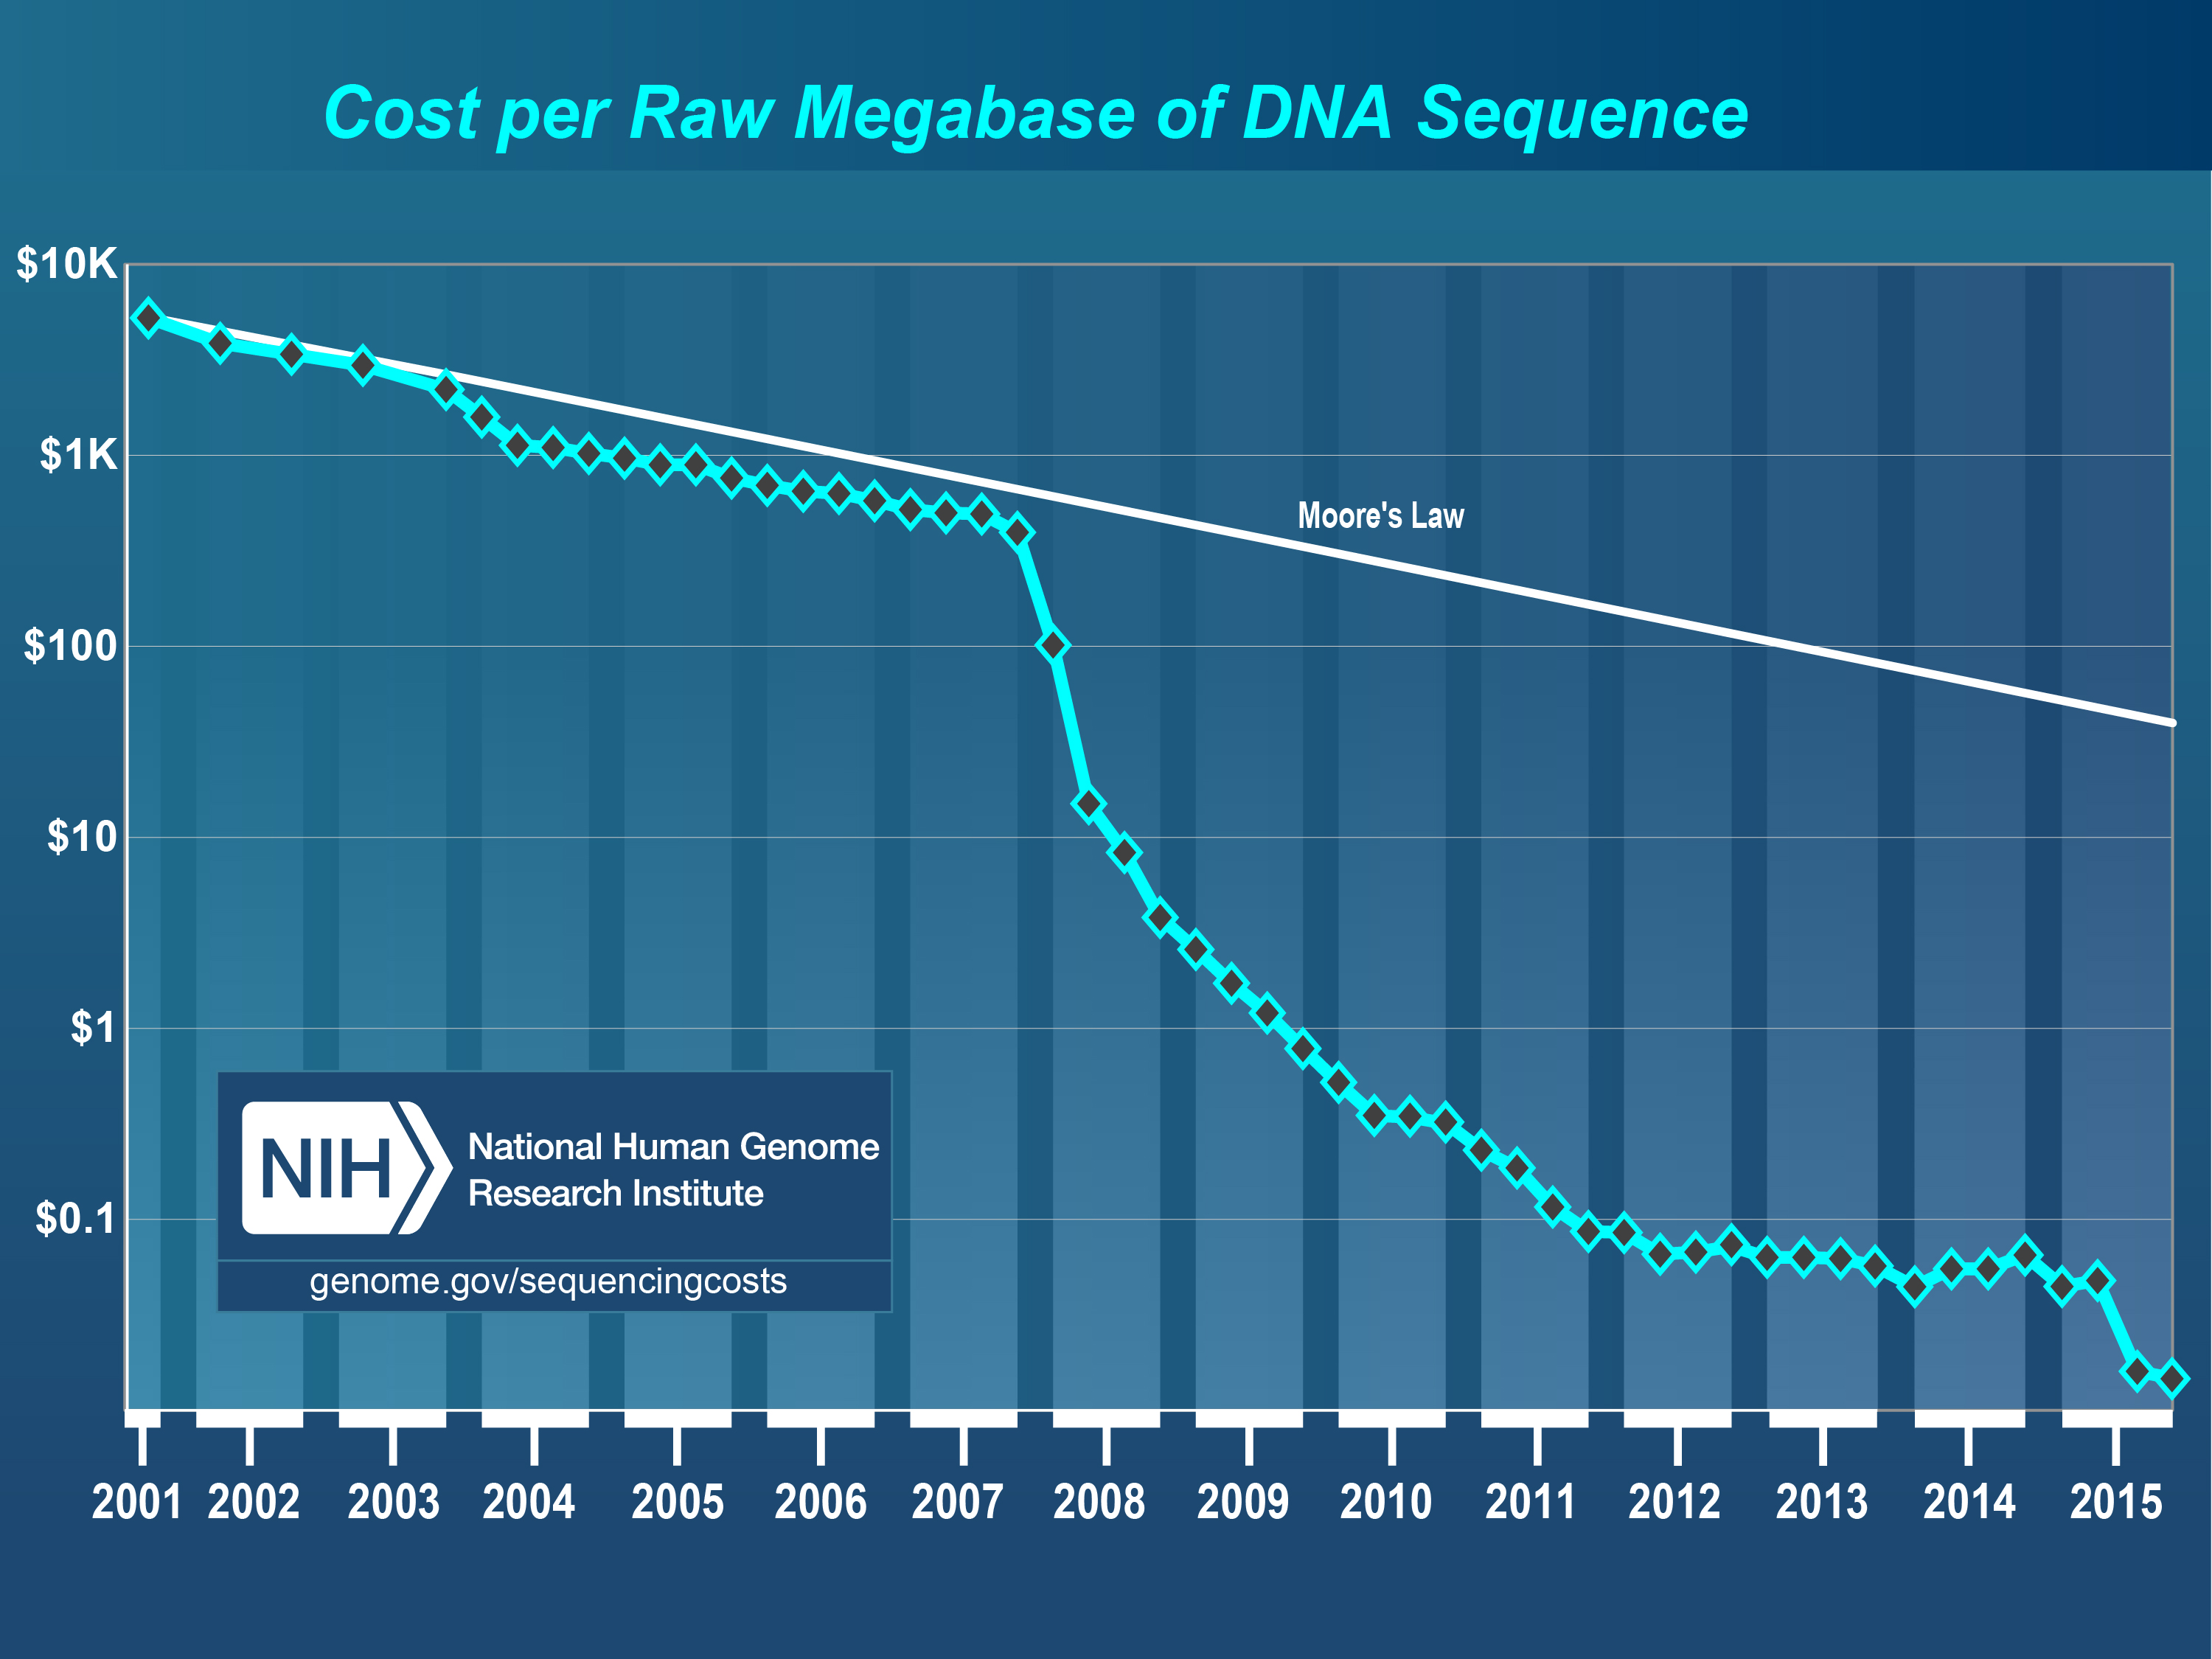
\includegraphics[width=1.0\textwidth]{costperMb2015_4.jpg}}
\end{center}
\caption[Cost per raw megabase of DNA sequence from 2001 to 2015]{Cost per raw megabase of DNA sequence from 2001 to 2015. Straight line - Moore's Law, blue curve - cost in US dollars, Y-axis scale is logarithmic. Graph reproduced from \citep{wetterstrand2016}}
\end{figure}
\begin{figure}[hb!]
\begin{center}
\makebox[\textwidth][c]{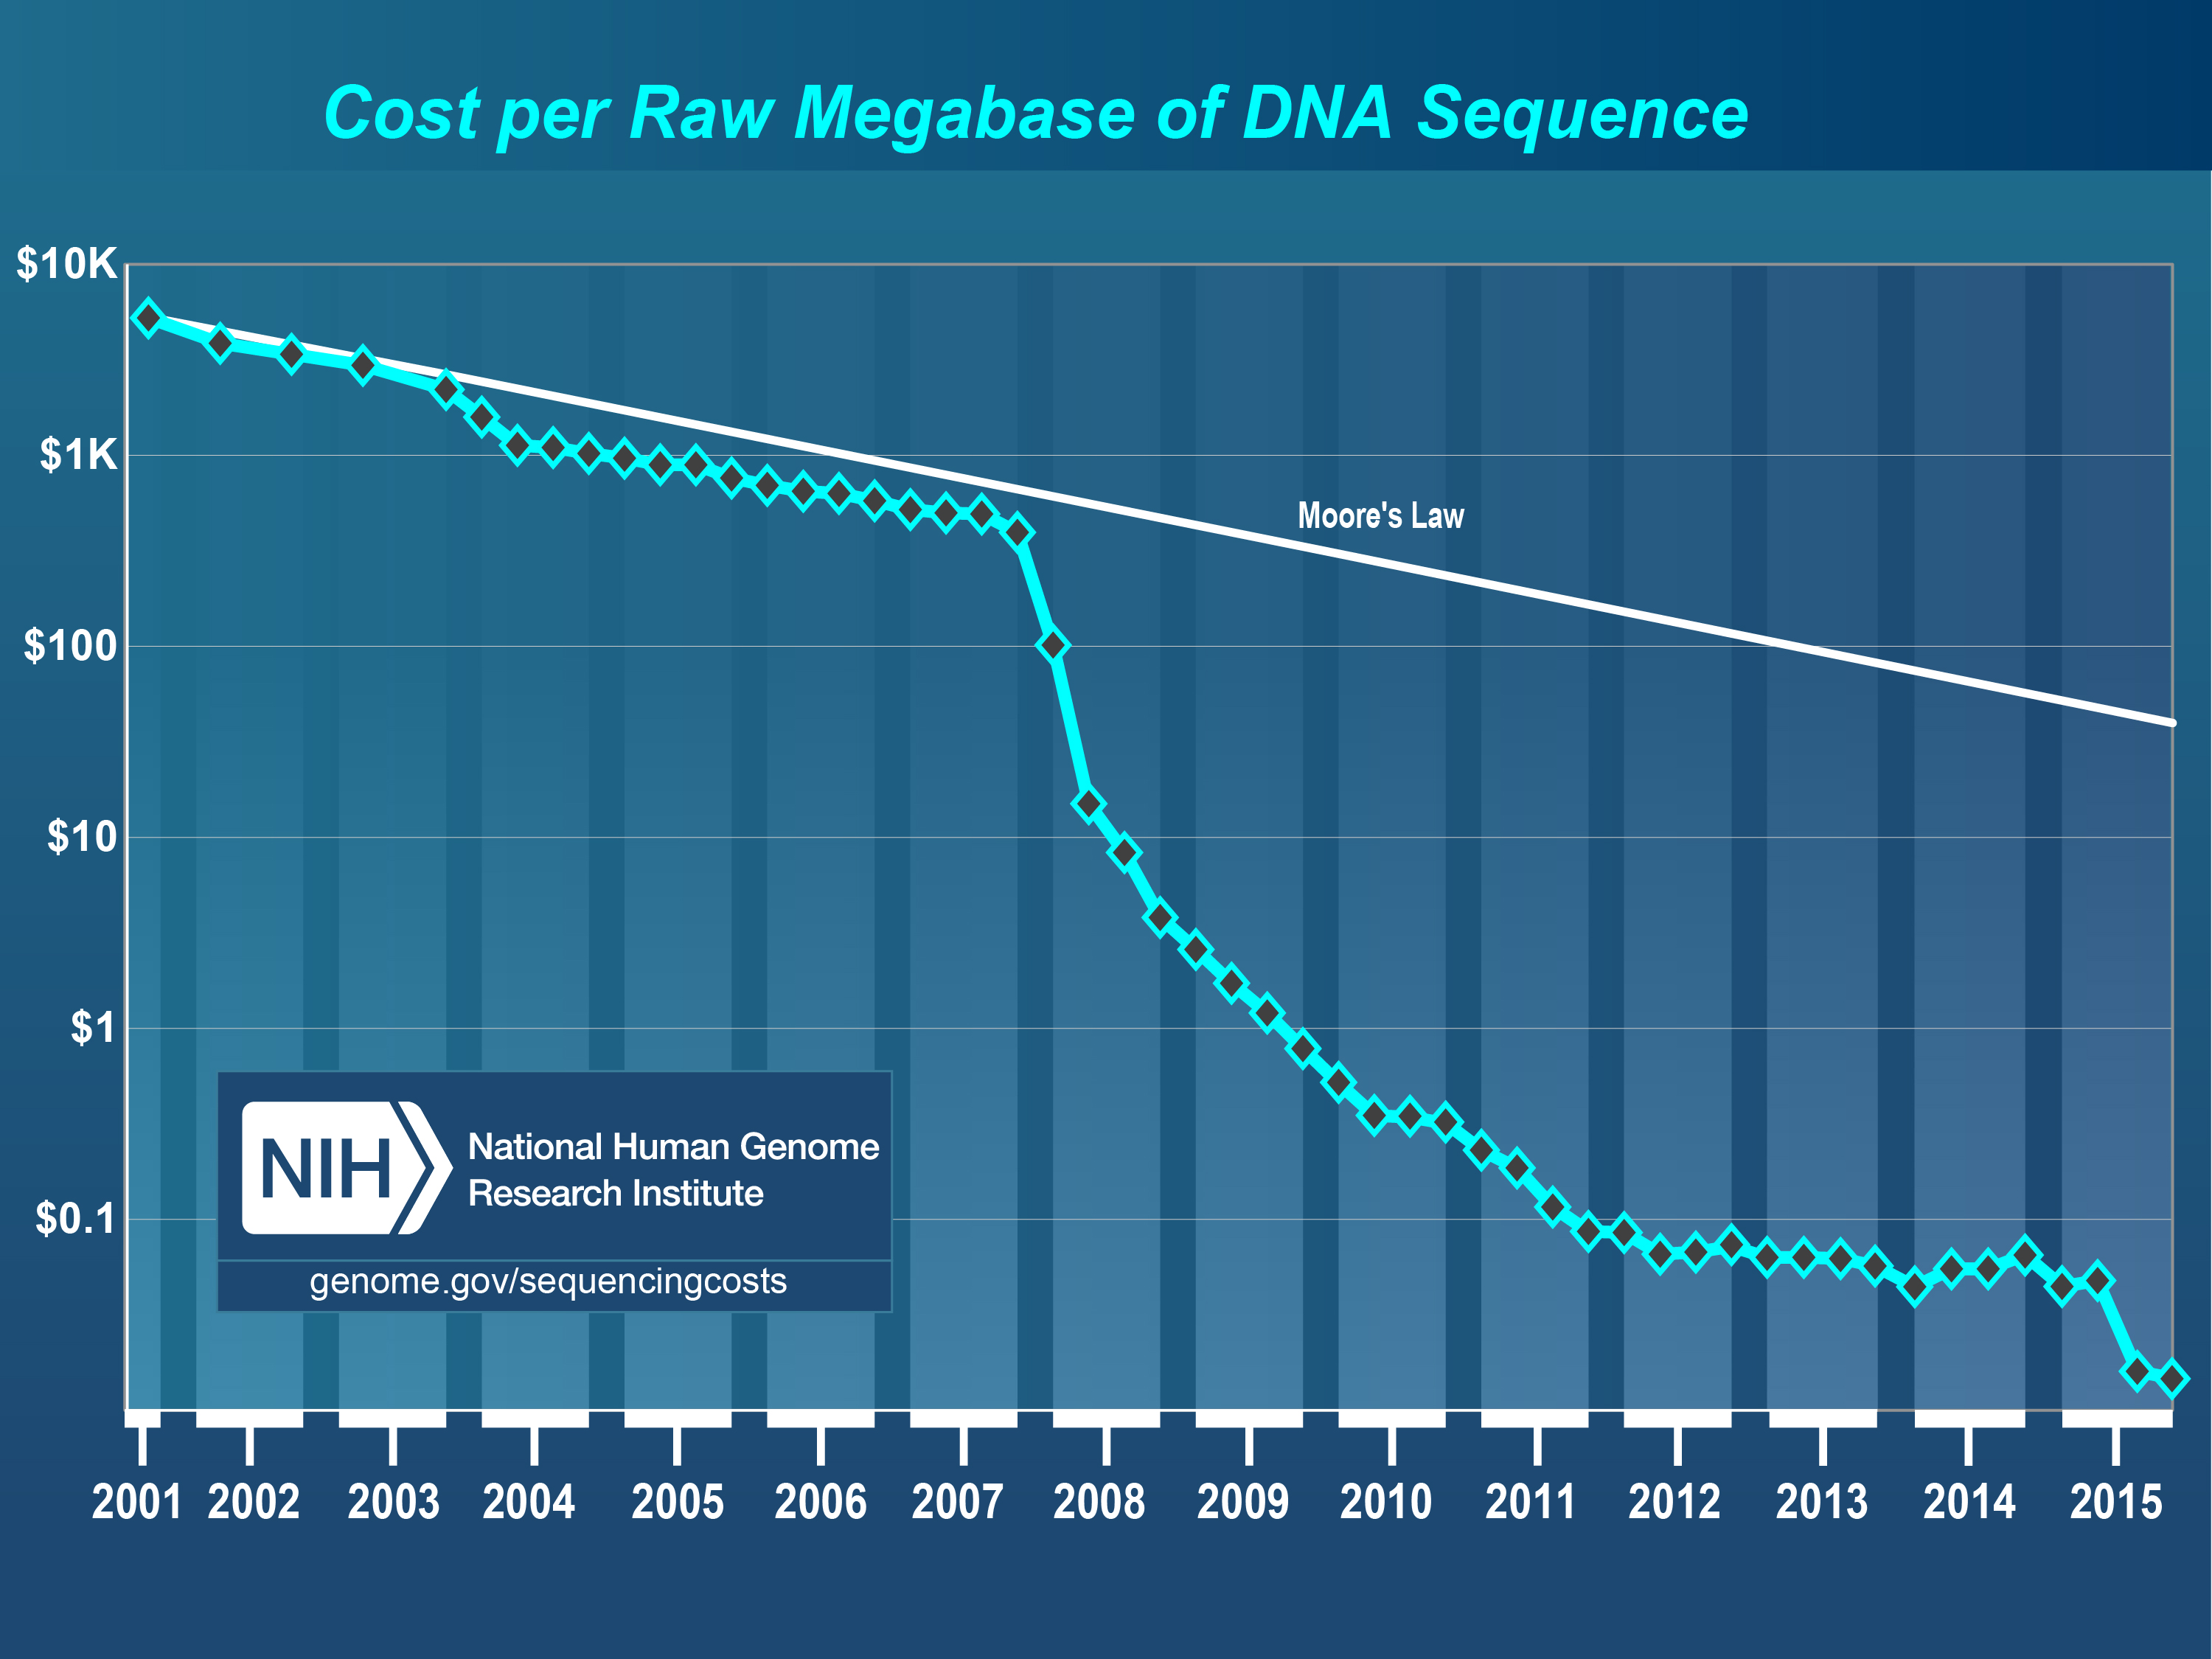
\includegraphics[width=1.0\textwidth]{costperMb2015_4.jpg}}
\end{center}
\caption[Cost per raw megabase of DNA sequence from 2001 to 2015]{Cost per raw megabase of DNA sequence from 2001 to 2015. Straight line - Moore's Law, blue curve - cost in US dollars, Y-axis scale is logarithmic. Graph reproduced from \citep{wetterstrand2016}}
\end{figure}

\chapter{}
\vspace*{-0.3in}
\begin{figure}[hb!]
\begin{center}
\makebox[\textwidth][c]{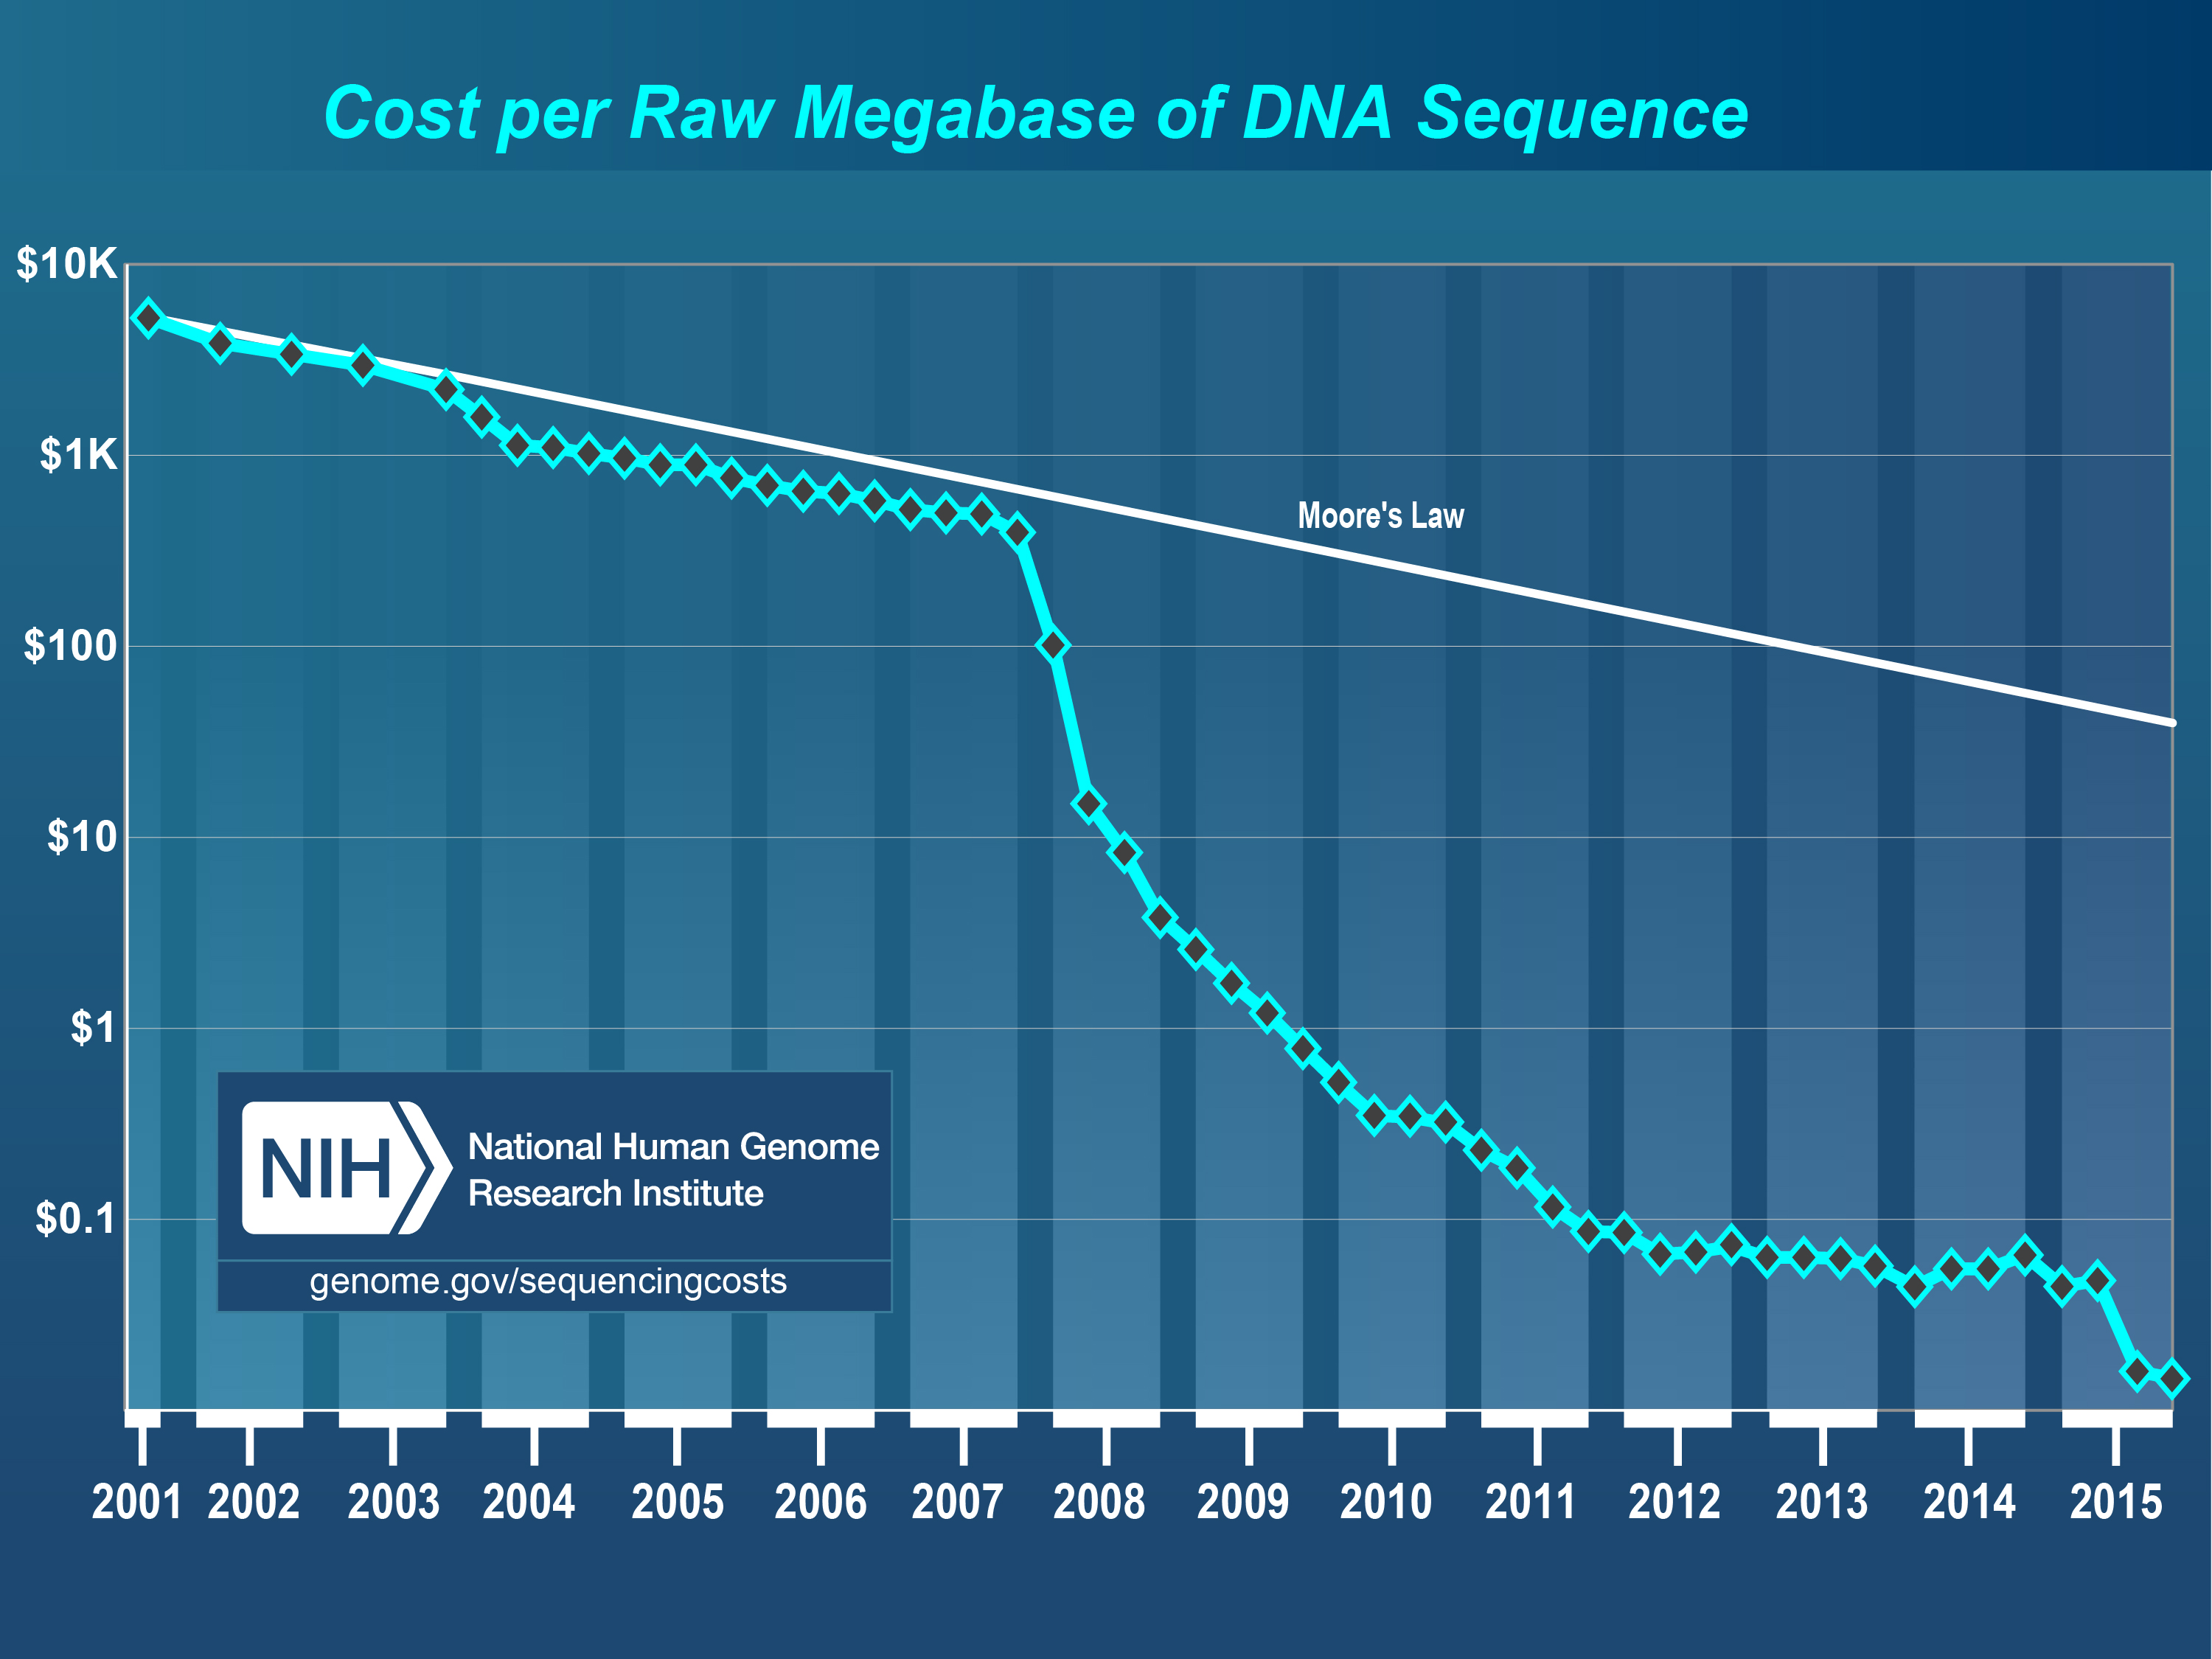
\includegraphics[width=1.0\textwidth]{costperMb2015_4.jpg}}
\end{center}
\caption[Cost per raw megabase of DNA sequence from 2001 to 2015]{Cost per raw megabase of DNA sequence from 2001 to 2015. Straight line - Moore's Law, blue curve - cost in US dollars, Y-axis scale is logarithmic. Graph reproduced from \citep{wetterstrand2016}}
\end{figure}

\chapter{}
\begin{figure}[hb!]
\begin{center}
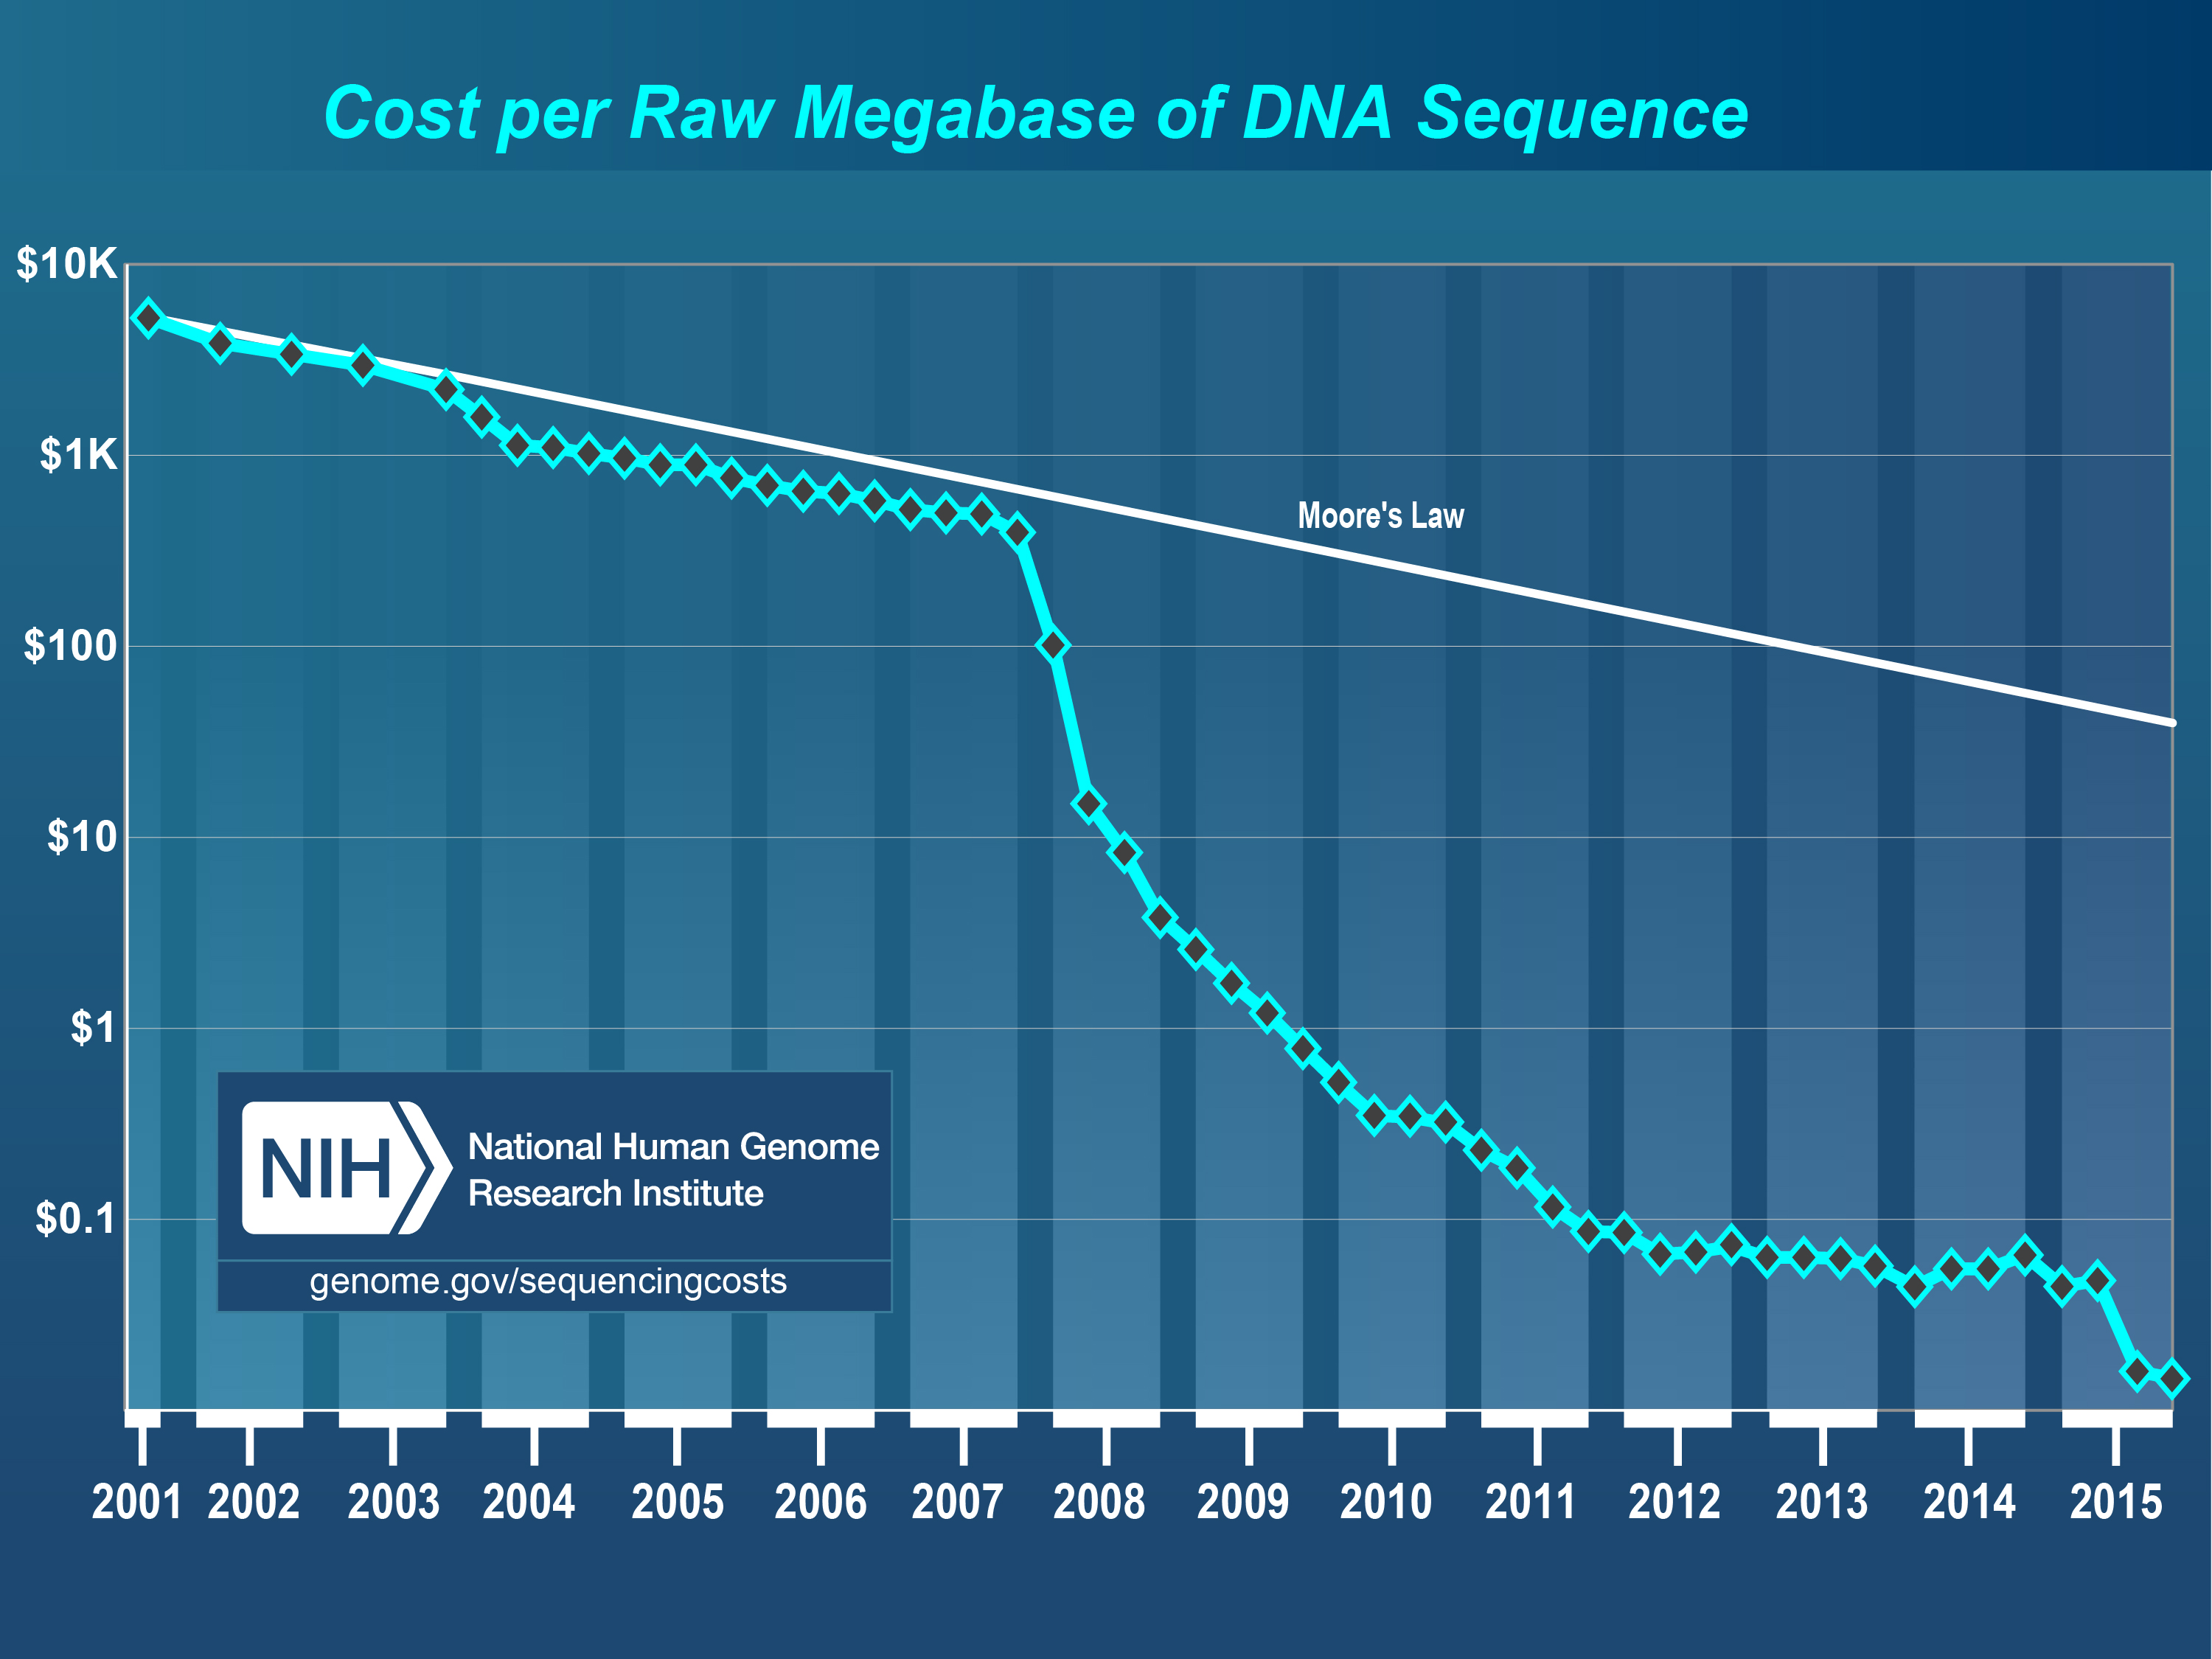
\includegraphics[scale=0.5]{costperMb2015_4.jpg}
\end{center}
\caption[Cost per raw megabase of DNA sequence from 2001 to 2015]{Cost per raw megabase of DNA sequence from 2001 to 2015. Straight line - Moore's Law, blue curve - cost in US dollars, Y-axis scale is logarithmic. Graph reproduced from \citep{wetterstrand2016}}
\end{figure}

\chapter{}
\begin{figure}[hb!]
\begin{center}
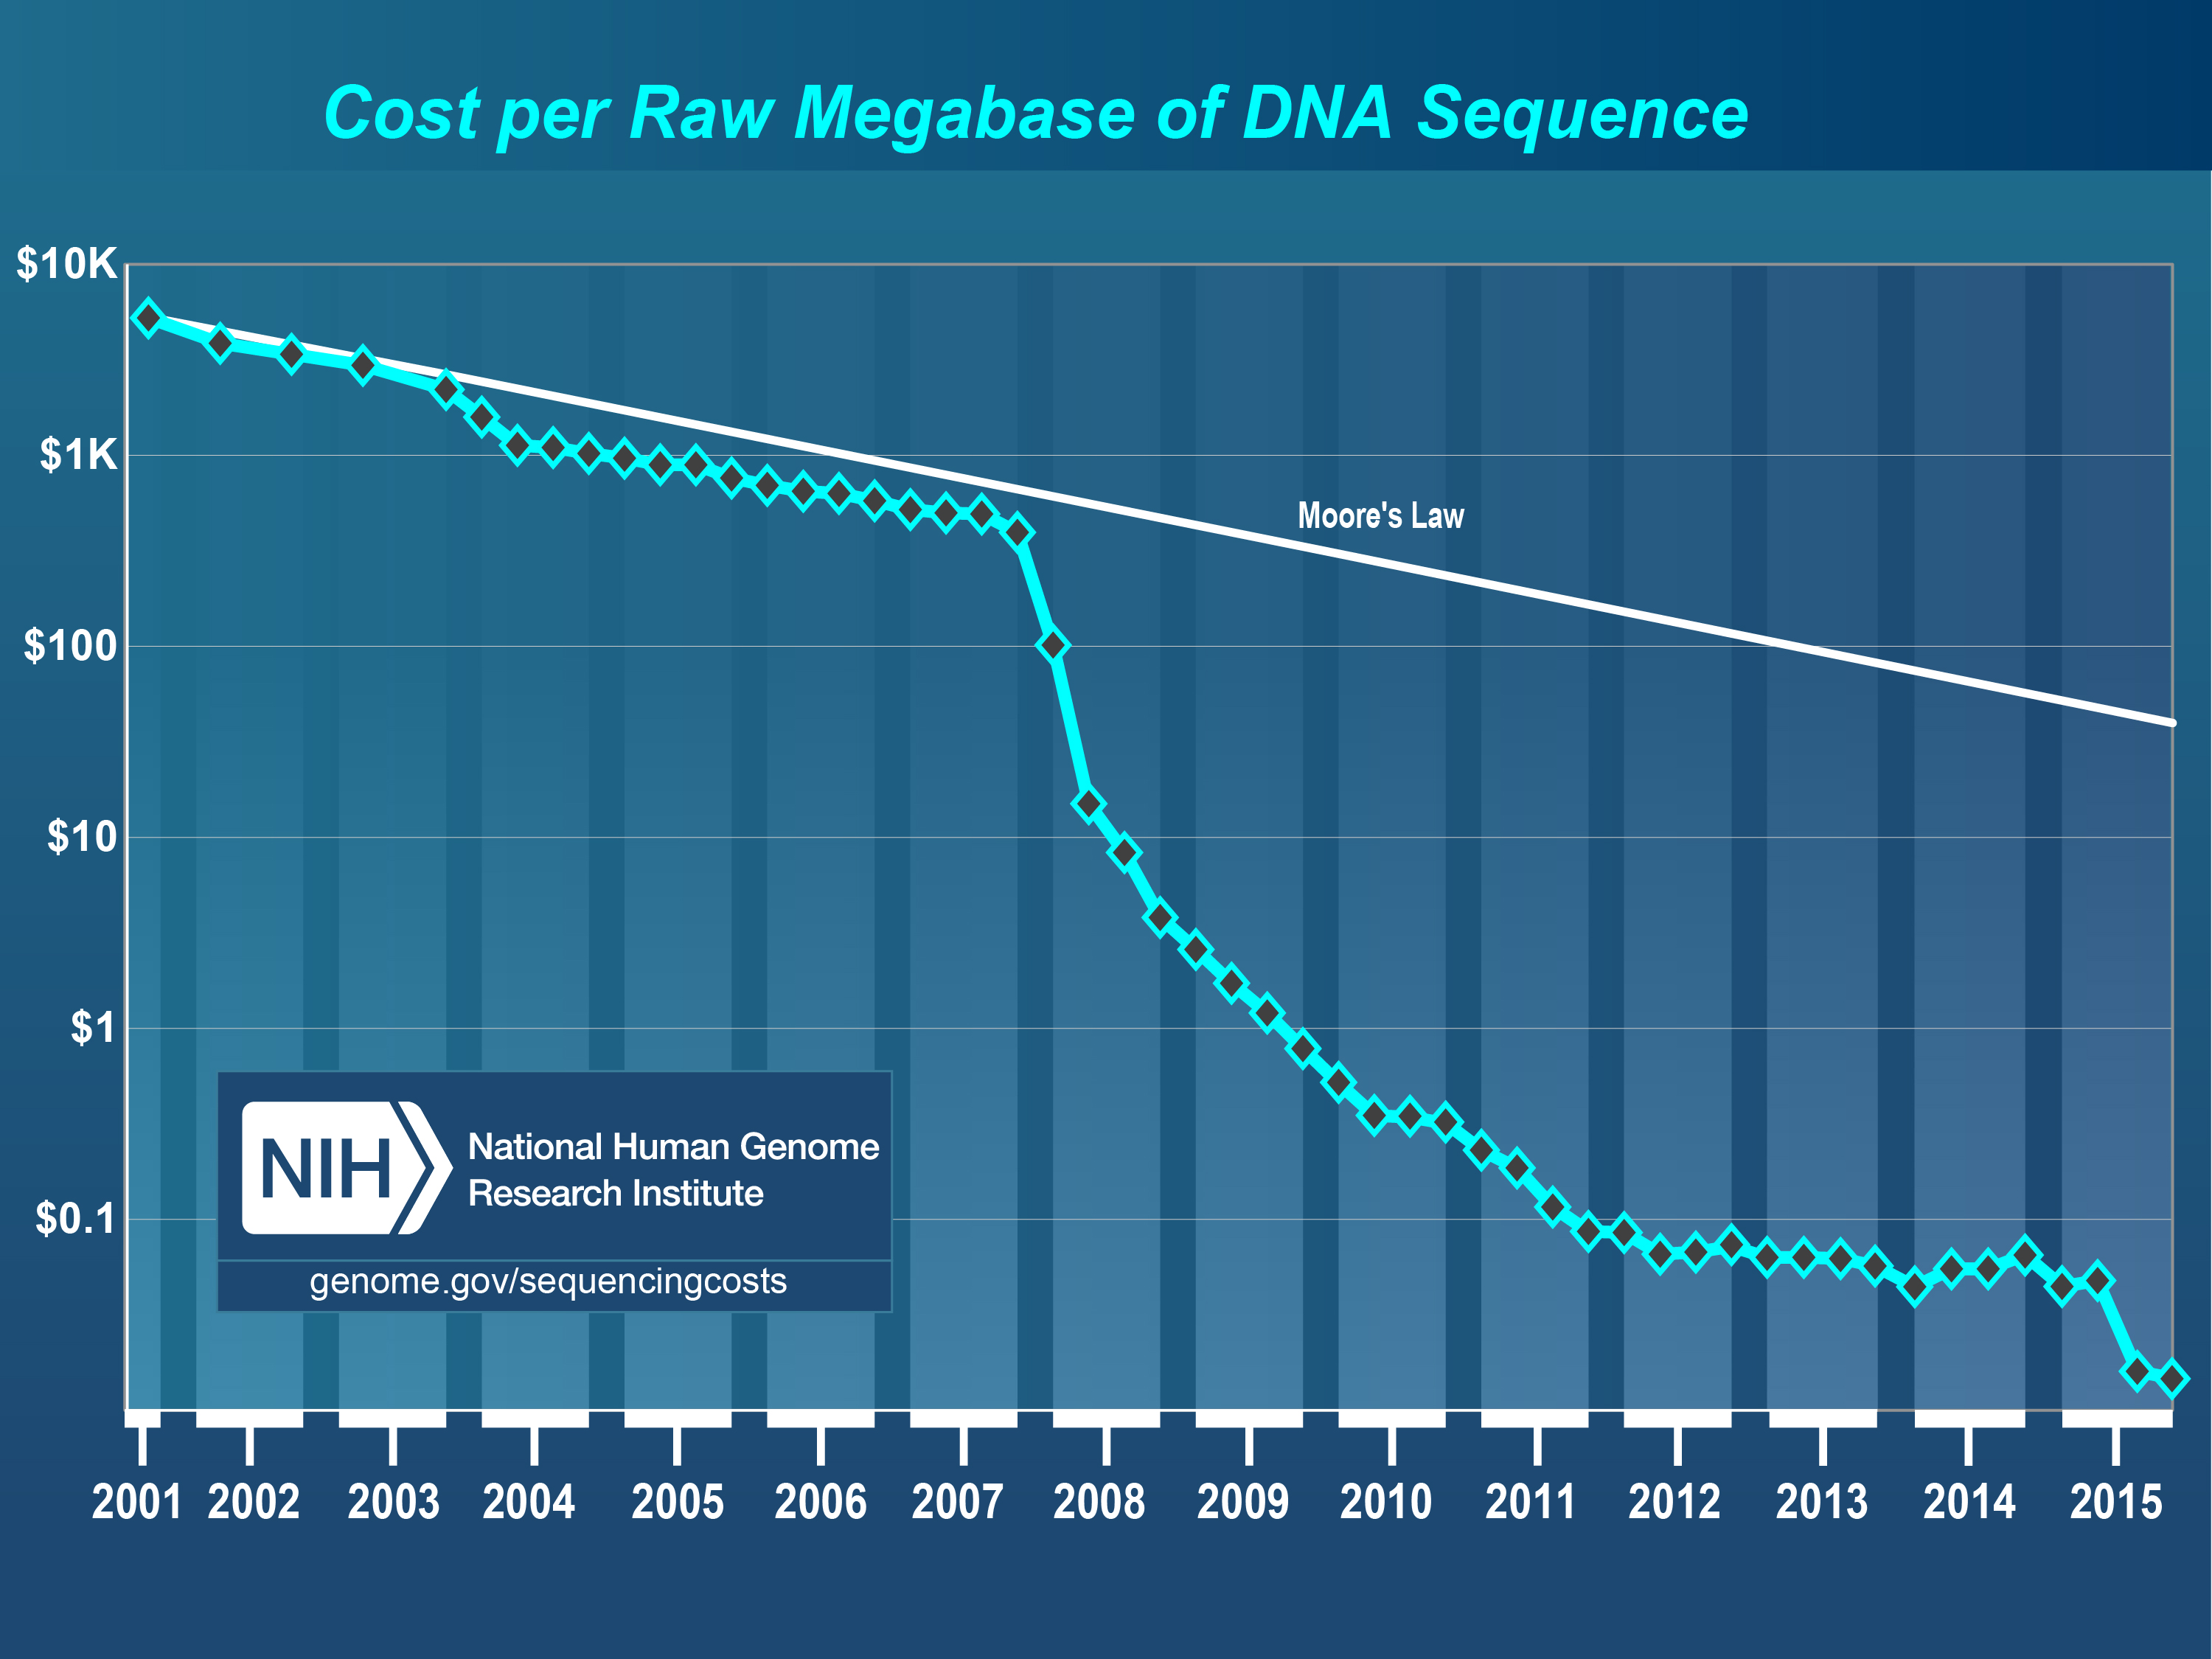
\includegraphics[scale=0.5]{costperMb2015_4.jpg}
\end{center}
\caption[Cost per raw megabase of DNA sequence from 2001 to 2015]{Cost per raw megabase of DNA sequence from 2001 to 2015. Straight line - Moore's Law, blue curve - cost in US dollars, Y-axis scale is logarithmic. Graph reproduced from \citep{wetterstrand2016}}
\end{figure}

\chapter{}
\begin{figure}[hb!]
\begin{center}
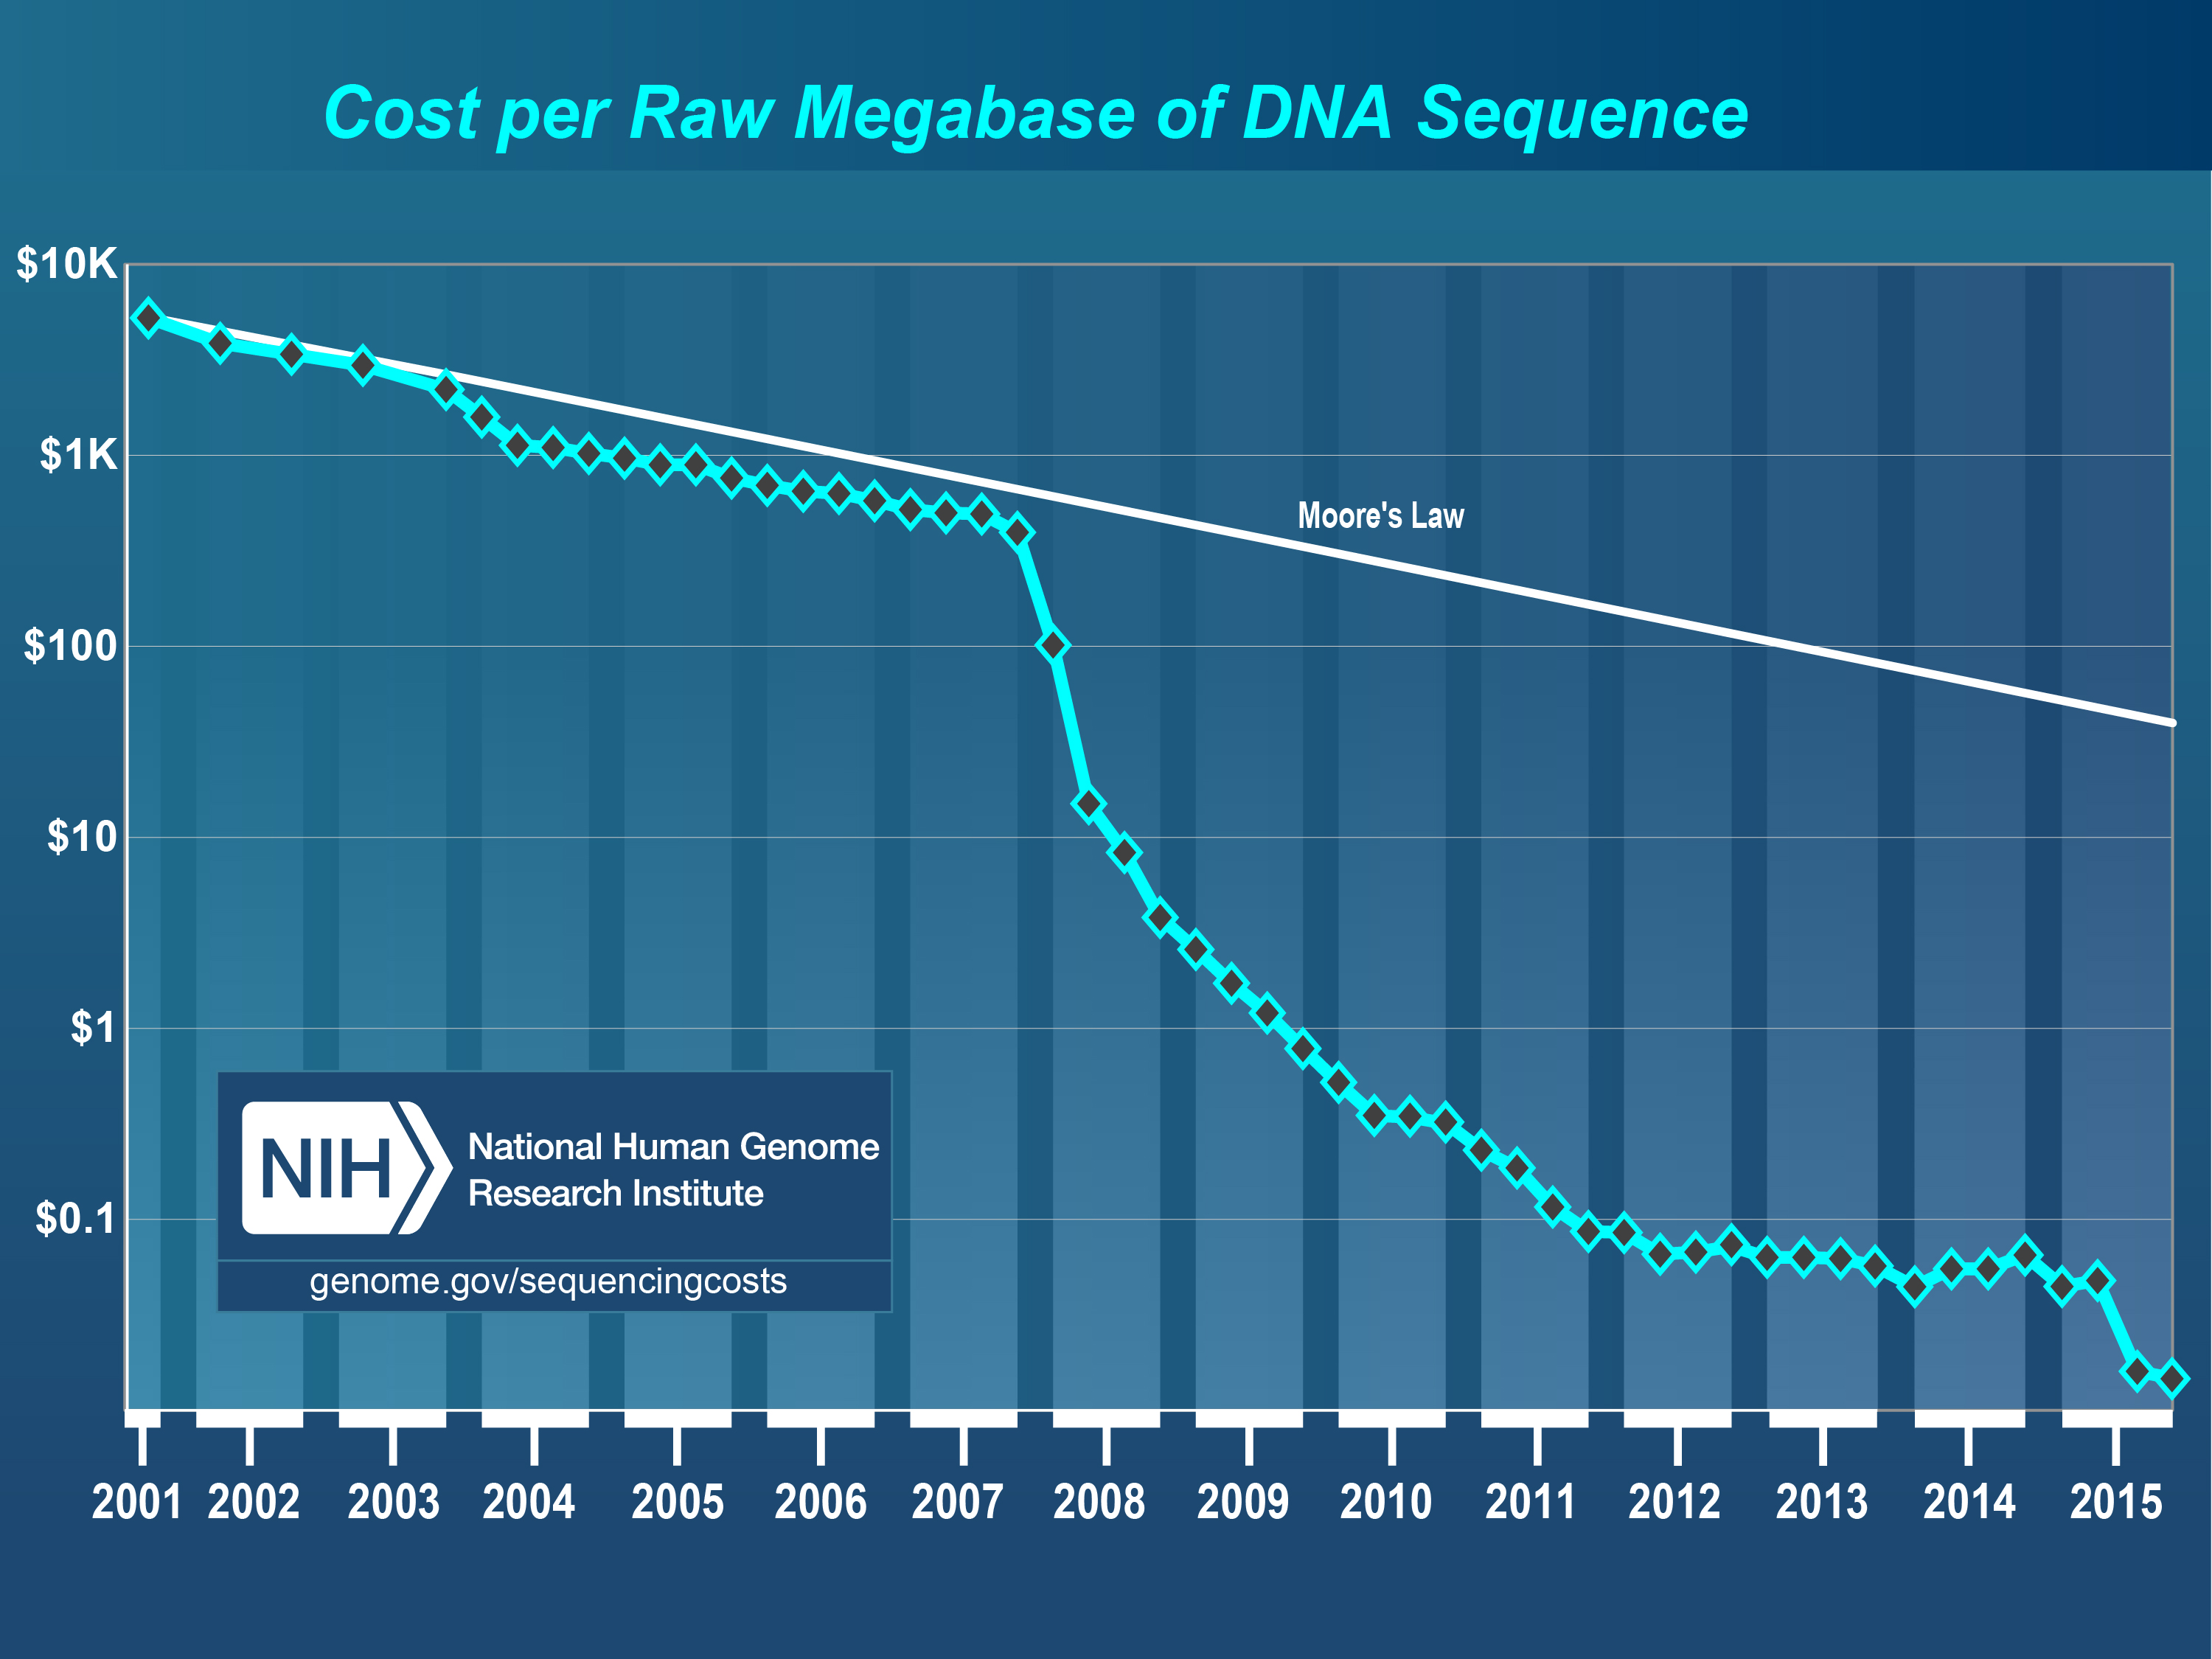
\includegraphics[scale=0.5]{costperMb2015_4.jpg}
\end{center}
\caption[Cost per raw megabase of DNA sequence from 2001 to 2015]{Cost per raw megabase of DNA sequence from 2001 to 2015. Straight line - Moore's Law, blue curve - cost in US dollars, Y-axis scale is logarithmic. Graph reproduced from \citep{wetterstrand2016}}
\end{figure}



\end{document}
